\documentclass[twoside]{book}

% Packages required by doxygen
\usepackage{fixltx2e}
\usepackage{calc}
\usepackage{doxygen}
\usepackage[export]{adjustbox} % also loads graphicx
\usepackage{graphicx}
\usepackage[utf8]{inputenc}
\usepackage{makeidx}
\usepackage{multicol}
\usepackage{multirow}
\PassOptionsToPackage{warn}{textcomp}
\usepackage{textcomp}
\usepackage[nointegrals]{wasysym}
\usepackage[table]{xcolor}

% Font selection
\usepackage[T1]{fontenc}
\usepackage[scaled=.90]{helvet}
\usepackage{courier}
\usepackage{amssymb}
\usepackage{sectsty}
\renewcommand{\familydefault}{\sfdefault}
\allsectionsfont{%
  \fontseries{bc}\selectfont%
  \color{darkgray}%
}
\renewcommand{\DoxyLabelFont}{%
  \fontseries{bc}\selectfont%
  \color{darkgray}%
}
\newcommand{\+}{\discretionary{\mbox{\scriptsize$\hookleftarrow$}}{}{}}

% Page & text layout
\usepackage{geometry}
\geometry{%
  a4paper,%
  top=2.5cm,%
  bottom=2.5cm,%
  left=2.5cm,%
  right=2.5cm%
}
\tolerance=750
\hfuzz=15pt
\hbadness=750
\setlength{\emergencystretch}{15pt}
\setlength{\parindent}{0cm}
\setlength{\parskip}{3ex plus 2ex minus 2ex}
\makeatletter
\renewcommand{\paragraph}{%
  \@startsection{paragraph}{4}{0ex}{-1.0ex}{1.0ex}{%
    \normalfont\normalsize\bfseries\SS@parafont%
  }%
}
\renewcommand{\subparagraph}{%
  \@startsection{subparagraph}{5}{0ex}{-1.0ex}{1.0ex}{%
    \normalfont\normalsize\bfseries\SS@subparafont%
  }%
}
\makeatother

% Headers & footers
\usepackage{fancyhdr}
\pagestyle{fancyplain}
\fancyhead[LE]{\fancyplain{}{\bfseries\thepage}}
\fancyhead[CE]{\fancyplain{}{}}
\fancyhead[RE]{\fancyplain{}{\bfseries\leftmark}}
\fancyhead[LO]{\fancyplain{}{\bfseries\rightmark}}
\fancyhead[CO]{\fancyplain{}{}}
\fancyhead[RO]{\fancyplain{}{\bfseries\thepage}}
\fancyfoot[LE]{\fancyplain{}{}}
\fancyfoot[CE]{\fancyplain{}{}}
\fancyfoot[RE]{\fancyplain{}{\bfseries\scriptsize Generated by Doxygen }}
\fancyfoot[LO]{\fancyplain{}{\bfseries\scriptsize Generated by Doxygen }}
\fancyfoot[CO]{\fancyplain{}{}}
\fancyfoot[RO]{\fancyplain{}{}}
\renewcommand{\footrulewidth}{0.4pt}
\renewcommand{\chaptermark}[1]{%
  \markboth{#1}{}%
}
\renewcommand{\sectionmark}[1]{%
  \markright{\thesection\ #1}%
}

% Indices & bibliography
\usepackage{natbib}
\usepackage[titles]{tocloft}
\setcounter{tocdepth}{3}
\setcounter{secnumdepth}{5}
\makeindex

% Hyperlinks (required, but should be loaded last)
\usepackage{ifpdf}
\ifpdf
  \usepackage[pdftex,pagebackref=true]{hyperref}
\else
  \usepackage[ps2pdf,pagebackref=true]{hyperref}
\fi
\hypersetup{%
  colorlinks=true,%
  linkcolor=blue,%
  citecolor=blue,%
  unicode%
}

% Custom commands
\newcommand{\clearemptydoublepage}{%
  \newpage{\pagestyle{empty}\cleardoublepage}%
}

\usepackage{caption}
\captionsetup{labelsep=space,justification=centering,font={bf},singlelinecheck=off,skip=4pt,position=top}

%===== C O N T E N T S =====

\begin{document}

% Titlepage & ToC
\hypersetup{pageanchor=false,
             bookmarksnumbered=true,
             pdfencoding=unicode
            }
\pagenumbering{alph}
\begin{titlepage}
\vspace*{7cm}
\begin{center}%
{\Large My Project }\\
\vspace*{1cm}
{\large Generated by Doxygen 1.8.14}\\
\end{center}
\end{titlepage}
\clearemptydoublepage
\pagenumbering{roman}
\tableofcontents
\clearemptydoublepage
\pagenumbering{arabic}
\hypersetup{pageanchor=true}

%--- Begin generated contents ---
\chapter{R\+E\+A\+D\+ME}
\label{md_out_production_fa18-cs242-assignment1__r_e_a_d_m_e}
\Hypertarget{md_out_production_fa18-cs242-assignment1__r_e_a_d_m_e}
\input{md_out_production_fa18-cs242-assignment1__r_e_a_d_m_e}
\chapter{R\+E\+A\+D\+ME}
\label{md__r_e_a_d_m_e}
\Hypertarget{md__r_e_a_d_m_e}
\input{md__r_e_a_d_m_e}
\chapter{Hierarchical Index}
\section{Class Hierarchy}
This inheritance list is sorted roughly, but not completely, alphabetically\+:\begin{DoxyCompactList}
\item \contentsline{section}{tests.\+Bishop\+Tests}{\pageref{classtests_1_1_bishop_tests}}{}
\item \contentsline{section}{main.\+Board}{\pageref{classmain_1_1_board}}{}
\item \contentsline{section}{tests.\+Checkmate\+Tests}{\pageref{classtests_1_1_checkmate_tests}}{}
\item \contentsline{section}{tests.\+Crab\+Tests}{\pageref{classtests_1_1_crab_tests}}{}
\item \contentsline{section}{G\+U\+I.\+G\+U\+I\+Board}{\pageref{class_g_u_i_1_1_g_u_i_board}}{}
\item J\+Frame\begin{DoxyCompactList}
\item \contentsline{section}{controller.\+Controller}{\pageref{classcontroller_1_1_controller}}{}
\end{DoxyCompactList}
\item J\+Panel\begin{DoxyCompactList}
\item \contentsline{section}{G\+U\+I.\+G\+U\+I\+Board.\+Table}{\pageref{class_g_u_i_1_1_g_u_i_board_1_1_table}}{}
\item \contentsline{section}{G\+U\+I.\+G\+U\+I\+Menu}{\pageref{class_g_u_i_1_1_g_u_i_menu}}{}
\end{DoxyCompactList}
\item \contentsline{section}{tests.\+King\+Tests}{\pageref{classtests_1_1_king_tests}}{}
\item \contentsline{section}{tests.\+Knight\+Tests}{\pageref{classtests_1_1_knight_tests}}{}
\item \contentsline{section}{G\+U\+I.\+Main}{\pageref{class_g_u_i_1_1_main}}{}
\item \contentsline{section}{tests.\+Ox\+Tests}{\pageref{classtests_1_1_ox_tests}}{}
\item \contentsline{section}{tests.\+Pawn\+Tests}{\pageref{classtests_1_1_pawn_tests}}{}
\item \contentsline{section}{main.\+Pieces}{\pageref{classmain_1_1_pieces}}{}
\begin{DoxyCompactList}
\item \contentsline{section}{main.\+Bishop}{\pageref{classmain_1_1_bishop}}{}
\item \contentsline{section}{main.\+Crab}{\pageref{classmain_1_1_crab}}{}
\item \contentsline{section}{main.\+King}{\pageref{classmain_1_1_king}}{}
\item \contentsline{section}{main.\+Knight}{\pageref{classmain_1_1_knight}}{}
\item \contentsline{section}{main.\+Ox}{\pageref{classmain_1_1_ox}}{}
\item \contentsline{section}{main.\+Pawn}{\pageref{classmain_1_1_pawn}}{}
\item \contentsline{section}{main.\+Queen}{\pageref{classmain_1_1_queen}}{}
\item \contentsline{section}{main.\+Rook}{\pageref{classmain_1_1_rook}}{}
\end{DoxyCompactList}
\item \contentsline{section}{tests.\+Queen\+Tests}{\pageref{classtests_1_1_queen_tests}}{}
\item \contentsline{section}{tests.\+Rook\+Tests}{\pageref{classtests_1_1_rook_tests}}{}
\item \contentsline{section}{tests.\+Stalemate\+Tests}{\pageref{classtests_1_1_stalemate_tests}}{}
\item \contentsline{section}{tests.\+Undo\+Tests}{\pageref{classtests_1_1_undo_tests}}{}
\end{DoxyCompactList}

\chapter{Class Index}
\section{Class List}
Here are the classes, structs, unions and interfaces with brief descriptions\+:\begin{DoxyCompactList}
\item\contentsline{section}{\mbox{\hyperlink{classmain_1_1_bishop}{main.\+Bishop}} }{\pageref{classmain_1_1_bishop}}{}
\item\contentsline{section}{\mbox{\hyperlink{classtests_1_1_bishop_tests}{tests.\+Bishop\+Tests}} }{\pageref{classtests_1_1_bishop_tests}}{}
\item\contentsline{section}{\mbox{\hyperlink{classmain_1_1_board}{main.\+Board}} }{\pageref{classmain_1_1_board}}{}
\item\contentsline{section}{\mbox{\hyperlink{classtests_1_1_checkmate_tests}{tests.\+Checkmate\+Tests}} }{\pageref{classtests_1_1_checkmate_tests}}{}
\item\contentsline{section}{\mbox{\hyperlink{classcontroller_1_1_controller}{controller.\+Controller}} }{\pageref{classcontroller_1_1_controller}}{}
\item\contentsline{section}{\mbox{\hyperlink{classmain_1_1_crab}{main.\+Crab}} }{\pageref{classmain_1_1_crab}}{}
\item\contentsline{section}{\mbox{\hyperlink{classtests_1_1_crab_tests}{tests.\+Crab\+Tests}} }{\pageref{classtests_1_1_crab_tests}}{}
\item\contentsline{section}{\mbox{\hyperlink{class_g_u_i_1_1_g_u_i_board}{G\+U\+I.\+G\+U\+I\+Board}} }{\pageref{class_g_u_i_1_1_g_u_i_board}}{}
\item\contentsline{section}{\mbox{\hyperlink{class_g_u_i_1_1_g_u_i_menu}{G\+U\+I.\+G\+U\+I\+Menu}} }{\pageref{class_g_u_i_1_1_g_u_i_menu}}{}
\item\contentsline{section}{\mbox{\hyperlink{classmain_1_1_king}{main.\+King}} }{\pageref{classmain_1_1_king}}{}
\item\contentsline{section}{\mbox{\hyperlink{classtests_1_1_king_tests}{tests.\+King\+Tests}} }{\pageref{classtests_1_1_king_tests}}{}
\item\contentsline{section}{\mbox{\hyperlink{classmain_1_1_knight}{main.\+Knight}} }{\pageref{classmain_1_1_knight}}{}
\item\contentsline{section}{\mbox{\hyperlink{classtests_1_1_knight_tests}{tests.\+Knight\+Tests}} }{\pageref{classtests_1_1_knight_tests}}{}
\item\contentsline{section}{\mbox{\hyperlink{class_g_u_i_1_1_main}{G\+U\+I.\+Main}} }{\pageref{class_g_u_i_1_1_main}}{}
\item\contentsline{section}{\mbox{\hyperlink{classmain_1_1_ox}{main.\+Ox}} }{\pageref{classmain_1_1_ox}}{}
\item\contentsline{section}{\mbox{\hyperlink{classtests_1_1_ox_tests}{tests.\+Ox\+Tests}} }{\pageref{classtests_1_1_ox_tests}}{}
\item\contentsline{section}{\mbox{\hyperlink{classmain_1_1_pawn}{main.\+Pawn}} }{\pageref{classmain_1_1_pawn}}{}
\item\contentsline{section}{\mbox{\hyperlink{classtests_1_1_pawn_tests}{tests.\+Pawn\+Tests}} }{\pageref{classtests_1_1_pawn_tests}}{}
\item\contentsline{section}{\mbox{\hyperlink{classmain_1_1_pieces}{main.\+Pieces}} }{\pageref{classmain_1_1_pieces}}{}
\item\contentsline{section}{\mbox{\hyperlink{classmain_1_1_queen}{main.\+Queen}} }{\pageref{classmain_1_1_queen}}{}
\item\contentsline{section}{\mbox{\hyperlink{classtests_1_1_queen_tests}{tests.\+Queen\+Tests}} }{\pageref{classtests_1_1_queen_tests}}{}
\item\contentsline{section}{\mbox{\hyperlink{classmain_1_1_rook}{main.\+Rook}} }{\pageref{classmain_1_1_rook}}{}
\item\contentsline{section}{\mbox{\hyperlink{classtests_1_1_rook_tests}{tests.\+Rook\+Tests}} }{\pageref{classtests_1_1_rook_tests}}{}
\item\contentsline{section}{\mbox{\hyperlink{classtests_1_1_stalemate_tests}{tests.\+Stalemate\+Tests}} }{\pageref{classtests_1_1_stalemate_tests}}{}
\item\contentsline{section}{\mbox{\hyperlink{class_g_u_i_1_1_g_u_i_board_1_1_table}{G\+U\+I.\+G\+U\+I\+Board.\+Table}} }{\pageref{class_g_u_i_1_1_g_u_i_board_1_1_table}}{}
\item\contentsline{section}{\mbox{\hyperlink{classtests_1_1_undo_tests}{tests.\+Undo\+Tests}} }{\pageref{classtests_1_1_undo_tests}}{}
\end{DoxyCompactList}

\chapter{Class Documentation}
\hypertarget{classmain_1_1_bishop}{}\section{main.\+Bishop Class Reference}
\label{classmain_1_1_bishop}\index{main.\+Bishop@{main.\+Bishop}}
Inheritance diagram for main.\+Bishop\+:\begin{figure}[H]
\begin{center}
\leavevmode
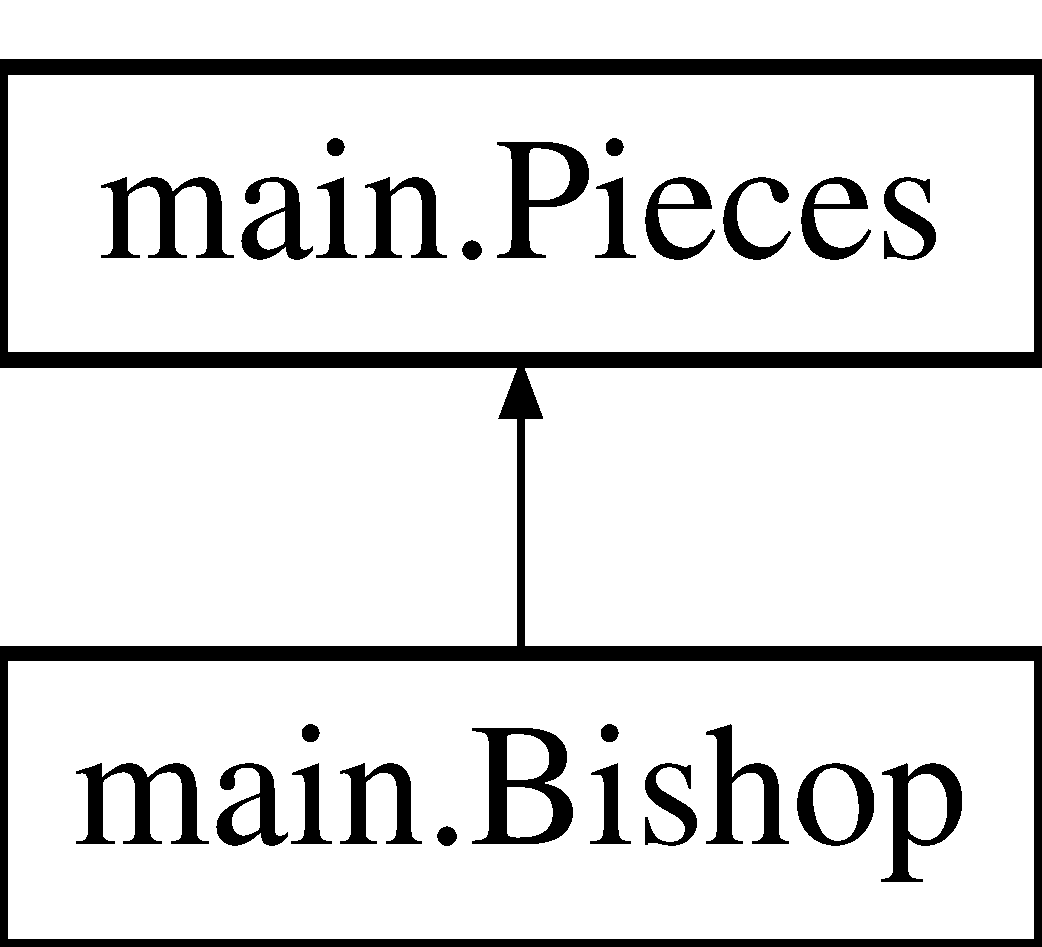
\includegraphics[height=2.000000cm]{classmain_1_1_bishop}
\end{center}
\end{figure}
\subsection*{Public Member Functions}
\begin{DoxyCompactItemize}
\item 
\mbox{\hyperlink{classmain_1_1_bishop_a7bd138f6235b21e03abd144019550dca}{Bishop}} (int x, int y, int player)
\item 
\mbox{\Hypertarget{classmain_1_1_bishop_a94831e04973f57ce029300fa886c3f9d}\label{classmain_1_1_bishop_a94831e04973f57ce029300fa886c3f9d}} 
boolean {\bfseries is\+Valid\+Move} (int newX, int newY)
\item 
boolean \mbox{\hyperlink{classmain_1_1_bishop_a8690770e84015412d261577a0a30dadd}{valid\+Move}} (int newX, int newY, \mbox{\hyperlink{classmain_1_1_board}{Board}} board)
\item 
boolean \mbox{\hyperlink{classmain_1_1_bishop_a669732f2463b39beba91497d5345d48b}{could\+Be\+Stopped}} (int newX, int newY, \mbox{\hyperlink{classmain_1_1_board}{Board}} board)
\item 
boolean \mbox{\hyperlink{classmain_1_1_bishop_a8fa8870068eaa19b494949ac7b62f7c7}{is\+Movable}} (\mbox{\hyperlink{classmain_1_1_board}{Board}} board)
\end{DoxyCompactItemize}
\subsection*{Additional Inherited Members}


\subsection{Detailed Description}
\begin{DoxyAuthor}{Author}
kaichenle 
\end{DoxyAuthor}


\subsection{Constructor \& Destructor Documentation}
\mbox{\Hypertarget{classmain_1_1_bishop_a7bd138f6235b21e03abd144019550dca}\label{classmain_1_1_bishop_a7bd138f6235b21e03abd144019550dca}} 
\index{main\+::\+Bishop@{main\+::\+Bishop}!Bishop@{Bishop}}
\index{Bishop@{Bishop}!main\+::\+Bishop@{main\+::\+Bishop}}
\subsubsection{\texorpdfstring{Bishop()}{Bishop()}}
{\footnotesize\ttfamily main.\+Bishop.\+Bishop (\begin{DoxyParamCaption}\item[{int}]{x,  }\item[{int}]{y,  }\item[{int}]{player }\end{DoxyParamCaption})\hspace{0.3cm}{\ttfamily [inline]}}

constructor 
\begin{DoxyParams}{Parameters}
{\em x} & x\+Coord \\
\hline
{\em y} & y\+Coord \\
\hline
{\em player} & player 1 or 2 \\
\hline
\end{DoxyParams}


\subsection{Member Function Documentation}
\mbox{\Hypertarget{classmain_1_1_bishop_a669732f2463b39beba91497d5345d48b}\label{classmain_1_1_bishop_a669732f2463b39beba91497d5345d48b}} 
\index{main\+::\+Bishop@{main\+::\+Bishop}!could\+Be\+Stopped@{could\+Be\+Stopped}}
\index{could\+Be\+Stopped@{could\+Be\+Stopped}!main\+::\+Bishop@{main\+::\+Bishop}}
\subsubsection{\texorpdfstring{could\+Be\+Stopped()}{couldBeStopped()}}
{\footnotesize\ttfamily boolean main.\+Bishop.\+could\+Be\+Stopped (\begin{DoxyParamCaption}\item[{int}]{newX,  }\item[{int}]{newY,  }\item[{\mbox{\hyperlink{classmain_1_1_board}{Board}}}]{board }\end{DoxyParamCaption})\hspace{0.3cm}{\ttfamily [inline]}}

if any pieces could stop input bishop or queen(diaganol) piece from x,y to newX newY 
\begin{DoxyParams}{Parameters}
{\em newX} & end x\+Coord \\
\hline
{\em newY} & end y\+Coord \\
\hline
{\em board} & the game will play on \\
\hline
\end{DoxyParams}
\begin{DoxyReturn}{Returns}
true if there is a piece exists otherwise false 
\end{DoxyReturn}
\mbox{\Hypertarget{classmain_1_1_bishop_a8fa8870068eaa19b494949ac7b62f7c7}\label{classmain_1_1_bishop_a8fa8870068eaa19b494949ac7b62f7c7}} 
\index{main\+::\+Bishop@{main\+::\+Bishop}!is\+Movable@{is\+Movable}}
\index{is\+Movable@{is\+Movable}!main\+::\+Bishop@{main\+::\+Bishop}}
\subsubsection{\texorpdfstring{is\+Movable()}{isMovable()}}
{\footnotesize\ttfamily boolean main.\+Bishop.\+is\+Movable (\begin{DoxyParamCaption}\item[{\mbox{\hyperlink{classmain_1_1_board}{Board}}}]{board }\end{DoxyParamCaption})\hspace{0.3cm}{\ttfamily [inline]}}

helper functions check movability of bishop or queen(diaganol) 
\begin{DoxyParams}{Parameters}
{\em board} & the game will be on \\
\hline
\end{DoxyParams}
\begin{DoxyReturn}{Returns}
true if the input can move otherwise false 
\end{DoxyReturn}
\mbox{\Hypertarget{classmain_1_1_bishop_a8690770e84015412d261577a0a30dadd}\label{classmain_1_1_bishop_a8690770e84015412d261577a0a30dadd}} 
\index{main\+::\+Bishop@{main\+::\+Bishop}!valid\+Move@{valid\+Move}}
\index{valid\+Move@{valid\+Move}!main\+::\+Bishop@{main\+::\+Bishop}}
\subsubsection{\texorpdfstring{valid\+Move()}{validMove()}}
{\footnotesize\ttfamily boolean main.\+Bishop.\+valid\+Move (\begin{DoxyParamCaption}\item[{int}]{newX,  }\item[{int}]{newY,  }\item[{\mbox{\hyperlink{classmain_1_1_board}{Board}}}]{board }\end{DoxyParamCaption})\hspace{0.3cm}{\ttfamily [inline]}}

Helper functions check if it is a valid path to move \mbox{\hyperlink{classmain_1_1_bishop}{Bishop}}. It will be called inside move\+Chess with is\+Valid\+Move in each pieces subclass. This will check if there are pieces on the board that will influence the fact if it is valid to move chess 
\begin{DoxyParams}{Parameters}
{\em newX} & end y\+Coord \\
\hline
{\em newY} & end y\+Coord \\
\hline
{\em board} & the game will play on \\
\hline
\end{DoxyParams}
\begin{DoxyReturn}{Returns}
true if valid otherwise false 
\end{DoxyReturn}


The documentation for this class was generated from the following file\+:\begin{DoxyCompactItemize}
\item 
main/Bishop.\+java\end{DoxyCompactItemize}

\hypertarget{classtests_1_1_bishop_tests}{}\section{tests.\+Bishop\+Tests Class Reference}
\label{classtests_1_1_bishop_tests}\index{tests.\+Bishop\+Tests@{tests.\+Bishop\+Tests}}
\subsection*{Public Member Functions}
\begin{DoxyCompactItemize}
\item 
void \mbox{\hyperlink{classtests_1_1_bishop_tests_a8589665c879f8d73e7eda83873eb24e5}{should\+Move\+Bishop}} ()
\end{DoxyCompactItemize}


\subsection{Detailed Description}
\begin{DoxyAuthor}{Author}
kaichenle 
\end{DoxyAuthor}


\subsection{Member Function Documentation}
\mbox{\Hypertarget{classtests_1_1_bishop_tests_a8589665c879f8d73e7eda83873eb24e5}\label{classtests_1_1_bishop_tests_a8589665c879f8d73e7eda83873eb24e5}} 
\index{tests\+::\+Bishop\+Tests@{tests\+::\+Bishop\+Tests}!should\+Move\+Bishop@{should\+Move\+Bishop}}
\index{should\+Move\+Bishop@{should\+Move\+Bishop}!tests\+::\+Bishop\+Tests@{tests\+::\+Bishop\+Tests}}
\subsubsection{\texorpdfstring{should\+Move\+Bishop()}{shouldMoveBishop()}}
{\footnotesize\ttfamily void tests.\+Bishop\+Tests.\+should\+Move\+Bishop (\begin{DoxyParamCaption}{ }\end{DoxyParamCaption})\hspace{0.3cm}{\ttfamily [inline]}}

test the move\+Chess function 

The documentation for this class was generated from the following file\+:\begin{DoxyCompactItemize}
\item 
tests/Bishop\+Tests.\+java\end{DoxyCompactItemize}

\hypertarget{classmain_1_1_board}{}\section{main.\+Board Class Reference}
\label{classmain_1_1_board}\index{main.\+Board@{main.\+Board}}
\subsection*{Public Member Functions}
\begin{DoxyCompactItemize}
\item 
\mbox{\Hypertarget{classmain_1_1_board_aad7eb5429a65bcf5acb31b8032844833}\label{classmain_1_1_board_aad7eb5429a65bcf5acb31b8032844833}} 
boolean {\bfseries get\+Turns} ()
\item 
void \mbox{\hyperlink{classmain_1_1_board_a0b46a67725aeeab8d69ddb03735e14a0}{switch\+Turns}} ()
\item 
boolean \mbox{\hyperlink{classmain_1_1_board_ad4a1b505aa20498394a5905069e0dae6}{undo\+Valid}} ()
\item 
void \mbox{\hyperlink{classmain_1_1_board_a31c0049120e44edd6bf7d51ded24a513}{undo}} ()
\item 
\mbox{\hyperlink{classmain_1_1_board_a76177c2c47c5a55f8027c511d0e1e6d2}{Board}} (boolean custom)
\item 
\mbox{\hyperlink{classmain_1_1_pieces}{Pieces}} \mbox{\hyperlink{classmain_1_1_board_a5c13bad815e095818515980a72f947a2}{get\+Chess\+By\+Pos}} (int x, int y)
\item 
boolean \mbox{\hyperlink{classmain_1_1_board_a8f84ad933ed08f44884209463be292b9}{same\+Player}} (int x, int y, int newX, int newY)
\item 
void \mbox{\hyperlink{classmain_1_1_board_a109f71de0ac5ff2d94814d6332f01d57}{remove\+Pieces}} (int x, int y)
\item 
boolean \mbox{\hyperlink{classmain_1_1_board_a6d724e617f4f3fbef0f53ea3e36011d0}{move\+Chess}} (int x, int y, int newX, int newY)
\item 
\mbox{\hyperlink{classmain_1_1_pieces}{Pieces}} \mbox{\hyperlink{classmain_1_1_board_a46026803c3c65d8e3cbadc70938f2f90}{get\+King}} (int player)
\item 
Array\+List$<$ \mbox{\hyperlink{classmain_1_1_pieces}{Pieces}} $>$ \mbox{\hyperlink{classmain_1_1_board_a2eeeef4c31734edf9ce59fe06e5821bd}{is\+Checked\+By\+Crab}} (\mbox{\hyperlink{classmain_1_1_pieces}{Pieces}} checking\+Piece)
\item 
Array\+List$<$ \mbox{\hyperlink{classmain_1_1_pieces}{Pieces}} $>$ \mbox{\hyperlink{classmain_1_1_board_a701432c0e3bfdabf18f7251f585fe709}{is\+Checked\+By\+Ox}} (\mbox{\hyperlink{classmain_1_1_pieces}{Pieces}} checking\+Piece)
\item 
Array\+List$<$ \mbox{\hyperlink{classmain_1_1_pieces}{Pieces}} $>$ \mbox{\hyperlink{classmain_1_1_board_aeae5c2e64b2030c15c915b8a8f60a224}{is\+Checked\+By\+Rook\+Or\+Queen}} (\mbox{\hyperlink{classmain_1_1_pieces}{Pieces}} checking\+Piece)
\item 
Array\+List$<$ \mbox{\hyperlink{classmain_1_1_pieces}{Pieces}} $>$ \mbox{\hyperlink{classmain_1_1_board_a9f09fd303ca3099fd484f62dfad93835}{is\+Checked\+By\+Bishop\+Or\+Queen}} (\mbox{\hyperlink{classmain_1_1_pieces}{Pieces}} checking\+Piece)
\item 
Array\+List$<$ \mbox{\hyperlink{classmain_1_1_pieces}{Pieces}} $>$ \mbox{\hyperlink{classmain_1_1_board_aff11960be7cf5b8b39099b830dfcff03}{is\+Checked\+By\+Knight}} (\mbox{\hyperlink{classmain_1_1_pieces}{Pieces}} checking\+Piece)
\item 
Array\+List$<$ \mbox{\hyperlink{classmain_1_1_pieces}{Pieces}} $>$ \mbox{\hyperlink{classmain_1_1_board_adced662a6dafccc6a509a9fb0b699018}{is\+Checked\+By\+Pawn}} (\mbox{\hyperlink{classmain_1_1_pieces}{Pieces}} checking\+Piece)
\item 
int \mbox{\hyperlink{classmain_1_1_board_a873fc556e24347e49daad1e98a4bebee}{is\+Checked}} (\mbox{\hyperlink{classmain_1_1_pieces}{Pieces}} king)
\item 
boolean \mbox{\hyperlink{classmain_1_1_board_a6ab08edc59391aee14129836dd9995a4}{move\+King\+Can\+Solve}} (\mbox{\hyperlink{classmain_1_1_pieces}{Pieces}} king, int newX, int newY)
\item 
boolean \mbox{\hyperlink{classmain_1_1_board_a8b249e2cc598b8255fa95047f918fbf8}{is\+Checkmate}} (int player)
\item 
boolean \mbox{\hyperlink{classmain_1_1_board_a0a6a45c4aab0e22538dbe2247e0fbb71}{move\+King\+Not\+Checked}} (\mbox{\hyperlink{classmain_1_1_pieces}{Pieces}} king, int new\+KingX, int new\+KingY)
\item 
boolean \mbox{\hyperlink{classmain_1_1_board_a4d337e9fc0aa574b694f3421d5d076d9}{is\+Stalemate}} (int player)
\end{DoxyCompactItemize}
\subsection*{Public Attributes}
\begin{DoxyCompactItemize}
\item 
\mbox{\Hypertarget{classmain_1_1_board_ac7de2d1c025a147f1be11e3ce0ddf807}\label{classmain_1_1_board_ac7de2d1c025a147f1be11e3ce0ddf807}} 
\mbox{\hyperlink{classmain_1_1_pieces}{Pieces}} \mbox{[}$\,$\mbox{]}\mbox{[}$\,$\mbox{]} {\bfseries board} = new \mbox{\hyperlink{classmain_1_1_pieces}{Pieces}}\mbox{[}8\mbox{]}\mbox{[}8\mbox{]}
\item 
\mbox{\Hypertarget{classmain_1_1_board_aa738f2c6b2596cc6981129e9fb216db8}\label{classmain_1_1_board_aa738f2c6b2596cc6981129e9fb216db8}} 
boolean {\bfseries not\+Game\+End}
\item 
\mbox{\Hypertarget{classmain_1_1_board_aa9469f166fe8c4af611a11372d57a1be}\label{classmain_1_1_board_aa9469f166fe8c4af611a11372d57a1be}} 
int {\bfseries winner}
\end{DoxyCompactItemize}


\subsection{Detailed Description}
\begin{DoxyAuthor}{Author}
kaichenle 
\end{DoxyAuthor}


\subsection{Constructor \& Destructor Documentation}
\mbox{\Hypertarget{classmain_1_1_board_a76177c2c47c5a55f8027c511d0e1e6d2}\label{classmain_1_1_board_a76177c2c47c5a55f8027c511d0e1e6d2}} 
\index{main\+::\+Board@{main\+::\+Board}!Board@{Board}}
\index{Board@{Board}!main\+::\+Board@{main\+::\+Board}}
\subsubsection{\texorpdfstring{Board()}{Board()}}
{\footnotesize\ttfamily main.\+Board.\+Board (\begin{DoxyParamCaption}\item[{boolean}]{custom }\end{DoxyParamCaption})\hspace{0.3cm}{\ttfamily [inline]}}

constructor for customize board 
\begin{DoxyParams}{Parameters}
{\em custom} & \\
\hline
\end{DoxyParams}


\subsection{Member Function Documentation}
\mbox{\Hypertarget{classmain_1_1_board_a5c13bad815e095818515980a72f947a2}\label{classmain_1_1_board_a5c13bad815e095818515980a72f947a2}} 
\index{main\+::\+Board@{main\+::\+Board}!get\+Chess\+By\+Pos@{get\+Chess\+By\+Pos}}
\index{get\+Chess\+By\+Pos@{get\+Chess\+By\+Pos}!main\+::\+Board@{main\+::\+Board}}
\subsubsection{\texorpdfstring{get\+Chess\+By\+Pos()}{getChessByPos()}}
{\footnotesize\ttfamily \mbox{\hyperlink{classmain_1_1_pieces}{Pieces}} main.\+Board.\+get\+Chess\+By\+Pos (\begin{DoxyParamCaption}\item[{int}]{x,  }\item[{int}]{y }\end{DoxyParamCaption})\hspace{0.3cm}{\ttfamily [inline]}}

Get the chess by its x y 
\begin{DoxyParams}{Parameters}
{\em x} & x\+Coord \\
\hline
{\em y} & y\+Coord \\
\hline
\end{DoxyParams}
\begin{DoxyReturn}{Returns}
the chess piece in the grid of (x,y) 
\end{DoxyReturn}
\mbox{\Hypertarget{classmain_1_1_board_a46026803c3c65d8e3cbadc70938f2f90}\label{classmain_1_1_board_a46026803c3c65d8e3cbadc70938f2f90}} 
\index{main\+::\+Board@{main\+::\+Board}!get\+King@{get\+King}}
\index{get\+King@{get\+King}!main\+::\+Board@{main\+::\+Board}}
\subsubsection{\texorpdfstring{get\+King()}{getKing()}}
{\footnotesize\ttfamily \mbox{\hyperlink{classmain_1_1_pieces}{Pieces}} main.\+Board.\+get\+King (\begin{DoxyParamCaption}\item[{int}]{player }\end{DoxyParamCaption})\hspace{0.3cm}{\ttfamily [inline]}}

get king of input player 
\begin{DoxyParams}{Parameters}
{\em player} & player number 1 or 2 \\
\hline
\end{DoxyParams}
\begin{DoxyReturn}{Returns}
the king piece belong to player 1 or 2 
\end{DoxyReturn}
\mbox{\Hypertarget{classmain_1_1_board_a873fc556e24347e49daad1e98a4bebee}\label{classmain_1_1_board_a873fc556e24347e49daad1e98a4bebee}} 
\index{main\+::\+Board@{main\+::\+Board}!is\+Checked@{is\+Checked}}
\index{is\+Checked@{is\+Checked}!main\+::\+Board@{main\+::\+Board}}
\subsubsection{\texorpdfstring{is\+Checked()}{isChecked()}}
{\footnotesize\ttfamily int main.\+Board.\+is\+Checked (\begin{DoxyParamCaption}\item[{\mbox{\hyperlink{classmain_1_1_pieces}{Pieces}}}]{king }\end{DoxyParamCaption})\hspace{0.3cm}{\ttfamily [inline]}}

helper function see if the pieces is checked or not 
\begin{DoxyParams}{Parameters}
{\em king} & the piece be checked usually the king \\
\hline
\end{DoxyParams}
\begin{DoxyReturn}{Returns}
number of checkers available 
\end{DoxyReturn}
\mbox{\Hypertarget{classmain_1_1_board_a9f09fd303ca3099fd484f62dfad93835}\label{classmain_1_1_board_a9f09fd303ca3099fd484f62dfad93835}} 
\index{main\+::\+Board@{main\+::\+Board}!is\+Checked\+By\+Bishop\+Or\+Queen@{is\+Checked\+By\+Bishop\+Or\+Queen}}
\index{is\+Checked\+By\+Bishop\+Or\+Queen@{is\+Checked\+By\+Bishop\+Or\+Queen}!main\+::\+Board@{main\+::\+Board}}
\subsubsection{\texorpdfstring{is\+Checked\+By\+Bishop\+Or\+Queen()}{isCheckedByBishopOrQueen()}}
{\footnotesize\ttfamily Array\+List$<$\mbox{\hyperlink{classmain_1_1_pieces}{Pieces}}$>$ main.\+Board.\+is\+Checked\+By\+Bishop\+Or\+Queen (\begin{DoxyParamCaption}\item[{\mbox{\hyperlink{classmain_1_1_pieces}{Pieces}}}]{checking\+Piece }\end{DoxyParamCaption})\hspace{0.3cm}{\ttfamily [inline]}}

helper functions check if the chess is checked by bishop or queen(diaganol) 
\begin{DoxyParams}{Parameters}
{\em checking\+Piece} & the piece be checked \\
\hline
\end{DoxyParams}
\begin{DoxyReturn}{Returns}
a arraylist with all checker 
\end{DoxyReturn}
\mbox{\Hypertarget{classmain_1_1_board_a2eeeef4c31734edf9ce59fe06e5821bd}\label{classmain_1_1_board_a2eeeef4c31734edf9ce59fe06e5821bd}} 
\index{main\+::\+Board@{main\+::\+Board}!is\+Checked\+By\+Crab@{is\+Checked\+By\+Crab}}
\index{is\+Checked\+By\+Crab@{is\+Checked\+By\+Crab}!main\+::\+Board@{main\+::\+Board}}
\subsubsection{\texorpdfstring{is\+Checked\+By\+Crab()}{isCheckedByCrab()}}
{\footnotesize\ttfamily Array\+List$<$\mbox{\hyperlink{classmain_1_1_pieces}{Pieces}}$>$ main.\+Board.\+is\+Checked\+By\+Crab (\begin{DoxyParamCaption}\item[{\mbox{\hyperlink{classmain_1_1_pieces}{Pieces}}}]{checking\+Piece }\end{DoxyParamCaption})\hspace{0.3cm}{\ttfamily [inline]}}

helper functions check if the chess is checked by \mbox{\hyperlink{classmain_1_1_crab}{Crab}} 
\begin{DoxyParams}{Parameters}
{\em checking\+Piece} & the piece be checked \\
\hline
\end{DoxyParams}
\begin{DoxyReturn}{Returns}
a arraylist with all checker 
\end{DoxyReturn}
\mbox{\Hypertarget{classmain_1_1_board_aff11960be7cf5b8b39099b830dfcff03}\label{classmain_1_1_board_aff11960be7cf5b8b39099b830dfcff03}} 
\index{main\+::\+Board@{main\+::\+Board}!is\+Checked\+By\+Knight@{is\+Checked\+By\+Knight}}
\index{is\+Checked\+By\+Knight@{is\+Checked\+By\+Knight}!main\+::\+Board@{main\+::\+Board}}
\subsubsection{\texorpdfstring{is\+Checked\+By\+Knight()}{isCheckedByKnight()}}
{\footnotesize\ttfamily Array\+List$<$\mbox{\hyperlink{classmain_1_1_pieces}{Pieces}}$>$ main.\+Board.\+is\+Checked\+By\+Knight (\begin{DoxyParamCaption}\item[{\mbox{\hyperlink{classmain_1_1_pieces}{Pieces}}}]{checking\+Piece }\end{DoxyParamCaption})\hspace{0.3cm}{\ttfamily [inline]}}

helper functions check if the chess is checked by knight 
\begin{DoxyParams}{Parameters}
{\em checking\+Piece} & the piece be checked \\
\hline
\end{DoxyParams}
\begin{DoxyReturn}{Returns}
a arraylist with all checker 
\end{DoxyReturn}
\mbox{\Hypertarget{classmain_1_1_board_a701432c0e3bfdabf18f7251f585fe709}\label{classmain_1_1_board_a701432c0e3bfdabf18f7251f585fe709}} 
\index{main\+::\+Board@{main\+::\+Board}!is\+Checked\+By\+Ox@{is\+Checked\+By\+Ox}}
\index{is\+Checked\+By\+Ox@{is\+Checked\+By\+Ox}!main\+::\+Board@{main\+::\+Board}}
\subsubsection{\texorpdfstring{is\+Checked\+By\+Ox()}{isCheckedByOx()}}
{\footnotesize\ttfamily Array\+List$<$\mbox{\hyperlink{classmain_1_1_pieces}{Pieces}}$>$ main.\+Board.\+is\+Checked\+By\+Ox (\begin{DoxyParamCaption}\item[{\mbox{\hyperlink{classmain_1_1_pieces}{Pieces}}}]{checking\+Piece }\end{DoxyParamCaption})\hspace{0.3cm}{\ttfamily [inline]}}

helper functions check if the chess is checked by \mbox{\hyperlink{classmain_1_1_ox}{Ox}} 
\begin{DoxyParams}{Parameters}
{\em checking\+Piece} & the piece be checked \\
\hline
\end{DoxyParams}
\begin{DoxyReturn}{Returns}
a arraylist with all checker 
\end{DoxyReturn}
\mbox{\Hypertarget{classmain_1_1_board_adced662a6dafccc6a509a9fb0b699018}\label{classmain_1_1_board_adced662a6dafccc6a509a9fb0b699018}} 
\index{main\+::\+Board@{main\+::\+Board}!is\+Checked\+By\+Pawn@{is\+Checked\+By\+Pawn}}
\index{is\+Checked\+By\+Pawn@{is\+Checked\+By\+Pawn}!main\+::\+Board@{main\+::\+Board}}
\subsubsection{\texorpdfstring{is\+Checked\+By\+Pawn()}{isCheckedByPawn()}}
{\footnotesize\ttfamily Array\+List$<$\mbox{\hyperlink{classmain_1_1_pieces}{Pieces}}$>$ main.\+Board.\+is\+Checked\+By\+Pawn (\begin{DoxyParamCaption}\item[{\mbox{\hyperlink{classmain_1_1_pieces}{Pieces}}}]{checking\+Piece }\end{DoxyParamCaption})\hspace{0.3cm}{\ttfamily [inline]}}

helper functions check if the chess is checked by \mbox{\hyperlink{classmain_1_1_pawn}{Pawn}} 
\begin{DoxyParams}{Parameters}
{\em checking\+Piece} & the piece be checked \\
\hline
\end{DoxyParams}
\begin{DoxyReturn}{Returns}
a arraylist with all checker 
\end{DoxyReturn}
\mbox{\Hypertarget{classmain_1_1_board_aeae5c2e64b2030c15c915b8a8f60a224}\label{classmain_1_1_board_aeae5c2e64b2030c15c915b8a8f60a224}} 
\index{main\+::\+Board@{main\+::\+Board}!is\+Checked\+By\+Rook\+Or\+Queen@{is\+Checked\+By\+Rook\+Or\+Queen}}
\index{is\+Checked\+By\+Rook\+Or\+Queen@{is\+Checked\+By\+Rook\+Or\+Queen}!main\+::\+Board@{main\+::\+Board}}
\subsubsection{\texorpdfstring{is\+Checked\+By\+Rook\+Or\+Queen()}{isCheckedByRookOrQueen()}}
{\footnotesize\ttfamily Array\+List$<$\mbox{\hyperlink{classmain_1_1_pieces}{Pieces}}$>$ main.\+Board.\+is\+Checked\+By\+Rook\+Or\+Queen (\begin{DoxyParamCaption}\item[{\mbox{\hyperlink{classmain_1_1_pieces}{Pieces}}}]{checking\+Piece }\end{DoxyParamCaption})\hspace{0.3cm}{\ttfamily [inline]}}

helper functions check if the chess is checked by rook or queen(vertical and horizontal) 
\begin{DoxyParams}{Parameters}
{\em checking\+Piece} & the piece be checked \\
\hline
\end{DoxyParams}
\begin{DoxyReturn}{Returns}
a arraylist with all checker 
\end{DoxyReturn}
\mbox{\Hypertarget{classmain_1_1_board_a8b249e2cc598b8255fa95047f918fbf8}\label{classmain_1_1_board_a8b249e2cc598b8255fa95047f918fbf8}} 
\index{main\+::\+Board@{main\+::\+Board}!is\+Checkmate@{is\+Checkmate}}
\index{is\+Checkmate@{is\+Checkmate}!main\+::\+Board@{main\+::\+Board}}
\subsubsection{\texorpdfstring{is\+Checkmate()}{isCheckmate()}}
{\footnotesize\ttfamily boolean main.\+Board.\+is\+Checkmate (\begin{DoxyParamCaption}\item[{int}]{player }\end{DoxyParamCaption})\hspace{0.3cm}{\ttfamily [inline]}}

Checkmate main function\+: it will see if the king is checked if it is checked then try to move the king around to escape from being captured if we cannot avoid being checked by moving the king around then check how many checkers there are check on the king if there are two or more than there is no way to stop it in one action if there are only one chess check on the king, then try to figure out if there is a way to capture the chess block it from getting to the king


\begin{DoxyParams}{Parameters}
{\em player} & whose king might be checkmate \\
\hline
\end{DoxyParams}
\begin{DoxyReturn}{Returns}
true if the king of the input player is checkmated otherwise false 
\end{DoxyReturn}
\mbox{\Hypertarget{classmain_1_1_board_a4d337e9fc0aa574b694f3421d5d076d9}\label{classmain_1_1_board_a4d337e9fc0aa574b694f3421d5d076d9}} 
\index{main\+::\+Board@{main\+::\+Board}!is\+Stalemate@{is\+Stalemate}}
\index{is\+Stalemate@{is\+Stalemate}!main\+::\+Board@{main\+::\+Board}}
\subsubsection{\texorpdfstring{is\+Stalemate()}{isStalemate()}}
{\footnotesize\ttfamily boolean main.\+Board.\+is\+Stalemate (\begin{DoxyParamCaption}\item[{int}]{player }\end{DoxyParamCaption})\hspace{0.3cm}{\ttfamily [inline]}}

stalemate main function\+: first check the king is not checked, if it is checked then it must be not stalement then check if the king could move without being checked if it can it is not stalement if the king cannot move then check if any one of the pieces can move 
\begin{DoxyParams}{Parameters}
{\em player} & needed to be check if it is in stalemate condition \\
\hline
\end{DoxyParams}
\begin{DoxyReturn}{Returns}
true if the player is in stalemate condition otherwise false 
\end{DoxyReturn}
\mbox{\Hypertarget{classmain_1_1_board_a6d724e617f4f3fbef0f53ea3e36011d0}\label{classmain_1_1_board_a6d724e617f4f3fbef0f53ea3e36011d0}} 
\index{main\+::\+Board@{main\+::\+Board}!move\+Chess@{move\+Chess}}
\index{move\+Chess@{move\+Chess}!main\+::\+Board@{main\+::\+Board}}
\subsubsection{\texorpdfstring{move\+Chess()}{moveChess()}}
{\footnotesize\ttfamily boolean main.\+Board.\+move\+Chess (\begin{DoxyParamCaption}\item[{int}]{x,  }\item[{int}]{y,  }\item[{int}]{newX,  }\item[{int}]{newY }\end{DoxyParamCaption})\hspace{0.3cm}{\ttfamily [inline]}}

function move pieces from (x, y) and (newX, new) it will check if it is valid before moving the piece if the movement was succeed it will return true 
\begin{DoxyParams}{Parameters}
{\em x} & start x\+Coord \\
\hline
{\em y} & start y\+Coord \\
\hline
{\em newX} & end y\+Coord \\
\hline
{\em newY} & end y\+Coord \\
\hline
\end{DoxyParams}
\begin{DoxyReturn}{Returns}
true if moved successfully otherwise false 
\end{DoxyReturn}
\mbox{\Hypertarget{classmain_1_1_board_a6ab08edc59391aee14129836dd9995a4}\label{classmain_1_1_board_a6ab08edc59391aee14129836dd9995a4}} 
\index{main\+::\+Board@{main\+::\+Board}!move\+King\+Can\+Solve@{move\+King\+Can\+Solve}}
\index{move\+King\+Can\+Solve@{move\+King\+Can\+Solve}!main\+::\+Board@{main\+::\+Board}}
\subsubsection{\texorpdfstring{move\+King\+Can\+Solve()}{moveKingCanSolve()}}
{\footnotesize\ttfamily boolean main.\+Board.\+move\+King\+Can\+Solve (\begin{DoxyParamCaption}\item[{\mbox{\hyperlink{classmain_1_1_pieces}{Pieces}}}]{king,  }\item[{int}]{newX,  }\item[{int}]{newY }\end{DoxyParamCaption})\hspace{0.3cm}{\ttfamily [inline]}}

check if move the king can make it not checked 
\begin{DoxyParams}{Parameters}
{\em king} & the king need to be move \\
\hline
{\em newX} & the new X try to move the king to \\
\hline
{\em newY} & the new Y try to move the king to \\
\hline
\end{DoxyParams}
\begin{DoxyReturn}{Returns}
true if move the king can make the king not being checked false otherwise 
\end{DoxyReturn}
\mbox{\Hypertarget{classmain_1_1_board_a0a6a45c4aab0e22538dbe2247e0fbb71}\label{classmain_1_1_board_a0a6a45c4aab0e22538dbe2247e0fbb71}} 
\index{main\+::\+Board@{main\+::\+Board}!move\+King\+Not\+Checked@{move\+King\+Not\+Checked}}
\index{move\+King\+Not\+Checked@{move\+King\+Not\+Checked}!main\+::\+Board@{main\+::\+Board}}
\subsubsection{\texorpdfstring{move\+King\+Not\+Checked()}{moveKingNotChecked()}}
{\footnotesize\ttfamily boolean main.\+Board.\+move\+King\+Not\+Checked (\begin{DoxyParamCaption}\item[{\mbox{\hyperlink{classmain_1_1_pieces}{Pieces}}}]{king,  }\item[{int}]{new\+KingX,  }\item[{int}]{new\+KingY }\end{DoxyParamCaption})\hspace{0.3cm}{\ttfamily [inline]}}

helper function for stalemate to see if the king can move around 
\begin{DoxyParams}{Parameters}
{\em king} & the king need to be checked on \\
\hline
{\em new\+KingX} & if the king can move to new\+KingX \\
\hline
{\em new\+KingY} & if the king can move to new\+KingY \\
\hline
\end{DoxyParams}
\begin{DoxyReturn}{Returns}
true if the king can move in that direction otherwise false 
\end{DoxyReturn}
\mbox{\Hypertarget{classmain_1_1_board_a109f71de0ac5ff2d94814d6332f01d57}\label{classmain_1_1_board_a109f71de0ac5ff2d94814d6332f01d57}} 
\index{main\+::\+Board@{main\+::\+Board}!remove\+Pieces@{remove\+Pieces}}
\index{remove\+Pieces@{remove\+Pieces}!main\+::\+Board@{main\+::\+Board}}
\subsubsection{\texorpdfstring{remove\+Pieces()}{removePieces()}}
{\footnotesize\ttfamily void main.\+Board.\+remove\+Pieces (\begin{DoxyParamCaption}\item[{int}]{x,  }\item[{int}]{y }\end{DoxyParamCaption})\hspace{0.3cm}{\ttfamily [inline]}}

remove the chess piece in (x, y) 
\begin{DoxyParams}{Parameters}
{\em x} & x\+Coord \\
\hline
{\em y} & y\+Coord \\
\hline
\end{DoxyParams}
\mbox{\Hypertarget{classmain_1_1_board_a8f84ad933ed08f44884209463be292b9}\label{classmain_1_1_board_a8f84ad933ed08f44884209463be292b9}} 
\index{main\+::\+Board@{main\+::\+Board}!same\+Player@{same\+Player}}
\index{same\+Player@{same\+Player}!main\+::\+Board@{main\+::\+Board}}
\subsubsection{\texorpdfstring{same\+Player()}{samePlayer()}}
{\footnotesize\ttfamily boolean main.\+Board.\+same\+Player (\begin{DoxyParamCaption}\item[{int}]{x,  }\item[{int}]{y,  }\item[{int}]{newX,  }\item[{int}]{newY }\end{DoxyParamCaption})\hspace{0.3cm}{\ttfamily [inline]}}

chess if (x, y) and (newX, newY) belongs to the same player 
\begin{DoxyParams}{Parameters}
{\em x} & Piece1 x\+Coord \\
\hline
{\em y} & Piece1 y\+Coord \\
\hline
{\em newX} & Piece2 x\+Coord \\
\hline
{\em newY} & Piece2 y\+Coord \\
\hline
\end{DoxyParams}
\begin{DoxyReturn}{Returns}

\end{DoxyReturn}
\mbox{\Hypertarget{classmain_1_1_board_a0b46a67725aeeab8d69ddb03735e14a0}\label{classmain_1_1_board_a0b46a67725aeeab8d69ddb03735e14a0}} 
\index{main\+::\+Board@{main\+::\+Board}!switch\+Turns@{switch\+Turns}}
\index{switch\+Turns@{switch\+Turns}!main\+::\+Board@{main\+::\+Board}}
\subsubsection{\texorpdfstring{switch\+Turns()}{switchTurns()}}
{\footnotesize\ttfamily void main.\+Board.\+switch\+Turns (\begin{DoxyParamCaption}{ }\end{DoxyParamCaption})\hspace{0.3cm}{\ttfamily [inline]}}

switch player turns \mbox{\Hypertarget{classmain_1_1_board_a31c0049120e44edd6bf7d51ded24a513}\label{classmain_1_1_board_a31c0049120e44edd6bf7d51ded24a513}} 
\index{main\+::\+Board@{main\+::\+Board}!undo@{undo}}
\index{undo@{undo}!main\+::\+Board@{main\+::\+Board}}
\subsubsection{\texorpdfstring{undo()}{undo()}}
{\footnotesize\ttfamily void main.\+Board.\+undo (\begin{DoxyParamCaption}{ }\end{DoxyParamCaption})\hspace{0.3cm}{\ttfamily [inline]}}

undo operation on the board users can undo when ever there are available undo step but undo would applies to both users \mbox{\Hypertarget{classmain_1_1_board_ad4a1b505aa20498394a5905069e0dae6}\label{classmain_1_1_board_ad4a1b505aa20498394a5905069e0dae6}} 
\index{main\+::\+Board@{main\+::\+Board}!undo\+Valid@{undo\+Valid}}
\index{undo\+Valid@{undo\+Valid}!main\+::\+Board@{main\+::\+Board}}
\subsubsection{\texorpdfstring{undo\+Valid()}{undoValid()}}
{\footnotesize\ttfamily boolean main.\+Board.\+undo\+Valid (\begin{DoxyParamCaption}{ }\end{DoxyParamCaption})\hspace{0.3cm}{\ttfamily [inline]}}

check if it valid to undo \begin{DoxyReturn}{Returns}
true if it is valid otherwise false 
\end{DoxyReturn}


The documentation for this class was generated from the following file\+:\begin{DoxyCompactItemize}
\item 
main/Board.\+java\end{DoxyCompactItemize}

\hypertarget{classtests_1_1_checkmate_tests}{}\section{tests.\+Checkmate\+Tests Class Reference}
\label{classtests_1_1_checkmate_tests}\index{tests.\+Checkmate\+Tests@{tests.\+Checkmate\+Tests}}
\subsection*{Public Member Functions}
\begin{DoxyCompactItemize}
\item 
void \mbox{\hyperlink{classtests_1_1_checkmate_tests_aa26d7d35920877ced55ac2a9d3d3f5bb}{is\+Checked\+By\+Helper\+Test}} ()
\item 
void \mbox{\hyperlink{classtests_1_1_checkmate_tests_ad3b481956e7431abb9195d0298cc9bb9}{could\+Stop\+Bishop\+Or\+Queen\+Helper\+Test}} ()
\item 
void \mbox{\hyperlink{classtests_1_1_checkmate_tests_a946ebe534f0913494f112f75e847c851}{could\+Stop\+Rook\+Or\+Queen\+Helper\+Test}} ()
\item 
void \mbox{\hyperlink{classtests_1_1_checkmate_tests_a65507ac3ef2a1ab0240e8c9c597c1a5d}{rook\+Or\+Queen\+Checker\+Helper\+Test}} ()
\item 
void \mbox{\hyperlink{classtests_1_1_checkmate_tests_aa4d9c99b685fe1cc69d82e79d4baa6d5}{knight\+Checker\+Helper\+Test}} ()
\item 
void \mbox{\hyperlink{classtests_1_1_checkmate_tests_a8df8f93a3c7c01c1abe8db2d54431ab0}{pawn\+Checker\+Helper\+Test}} ()
\item 
void \mbox{\hyperlink{classtests_1_1_checkmate_tests_a7330f4d90ec276cdf82d6a0cc5219447}{basic\+Checkmate\+Test}} ()
\end{DoxyCompactItemize}


\subsection{Detailed Description}
\begin{DoxyAuthor}{Author}
kaichenle 
\end{DoxyAuthor}


\subsection{Member Function Documentation}
\mbox{\Hypertarget{classtests_1_1_checkmate_tests_a7330f4d90ec276cdf82d6a0cc5219447}\label{classtests_1_1_checkmate_tests_a7330f4d90ec276cdf82d6a0cc5219447}} 
\index{tests\+::\+Checkmate\+Tests@{tests\+::\+Checkmate\+Tests}!basic\+Checkmate\+Test@{basic\+Checkmate\+Test}}
\index{basic\+Checkmate\+Test@{basic\+Checkmate\+Test}!tests\+::\+Checkmate\+Tests@{tests\+::\+Checkmate\+Tests}}
\subsubsection{\texorpdfstring{basic\+Checkmate\+Test()}{basicCheckmateTest()}}
{\footnotesize\ttfamily void tests.\+Checkmate\+Tests.\+basic\+Checkmate\+Test (\begin{DoxyParamCaption}{ }\end{DoxyParamCaption})\hspace{0.3cm}{\ttfamily [inline]}}

basic test on is\+Checkmate \mbox{\Hypertarget{classtests_1_1_checkmate_tests_ad3b481956e7431abb9195d0298cc9bb9}\label{classtests_1_1_checkmate_tests_ad3b481956e7431abb9195d0298cc9bb9}} 
\index{tests\+::\+Checkmate\+Tests@{tests\+::\+Checkmate\+Tests}!could\+Stop\+Bishop\+Or\+Queen\+Helper\+Test@{could\+Stop\+Bishop\+Or\+Queen\+Helper\+Test}}
\index{could\+Stop\+Bishop\+Or\+Queen\+Helper\+Test@{could\+Stop\+Bishop\+Or\+Queen\+Helper\+Test}!tests\+::\+Checkmate\+Tests@{tests\+::\+Checkmate\+Tests}}
\subsubsection{\texorpdfstring{could\+Stop\+Bishop\+Or\+Queen\+Helper\+Test()}{couldStopBishopOrQueenHelperTest()}}
{\footnotesize\ttfamily void tests.\+Checkmate\+Tests.\+could\+Stop\+Bishop\+Or\+Queen\+Helper\+Test (\begin{DoxyParamCaption}{ }\end{DoxyParamCaption})\hspace{0.3cm}{\ttfamily [inline]}}

test on could\+Stop\+Bishop\+Or\+Queen \mbox{\Hypertarget{classtests_1_1_checkmate_tests_a946ebe534f0913494f112f75e847c851}\label{classtests_1_1_checkmate_tests_a946ebe534f0913494f112f75e847c851}} 
\index{tests\+::\+Checkmate\+Tests@{tests\+::\+Checkmate\+Tests}!could\+Stop\+Rook\+Or\+Queen\+Helper\+Test@{could\+Stop\+Rook\+Or\+Queen\+Helper\+Test}}
\index{could\+Stop\+Rook\+Or\+Queen\+Helper\+Test@{could\+Stop\+Rook\+Or\+Queen\+Helper\+Test}!tests\+::\+Checkmate\+Tests@{tests\+::\+Checkmate\+Tests}}
\subsubsection{\texorpdfstring{could\+Stop\+Rook\+Or\+Queen\+Helper\+Test()}{couldStopRookOrQueenHelperTest()}}
{\footnotesize\ttfamily void tests.\+Checkmate\+Tests.\+could\+Stop\+Rook\+Or\+Queen\+Helper\+Test (\begin{DoxyParamCaption}{ }\end{DoxyParamCaption})\hspace{0.3cm}{\ttfamily [inline]}}

test on could\+Stop\+Rook\+Or\+Queen \mbox{\Hypertarget{classtests_1_1_checkmate_tests_aa26d7d35920877ced55ac2a9d3d3f5bb}\label{classtests_1_1_checkmate_tests_aa26d7d35920877ced55ac2a9d3d3f5bb}} 
\index{tests\+::\+Checkmate\+Tests@{tests\+::\+Checkmate\+Tests}!is\+Checked\+By\+Helper\+Test@{is\+Checked\+By\+Helper\+Test}}
\index{is\+Checked\+By\+Helper\+Test@{is\+Checked\+By\+Helper\+Test}!tests\+::\+Checkmate\+Tests@{tests\+::\+Checkmate\+Tests}}
\subsubsection{\texorpdfstring{is\+Checked\+By\+Helper\+Test()}{isCheckedByHelperTest()}}
{\footnotesize\ttfamily void tests.\+Checkmate\+Tests.\+is\+Checked\+By\+Helper\+Test (\begin{DoxyParamCaption}{ }\end{DoxyParamCaption})\hspace{0.3cm}{\ttfamily [inline]}}

test on is\+Checked\+By\+Rook\+Or\+Queen \mbox{\Hypertarget{classtests_1_1_checkmate_tests_aa4d9c99b685fe1cc69d82e79d4baa6d5}\label{classtests_1_1_checkmate_tests_aa4d9c99b685fe1cc69d82e79d4baa6d5}} 
\index{tests\+::\+Checkmate\+Tests@{tests\+::\+Checkmate\+Tests}!knight\+Checker\+Helper\+Test@{knight\+Checker\+Helper\+Test}}
\index{knight\+Checker\+Helper\+Test@{knight\+Checker\+Helper\+Test}!tests\+::\+Checkmate\+Tests@{tests\+::\+Checkmate\+Tests}}
\subsubsection{\texorpdfstring{knight\+Checker\+Helper\+Test()}{knightCheckerHelperTest()}}
{\footnotesize\ttfamily void tests.\+Checkmate\+Tests.\+knight\+Checker\+Helper\+Test (\begin{DoxyParamCaption}{ }\end{DoxyParamCaption})\hspace{0.3cm}{\ttfamily [inline]}}

test on knight\+Checker \mbox{\Hypertarget{classtests_1_1_checkmate_tests_a8df8f93a3c7c01c1abe8db2d54431ab0}\label{classtests_1_1_checkmate_tests_a8df8f93a3c7c01c1abe8db2d54431ab0}} 
\index{tests\+::\+Checkmate\+Tests@{tests\+::\+Checkmate\+Tests}!pawn\+Checker\+Helper\+Test@{pawn\+Checker\+Helper\+Test}}
\index{pawn\+Checker\+Helper\+Test@{pawn\+Checker\+Helper\+Test}!tests\+::\+Checkmate\+Tests@{tests\+::\+Checkmate\+Tests}}
\subsubsection{\texorpdfstring{pawn\+Checker\+Helper\+Test()}{pawnCheckerHelperTest()}}
{\footnotesize\ttfamily void tests.\+Checkmate\+Tests.\+pawn\+Checker\+Helper\+Test (\begin{DoxyParamCaption}{ }\end{DoxyParamCaption})\hspace{0.3cm}{\ttfamily [inline]}}

test on pawn\+Checker \mbox{\Hypertarget{classtests_1_1_checkmate_tests_a65507ac3ef2a1ab0240e8c9c597c1a5d}\label{classtests_1_1_checkmate_tests_a65507ac3ef2a1ab0240e8c9c597c1a5d}} 
\index{tests\+::\+Checkmate\+Tests@{tests\+::\+Checkmate\+Tests}!rook\+Or\+Queen\+Checker\+Helper\+Test@{rook\+Or\+Queen\+Checker\+Helper\+Test}}
\index{rook\+Or\+Queen\+Checker\+Helper\+Test@{rook\+Or\+Queen\+Checker\+Helper\+Test}!tests\+::\+Checkmate\+Tests@{tests\+::\+Checkmate\+Tests}}
\subsubsection{\texorpdfstring{rook\+Or\+Queen\+Checker\+Helper\+Test()}{rookOrQueenCheckerHelperTest()}}
{\footnotesize\ttfamily void tests.\+Checkmate\+Tests.\+rook\+Or\+Queen\+Checker\+Helper\+Test (\begin{DoxyParamCaption}{ }\end{DoxyParamCaption})\hspace{0.3cm}{\ttfamily [inline]}}

test on rook\+Or\+Queen\+Checker 

The documentation for this class was generated from the following file\+:\begin{DoxyCompactItemize}
\item 
tests/Checkmate\+Tests.\+java\end{DoxyCompactItemize}

\hypertarget{classcontroller_1_1_controller}{}\section{controller.\+Controller Class Reference}
\label{classcontroller_1_1_controller}\index{controller.\+Controller@{controller.\+Controller}}
Inheritance diagram for controller.\+Controller\+:\begin{figure}[H]
\begin{center}
\leavevmode
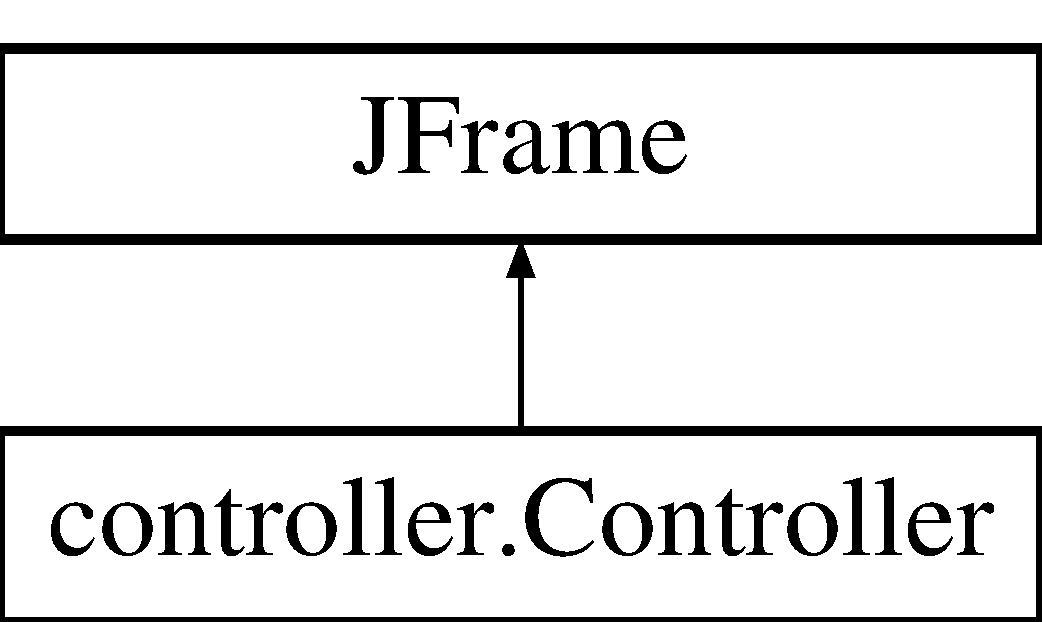
\includegraphics[height=2.000000cm]{classcontroller_1_1_controller}
\end{center}
\end{figure}
\subsection*{Public Member Functions}
\begin{DoxyCompactItemize}
\item 
\mbox{\Hypertarget{classcontroller_1_1_controller_adec12cce695b249689e63a10d307e2fe}\label{classcontroller_1_1_controller_adec12cce695b249689e63a10d307e2fe}} 
{\bfseries Controller} (\mbox{\hyperlink{class_g_u_i_1_1_main}{Main}} main, boolean custom\+Mode)
\item 
void \mbox{\hyperlink{classcontroller_1_1_controller_aef977092ec31c33e0f76ced1d3b55647}{restart\+Game}} ()
\item 
void \mbox{\hyperlink{classcontroller_1_1_controller_ab82a41df79bac7338424998579c31729}{forfeit}} ()
\item 
void \mbox{\hyperlink{classcontroller_1_1_controller_a4e937aa816be2e00cc7ae10836c6aa13}{unique\+Name}} ()
\item 
void \mbox{\hyperlink{classcontroller_1_1_controller_a887f5b6788ff3f0001cf02d7ba5e6b27}{undo}} ()
\end{DoxyCompactItemize}
\subsection*{Public Attributes}
\begin{DoxyCompactItemize}
\item 
\mbox{\Hypertarget{classcontroller_1_1_controller_a3d56c576c4f3a12e8abfddc9a69fd994}\label{classcontroller_1_1_controller_a3d56c576c4f3a12e8abfddc9a69fd994}} 
\mbox{\hyperlink{classmain_1_1_board}{Board}} {\bfseries board}
\item 
\mbox{\Hypertarget{classcontroller_1_1_controller_a331e08373c3c83fce5e754a385f1ee69}\label{classcontroller_1_1_controller_a331e08373c3c83fce5e754a385f1ee69}} 
\mbox{\hyperlink{class_g_u_i_1_1_g_u_i_board}{G\+U\+I\+Board}} {\bfseries gui\+Board}
\item 
\mbox{\Hypertarget{classcontroller_1_1_controller_a15d46dfda0e4e828b1196912a8d93821}\label{classcontroller_1_1_controller_a15d46dfda0e4e828b1196912a8d93821}} 
\mbox{\hyperlink{class_g_u_i_1_1_main}{Main}} {\bfseries main\+Window}
\item 
\mbox{\Hypertarget{classcontroller_1_1_controller_a277855441c2d9125f1c872ee9d03b18b}\label{classcontroller_1_1_controller_a277855441c2d9125f1c872ee9d03b18b}} 
int {\bfseries score1}
\item 
\mbox{\Hypertarget{classcontroller_1_1_controller_a808e7e0237d13d4607c1cc5aaebc67e2}\label{classcontroller_1_1_controller_a808e7e0237d13d4607c1cc5aaebc67e2}} 
int {\bfseries score2}
\item 
\mbox{\Hypertarget{classcontroller_1_1_controller_a155aee4f56e6261e91f480d9275805ac}\label{classcontroller_1_1_controller_a155aee4f56e6261e91f480d9275805ac}} 
boolean {\bfseries custom\+Mode}
\item 
\mbox{\Hypertarget{classcontroller_1_1_controller_a71e422cd3e140bd6c7ce4f556c8ad67e}\label{classcontroller_1_1_controller_a71e422cd3e140bd6c7ce4f556c8ad67e}} 
String {\bfseries black\+Name}
\item 
\mbox{\Hypertarget{classcontroller_1_1_controller_ac76189cee454bed016a8484a0c325312}\label{classcontroller_1_1_controller_ac76189cee454bed016a8484a0c325312}} 
String {\bfseries white\+Name}
\end{DoxyCompactItemize}


\subsection{Member Function Documentation}
\mbox{\Hypertarget{classcontroller_1_1_controller_ab82a41df79bac7338424998579c31729}\label{classcontroller_1_1_controller_ab82a41df79bac7338424998579c31729}} 
\index{controller\+::\+Controller@{controller\+::\+Controller}!forfeit@{forfeit}}
\index{forfeit@{forfeit}!controller\+::\+Controller@{controller\+::\+Controller}}
\subsubsection{\texorpdfstring{forfeit()}{forfeit()}}
{\footnotesize\ttfamily void controller.\+Controller.\+forfeit (\begin{DoxyParamCaption}{ }\end{DoxyParamCaption})\hspace{0.3cm}{\ttfamily [inline]}}

forfeit function \mbox{\Hypertarget{classcontroller_1_1_controller_aef977092ec31c33e0f76ced1d3b55647}\label{classcontroller_1_1_controller_aef977092ec31c33e0f76ced1d3b55647}} 
\index{controller\+::\+Controller@{controller\+::\+Controller}!restart\+Game@{restart\+Game}}
\index{restart\+Game@{restart\+Game}!controller\+::\+Controller@{controller\+::\+Controller}}
\subsubsection{\texorpdfstring{restart\+Game()}{restartGame()}}
{\footnotesize\ttfamily void controller.\+Controller.\+restart\+Game (\begin{DoxyParamCaption}{ }\end{DoxyParamCaption})\hspace{0.3cm}{\ttfamily [inline]}}

restart the gmae \mbox{\Hypertarget{classcontroller_1_1_controller_a887f5b6788ff3f0001cf02d7ba5e6b27}\label{classcontroller_1_1_controller_a887f5b6788ff3f0001cf02d7ba5e6b27}} 
\index{controller\+::\+Controller@{controller\+::\+Controller}!undo@{undo}}
\index{undo@{undo}!controller\+::\+Controller@{controller\+::\+Controller}}
\subsubsection{\texorpdfstring{undo()}{undo()}}
{\footnotesize\ttfamily void controller.\+Controller.\+undo (\begin{DoxyParamCaption}{ }\end{DoxyParamCaption})\hspace{0.3cm}{\ttfamily [inline]}}

undo in both gui and board structure \mbox{\Hypertarget{classcontroller_1_1_controller_a4e937aa816be2e00cc7ae10836c6aa13}\label{classcontroller_1_1_controller_a4e937aa816be2e00cc7ae10836c6aa13}} 
\index{controller\+::\+Controller@{controller\+::\+Controller}!unique\+Name@{unique\+Name}}
\index{unique\+Name@{unique\+Name}!controller\+::\+Controller@{controller\+::\+Controller}}
\subsubsection{\texorpdfstring{unique\+Name()}{uniqueName()}}
{\footnotesize\ttfamily void controller.\+Controller.\+unique\+Name (\begin{DoxyParamCaption}{ }\end{DoxyParamCaption})\hspace{0.3cm}{\ttfamily [inline]}}

let user type in their name 

The documentation for this class was generated from the following file\+:\begin{DoxyCompactItemize}
\item 
controller/Controller.\+java\end{DoxyCompactItemize}

\hypertarget{classmain_1_1_crab}{}\section{main.\+Crab Class Reference}
\label{classmain_1_1_crab}\index{main.\+Crab@{main.\+Crab}}
Inheritance diagram for main.\+Crab\+:\begin{figure}[H]
\begin{center}
\leavevmode
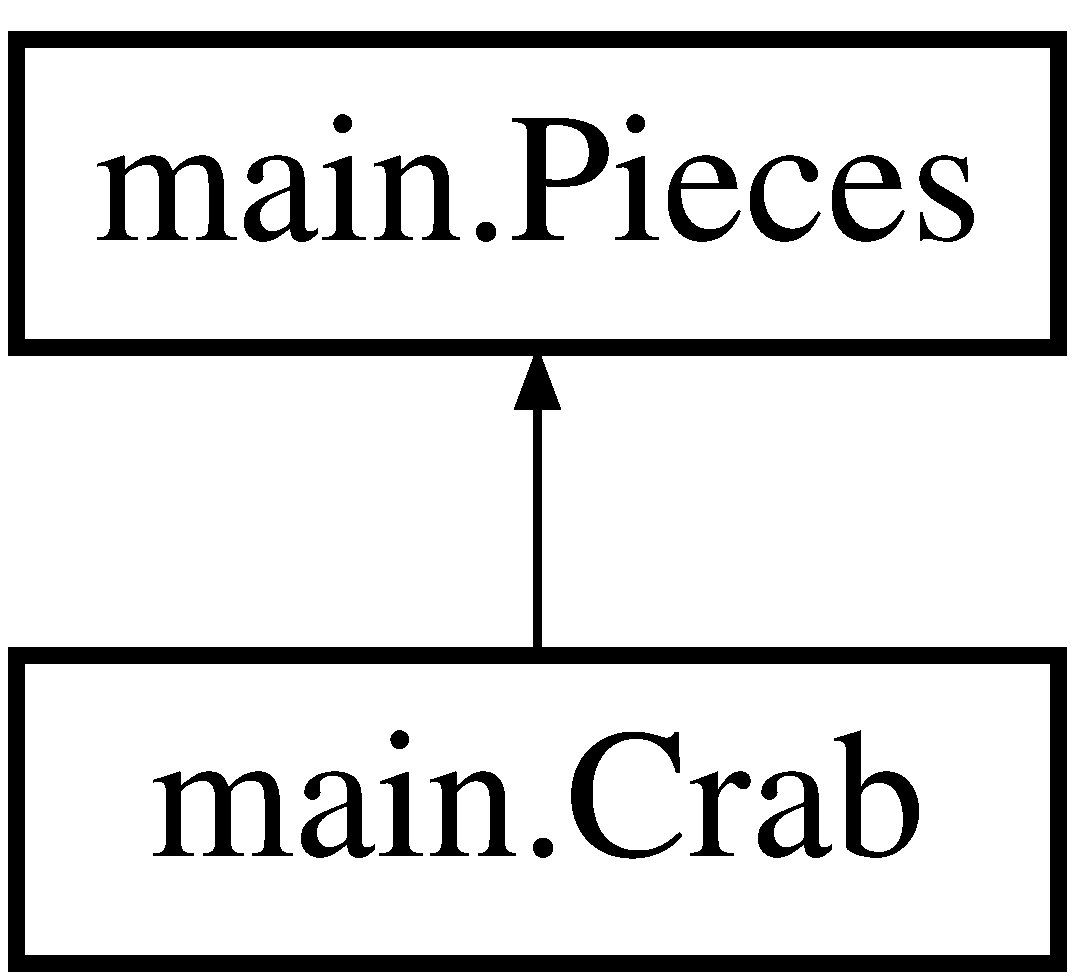
\includegraphics[height=2.000000cm]{classmain_1_1_crab}
\end{center}
\end{figure}
\subsection*{Public Member Functions}
\begin{DoxyCompactItemize}
\item 
\mbox{\hyperlink{classmain_1_1_crab_a99412eb33f8d2d50f338381651d2228f}{Crab}} (int x, int y, int player)
\item 
boolean \mbox{\hyperlink{classmain_1_1_crab_a386a6f3c85fcaf998971570aeb9ea193}{is\+Valid\+Move}} (int newX, int newY)
\item 
boolean \mbox{\hyperlink{classmain_1_1_crab_a726d4e88d2f0e4942ed47ff40539974e}{valid\+Move}} (int newX, int newY, \mbox{\hyperlink{classmain_1_1_board}{Board}} board)
\item 
boolean \mbox{\hyperlink{classmain_1_1_crab_ac72368c64c168408bb92132db1119b31}{could\+Be\+Stopped}} (int newX, int newY, \mbox{\hyperlink{classmain_1_1_board}{Board}} board)
\item 
boolean \mbox{\hyperlink{classmain_1_1_crab_acc3712804963dc82ffc3f155f8753b41}{is\+Movable}} (\mbox{\hyperlink{classmain_1_1_board}{Board}} board)
\end{DoxyCompactItemize}
\subsection*{Additional Inherited Members}


\subsection{Detailed Description}
\begin{DoxyAuthor}{Author}
kaichenle 
\end{DoxyAuthor}


\subsection{Constructor \& Destructor Documentation}
\mbox{\Hypertarget{classmain_1_1_crab_a99412eb33f8d2d50f338381651d2228f}\label{classmain_1_1_crab_a99412eb33f8d2d50f338381651d2228f}} 
\index{main\+::\+Crab@{main\+::\+Crab}!Crab@{Crab}}
\index{Crab@{Crab}!main\+::\+Crab@{main\+::\+Crab}}
\subsubsection{\texorpdfstring{Crab()}{Crab()}}
{\footnotesize\ttfamily main.\+Crab.\+Crab (\begin{DoxyParamCaption}\item[{int}]{x,  }\item[{int}]{y,  }\item[{int}]{player }\end{DoxyParamCaption})\hspace{0.3cm}{\ttfamily [inline]}}

constructor 
\begin{DoxyParams}{Parameters}
{\em x} & x\+Coord \\
\hline
{\em y} & y\+Coord \\
\hline
{\em player} & player 1 or 2 \\
\hline
\end{DoxyParams}


\subsection{Member Function Documentation}
\mbox{\Hypertarget{classmain_1_1_crab_ac72368c64c168408bb92132db1119b31}\label{classmain_1_1_crab_ac72368c64c168408bb92132db1119b31}} 
\index{main\+::\+Crab@{main\+::\+Crab}!could\+Be\+Stopped@{could\+Be\+Stopped}}
\index{could\+Be\+Stopped@{could\+Be\+Stopped}!main\+::\+Crab@{main\+::\+Crab}}
\subsubsection{\texorpdfstring{could\+Be\+Stopped()}{couldBeStopped()}}
{\footnotesize\ttfamily boolean main.\+Crab.\+could\+Be\+Stopped (\begin{DoxyParamCaption}\item[{int}]{newX,  }\item[{int}]{newY,  }\item[{\mbox{\hyperlink{classmain_1_1_board}{Board}}}]{board }\end{DoxyParamCaption})\hspace{0.3cm}{\ttfamily [inline]}}

if any pieces could stop input \mbox{\hyperlink{classmain_1_1_crab}{Crab}} piece from x,y to newX newY 
\begin{DoxyParams}{Parameters}
{\em newX} & end x\+Coord \\
\hline
{\em newY} & end y\+Coord \\
\hline
{\em board} & that the chess play on \\
\hline
\end{DoxyParams}
\begin{DoxyReturn}{Returns}
true if there is a piece exists that can stop the chess otherwise false 
\end{DoxyReturn}
\mbox{\Hypertarget{classmain_1_1_crab_acc3712804963dc82ffc3f155f8753b41}\label{classmain_1_1_crab_acc3712804963dc82ffc3f155f8753b41}} 
\index{main\+::\+Crab@{main\+::\+Crab}!is\+Movable@{is\+Movable}}
\index{is\+Movable@{is\+Movable}!main\+::\+Crab@{main\+::\+Crab}}
\subsubsection{\texorpdfstring{is\+Movable()}{isMovable()}}
{\footnotesize\ttfamily boolean main.\+Crab.\+is\+Movable (\begin{DoxyParamCaption}\item[{\mbox{\hyperlink{classmain_1_1_board}{Board}}}]{board }\end{DoxyParamCaption})\hspace{0.3cm}{\ttfamily [inline]}}

helper functions check movability of \mbox{\hyperlink{classmain_1_1_crab}{Crab}} 
\begin{DoxyParams}{Parameters}
{\em board} & the game will be on \\
\hline
\end{DoxyParams}
\begin{DoxyReturn}{Returns}
true if the input can move otherwise false 
\end{DoxyReturn}
\mbox{\Hypertarget{classmain_1_1_crab_a386a6f3c85fcaf998971570aeb9ea193}\label{classmain_1_1_crab_a386a6f3c85fcaf998971570aeb9ea193}} 
\index{main\+::\+Crab@{main\+::\+Crab}!is\+Valid\+Move@{is\+Valid\+Move}}
\index{is\+Valid\+Move@{is\+Valid\+Move}!main\+::\+Crab@{main\+::\+Crab}}
\subsubsection{\texorpdfstring{is\+Valid\+Move()}{isValidMove()}}
{\footnotesize\ttfamily boolean main.\+Crab.\+is\+Valid\+Move (\begin{DoxyParamCaption}\item[{int}]{newX,  }\item[{int}]{newY }\end{DoxyParamCaption})\hspace{0.3cm}{\ttfamily [inline]}}

see if the chess move against convention without consider other chesses \mbox{\Hypertarget{classmain_1_1_crab_a726d4e88d2f0e4942ed47ff40539974e}\label{classmain_1_1_crab_a726d4e88d2f0e4942ed47ff40539974e}} 
\index{main\+::\+Crab@{main\+::\+Crab}!valid\+Move@{valid\+Move}}
\index{valid\+Move@{valid\+Move}!main\+::\+Crab@{main\+::\+Crab}}
\subsubsection{\texorpdfstring{valid\+Move()}{validMove()}}
{\footnotesize\ttfamily boolean main.\+Crab.\+valid\+Move (\begin{DoxyParamCaption}\item[{int}]{newX,  }\item[{int}]{newY,  }\item[{\mbox{\hyperlink{classmain_1_1_board}{Board}}}]{board }\end{DoxyParamCaption})\hspace{0.3cm}{\ttfamily [inline]}}

Helper functions check if it is a valid path to move \mbox{\hyperlink{classmain_1_1_crab}{Crab}}. It will be called inside move\+Chess with is\+Valid\+Move in each pieces subclass. This will check if there are pieces on the board that will influence the fact if it is valid to move chess 
\begin{DoxyParams}{Parameters}
{\em newX} & end y\+Coord \\
\hline
{\em newY} & end y\+Coord \\
\hline
{\em board} & the chess play on \\
\hline
\end{DoxyParams}
\begin{DoxyReturn}{Returns}
true if valid otherwise false 
\end{DoxyReturn}


The documentation for this class was generated from the following file\+:\begin{DoxyCompactItemize}
\item 
main/Crab.\+java\end{DoxyCompactItemize}

\hypertarget{classtests_1_1_crab_tests}{}\section{tests.\+Crab\+Tests Class Reference}
\label{classtests_1_1_crab_tests}\index{tests.\+Crab\+Tests@{tests.\+Crab\+Tests}}
\subsection*{Public Member Functions}
\begin{DoxyCompactItemize}
\item 
\mbox{\Hypertarget{classtests_1_1_crab_tests_a993d6a9afed7b341bca83836f49bf602}\label{classtests_1_1_crab_tests_a993d6a9afed7b341bca83836f49bf602}} 
void {\bfseries should\+Move\+Crab} ()
\item 
void \mbox{\hyperlink{classtests_1_1_crab_tests_a995106565f790757dd5df4619ba84d97}{is\+Movable\+Crab}} ()
\item 
\mbox{\Hypertarget{classtests_1_1_crab_tests_a2177db7c9a4d5c05f6499180f8bb4a66}\label{classtests_1_1_crab_tests_a2177db7c9a4d5c05f6499180f8bb4a66}} 
void {\bfseries could\+Be\+Stopped\+Ox} ()
\end{DoxyCompactItemize}


\subsection{Member Function Documentation}
\mbox{\Hypertarget{classtests_1_1_crab_tests_a995106565f790757dd5df4619ba84d97}\label{classtests_1_1_crab_tests_a995106565f790757dd5df4619ba84d97}} 
\index{tests\+::\+Crab\+Tests@{tests\+::\+Crab\+Tests}!is\+Movable\+Crab@{is\+Movable\+Crab}}
\index{is\+Movable\+Crab@{is\+Movable\+Crab}!tests\+::\+Crab\+Tests@{tests\+::\+Crab\+Tests}}
\subsubsection{\texorpdfstring{is\+Movable\+Crab()}{isMovableCrab()}}
{\footnotesize\ttfamily void tests.\+Crab\+Tests.\+is\+Movable\+Crab (\begin{DoxyParamCaption}{ }\end{DoxyParamCaption})\hspace{0.3cm}{\ttfamily [inline]}}

test on is\+Movable 

The documentation for this class was generated from the following file\+:\begin{DoxyCompactItemize}
\item 
tests/Crab\+Tests.\+java\end{DoxyCompactItemize}

\hypertarget{class_g_u_i_1_1_g_u_i_board}{}\section{G\+U\+I.\+G\+U\+I\+Board Class Reference}
\label{class_g_u_i_1_1_g_u_i_board}\index{G\+U\+I.\+G\+U\+I\+Board@{G\+U\+I.\+G\+U\+I\+Board}}
\subsection*{Classes}
\begin{DoxyCompactItemize}
\item 
class \mbox{\hyperlink{class_g_u_i_1_1_g_u_i_board_1_1_table}{Table}}
\end{DoxyCompactItemize}
\subsection*{Public Member Functions}
\begin{DoxyCompactItemize}
\item 
\mbox{\Hypertarget{class_g_u_i_1_1_g_u_i_board_a1120e559dc54adc2935d4e342dafc1f6}\label{class_g_u_i_1_1_g_u_i_board_a1120e559dc54adc2935d4e342dafc1f6}} 
{\bfseries G\+U\+I\+Board} (\mbox{\hyperlink{class_g_u_i_1_1_main}{Main}} main)
\end{DoxyCompactItemize}
\subsection*{Public Attributes}
\begin{DoxyCompactItemize}
\item 
\mbox{\Hypertarget{class_g_u_i_1_1_g_u_i_board_a4249ff44b1425772cd7745daa8a65502}\label{class_g_u_i_1_1_g_u_i_board_a4249ff44b1425772cd7745daa8a65502}} 
int {\bfseries offset\+Interval}
\item 
\mbox{\Hypertarget{class_g_u_i_1_1_g_u_i_board_a58264f7aadfc39c69c895d8eb8ec785a}\label{class_g_u_i_1_1_g_u_i_board_a58264f7aadfc39c69c895d8eb8ec785a}} 
J\+Button {\bfseries chess\+To\+Be\+Moved}
\item 
\mbox{\Hypertarget{class_g_u_i_1_1_g_u_i_board_aff10adcc6704200b4c99ec555ac5d2b7}\label{class_g_u_i_1_1_g_u_i_board_aff10adcc6704200b4c99ec555ac5d2b7}} 
\mbox{\hyperlink{classcontroller_1_1_controller}{Controller}} {\bfseries controller}
\item 
\mbox{\Hypertarget{class_g_u_i_1_1_g_u_i_board_a90cb8a48e91297887da1f7a4d662379d}\label{class_g_u_i_1_1_g_u_i_board_a90cb8a48e91297887da1f7a4d662379d}} 
Stack$<$ J\+Button $>$ {\bfseries black\+Past}
\item 
\mbox{\Hypertarget{class_g_u_i_1_1_g_u_i_board_a62c92e6bcb1af75e736430618eed1044}\label{class_g_u_i_1_1_g_u_i_board_a62c92e6bcb1af75e736430618eed1044}} 
Stack$<$ J\+Button $>$ {\bfseries white\+Past}
\item 
\mbox{\Hypertarget{class_g_u_i_1_1_g_u_i_board_ade0e86075ec61020a8fdbe82a196b1f8}\label{class_g_u_i_1_1_g_u_i_board_ade0e86075ec61020a8fdbe82a196b1f8}} 
J\+Button {\bfseries black\+Start}
\item 
\mbox{\Hypertarget{class_g_u_i_1_1_g_u_i_board_a372138442699ff3637eabdc2cd91a41a}\label{class_g_u_i_1_1_g_u_i_board_a372138442699ff3637eabdc2cd91a41a}} 
J\+Button {\bfseries black\+End}
\item 
\mbox{\Hypertarget{class_g_u_i_1_1_g_u_i_board_a6763993686c9cffa1eb91bd125eef9b1}\label{class_g_u_i_1_1_g_u_i_board_a6763993686c9cffa1eb91bd125eef9b1}} 
J\+Button {\bfseries white\+Start}
\item 
\mbox{\Hypertarget{class_g_u_i_1_1_g_u_i_board_a6235dad380ee6ce06d2ed15dadd5ee9a}\label{class_g_u_i_1_1_g_u_i_board_a6235dad380ee6ce06d2ed15dadd5ee9a}} 
J\+Button {\bfseries white\+End}
\item 
\mbox{\Hypertarget{class_g_u_i_1_1_g_u_i_board_a80bc71dfcf0e8e4e13d28c8eb4e17ae7}\label{class_g_u_i_1_1_g_u_i_board_a80bc71dfcf0e8e4e13d28c8eb4e17ae7}} 
\mbox{\hyperlink{class_g_u_i_1_1_g_u_i_board_1_1_table}{Table}} {\bfseries table}
\end{DoxyCompactItemize}


The documentation for this class was generated from the following file\+:\begin{DoxyCompactItemize}
\item 
G\+U\+I/G\+U\+I\+Board.\+java\end{DoxyCompactItemize}

\hypertarget{class_g_u_i_1_1_g_u_i_menu}{}\section{G\+U\+I.\+G\+U\+I\+Menu Class Reference}
\label{class_g_u_i_1_1_g_u_i_menu}\index{G\+U\+I.\+G\+U\+I\+Menu@{G\+U\+I.\+G\+U\+I\+Menu}}
Inheritance diagram for G\+U\+I.\+G\+U\+I\+Menu\+:\begin{figure}[H]
\begin{center}
\leavevmode
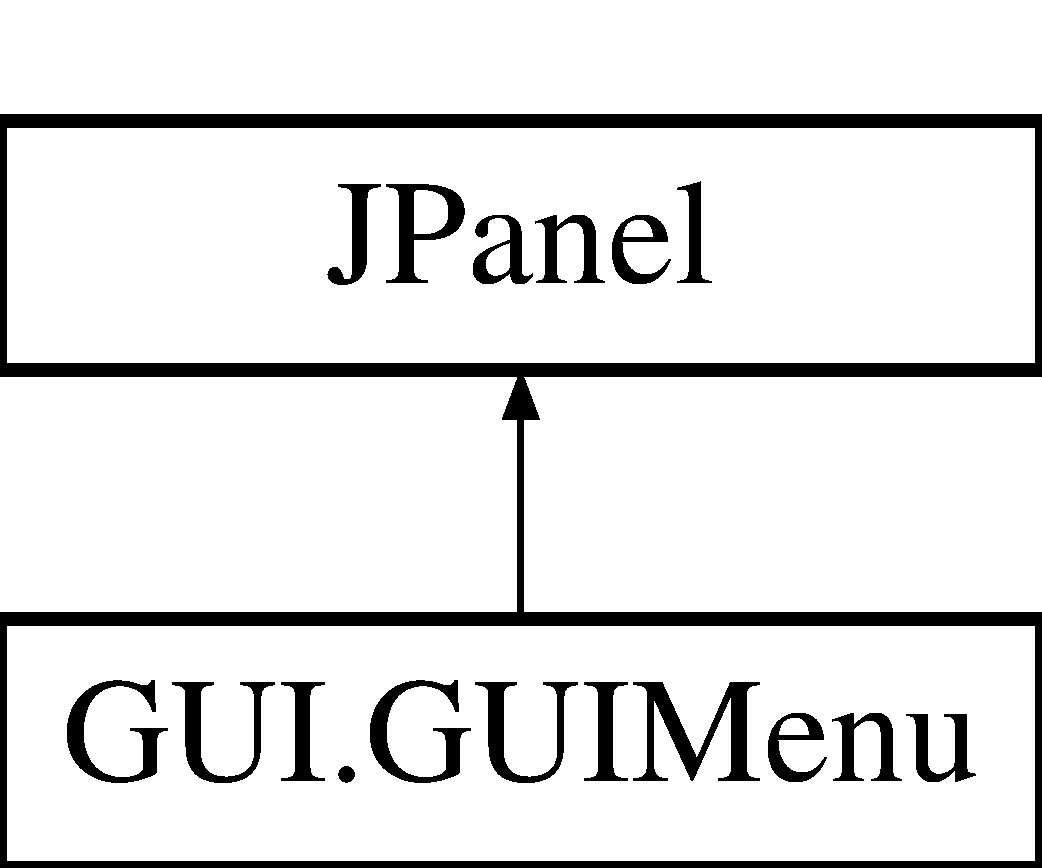
\includegraphics[height=2.000000cm]{class_g_u_i_1_1_g_u_i_menu}
\end{center}
\end{figure}
\subsection*{Public Member Functions}
\begin{DoxyCompactItemize}
\item 
\mbox{\Hypertarget{class_g_u_i_1_1_g_u_i_menu_a3b45d110394a3f206e2b559ee21fdf36}\label{class_g_u_i_1_1_g_u_i_menu_a3b45d110394a3f206e2b559ee21fdf36}} 
{\bfseries G\+U\+I\+Menu} (\mbox{\hyperlink{class_g_u_i_1_1_main}{Main}} main)
\item 
\mbox{\Hypertarget{class_g_u_i_1_1_g_u_i_menu_a5591425611de8bef9f7d8e08f07df713}\label{class_g_u_i_1_1_g_u_i_menu_a5591425611de8bef9f7d8e08f07df713}} 
void {\bfseries set\+Score} (String white\+Name, String black\+Name, int black\+Score, int white\+Score)
\end{DoxyCompactItemize}
\subsection*{Public Attributes}
\begin{DoxyCompactItemize}
\item 
\mbox{\Hypertarget{class_g_u_i_1_1_g_u_i_menu_a3dd67b46f7aa24b23a605fa542459433}\label{class_g_u_i_1_1_g_u_i_menu_a3dd67b46f7aa24b23a605fa542459433}} 
J\+Label {\bfseries white}
\item 
\mbox{\Hypertarget{class_g_u_i_1_1_g_u_i_menu_a0f6d24966fb59fc6521f1d0db2af68f4}\label{class_g_u_i_1_1_g_u_i_menu_a0f6d24966fb59fc6521f1d0db2af68f4}} 
J\+Label {\bfseries black}
\end{DoxyCompactItemize}


The documentation for this class was generated from the following file\+:\begin{DoxyCompactItemize}
\item 
G\+U\+I/G\+U\+I\+Menu.\+java\end{DoxyCompactItemize}

\hypertarget{classmain_1_1_king}{}\section{main.\+King Class Reference}
\label{classmain_1_1_king}\index{main.\+King@{main.\+King}}
Inheritance diagram for main.\+King\+:\begin{figure}[H]
\begin{center}
\leavevmode
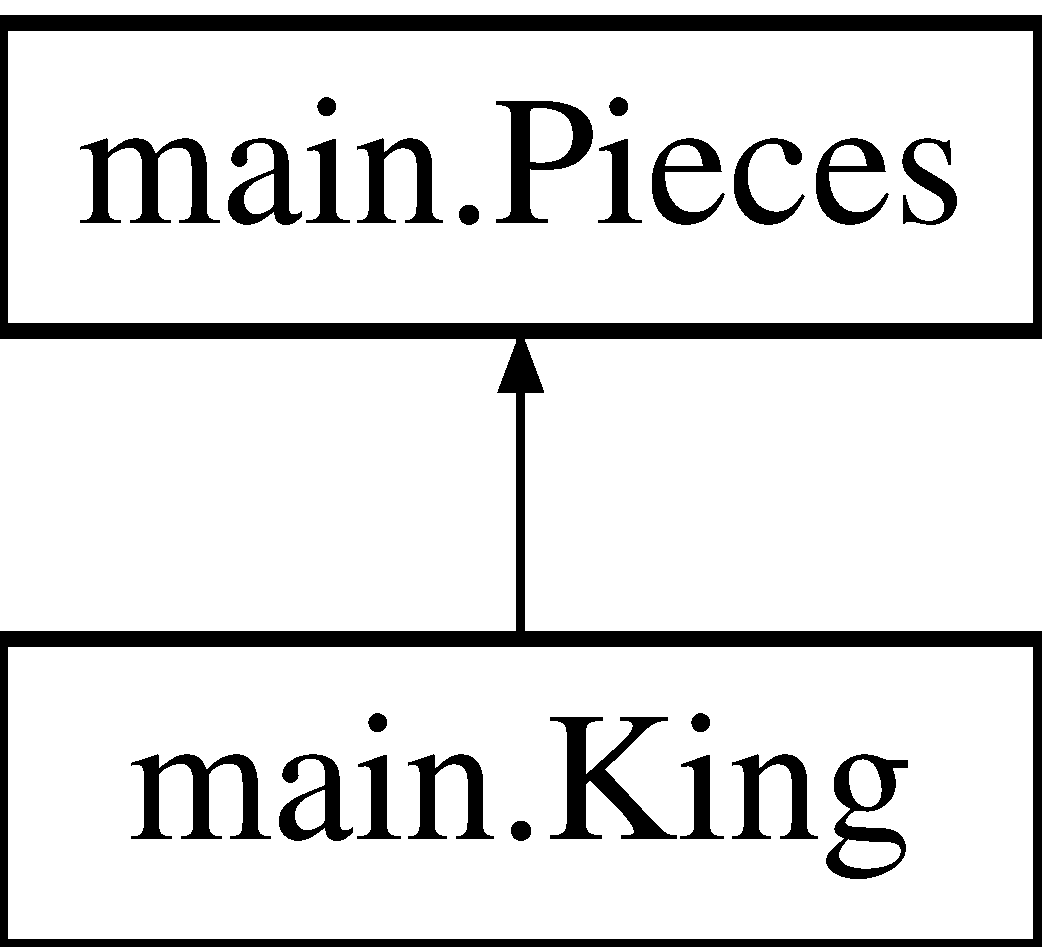
\includegraphics[height=2.000000cm]{classmain_1_1_king}
\end{center}
\end{figure}
\subsection*{Public Member Functions}
\begin{DoxyCompactItemize}
\item 
\mbox{\hyperlink{classmain_1_1_king_ae513926e77ae13577530d820c400e6f3}{King}} (int x, int y, int player)
\item 
boolean \mbox{\hyperlink{classmain_1_1_king_ac7fc89ee4c93a500d49ec3dede5282d6}{is\+Valid\+Move}} (int newX, int newY)
\item 
boolean \mbox{\hyperlink{classmain_1_1_king_af01e8aeb9a6a32c89b0b60d47a90232b}{valid\+Move}} (int newX, int newY, \mbox{\hyperlink{classmain_1_1_board}{Board}} board)
\item 
boolean \mbox{\hyperlink{classmain_1_1_king_ab04709bedac4618b9683cb09dc0dbdc3}{could\+Be\+Stopped}} (int newX, int newY, \mbox{\hyperlink{classmain_1_1_board}{Board}} board)
\item 
boolean \mbox{\hyperlink{classmain_1_1_king_a30d717327a122f2ef2e07760914c5e33}{is\+Movable}} (\mbox{\hyperlink{classmain_1_1_board}{Board}} board)
\end{DoxyCompactItemize}
\subsection*{Additional Inherited Members}


\subsection{Detailed Description}
\begin{DoxyAuthor}{Author}
kaichenle 
\end{DoxyAuthor}


\subsection{Constructor \& Destructor Documentation}
\mbox{\Hypertarget{classmain_1_1_king_ae513926e77ae13577530d820c400e6f3}\label{classmain_1_1_king_ae513926e77ae13577530d820c400e6f3}} 
\index{main\+::\+King@{main\+::\+King}!King@{King}}
\index{King@{King}!main\+::\+King@{main\+::\+King}}
\subsubsection{\texorpdfstring{King()}{King()}}
{\footnotesize\ttfamily main.\+King.\+King (\begin{DoxyParamCaption}\item[{int}]{x,  }\item[{int}]{y,  }\item[{int}]{player }\end{DoxyParamCaption})\hspace{0.3cm}{\ttfamily [inline]}}

constructor 
\begin{DoxyParams}{Parameters}
{\em x} & x\+Coord \\
\hline
{\em y} & y\+Coord \\
\hline
{\em player} & player 1 or 2 \\
\hline
\end{DoxyParams}


\subsection{Member Function Documentation}
\mbox{\Hypertarget{classmain_1_1_king_ab04709bedac4618b9683cb09dc0dbdc3}\label{classmain_1_1_king_ab04709bedac4618b9683cb09dc0dbdc3}} 
\index{main\+::\+King@{main\+::\+King}!could\+Be\+Stopped@{could\+Be\+Stopped}}
\index{could\+Be\+Stopped@{could\+Be\+Stopped}!main\+::\+King@{main\+::\+King}}
\subsubsection{\texorpdfstring{could\+Be\+Stopped()}{couldBeStopped()}}
{\footnotesize\ttfamily boolean main.\+King.\+could\+Be\+Stopped (\begin{DoxyParamCaption}\item[{int}]{newX,  }\item[{int}]{newY,  }\item[{\mbox{\hyperlink{classmain_1_1_board}{Board}}}]{board }\end{DoxyParamCaption})\hspace{0.3cm}{\ttfamily [inline]}}

if any pieces could stop input bishop or queen(diaganol) piece from x,y to newX newY 
\begin{DoxyParams}{Parameters}
{\em newX} & end x\+Coord \\
\hline
{\em newY} & end y\+Coord \\
\hline
{\em board} & the game will play on \\
\hline
\end{DoxyParams}
\begin{DoxyReturn}{Returns}
true if there is a piece exists otherwise false 
\end{DoxyReturn}
\mbox{\Hypertarget{classmain_1_1_king_a30d717327a122f2ef2e07760914c5e33}\label{classmain_1_1_king_a30d717327a122f2ef2e07760914c5e33}} 
\index{main\+::\+King@{main\+::\+King}!is\+Movable@{is\+Movable}}
\index{is\+Movable@{is\+Movable}!main\+::\+King@{main\+::\+King}}
\subsubsection{\texorpdfstring{is\+Movable()}{isMovable()}}
{\footnotesize\ttfamily boolean main.\+King.\+is\+Movable (\begin{DoxyParamCaption}\item[{\mbox{\hyperlink{classmain_1_1_board}{Board}}}]{board }\end{DoxyParamCaption})\hspace{0.3cm}{\ttfamily [inline]}}

helper functions check movability of bishop or queen(diaganol) 
\begin{DoxyParams}{Parameters}
{\em board} & the game will be on \\
\hline
\end{DoxyParams}
\begin{DoxyReturn}{Returns}
true if the input can move otherwise false 
\end{DoxyReturn}
\mbox{\Hypertarget{classmain_1_1_king_ac7fc89ee4c93a500d49ec3dede5282d6}\label{classmain_1_1_king_ac7fc89ee4c93a500d49ec3dede5282d6}} 
\index{main\+::\+King@{main\+::\+King}!is\+Valid\+Move@{is\+Valid\+Move}}
\index{is\+Valid\+Move@{is\+Valid\+Move}!main\+::\+King@{main\+::\+King}}
\subsubsection{\texorpdfstring{is\+Valid\+Move()}{isValidMove()}}
{\footnotesize\ttfamily boolean main.\+King.\+is\+Valid\+Move (\begin{DoxyParamCaption}\item[{int}]{newX,  }\item[{int}]{newY }\end{DoxyParamCaption})\hspace{0.3cm}{\ttfamily [inline]}}

see if the chess move against convention without consider other chesses \mbox{\Hypertarget{classmain_1_1_king_af01e8aeb9a6a32c89b0b60d47a90232b}\label{classmain_1_1_king_af01e8aeb9a6a32c89b0b60d47a90232b}} 
\index{main\+::\+King@{main\+::\+King}!valid\+Move@{valid\+Move}}
\index{valid\+Move@{valid\+Move}!main\+::\+King@{main\+::\+King}}
\subsubsection{\texorpdfstring{valid\+Move()}{validMove()}}
{\footnotesize\ttfamily boolean main.\+King.\+valid\+Move (\begin{DoxyParamCaption}\item[{int}]{newX,  }\item[{int}]{newY,  }\item[{\mbox{\hyperlink{classmain_1_1_board}{Board}}}]{board }\end{DoxyParamCaption})\hspace{0.3cm}{\ttfamily [inline]}}

Helper functions check if it is a valid path to move king. It will be called inside move\+Chess with is\+Valid\+Move in each pieces subclass. This will check if there are pieces on the board that will influence the fact if it is valid to move chess 
\begin{DoxyParams}{Parameters}
{\em newX} & end y\+Coord \\
\hline
{\em newY} & end y\+Coord \\
\hline
{\em board} & the board the chess will play on \\
\hline
\end{DoxyParams}
\begin{DoxyReturn}{Returns}
true if valid otherwise false 
\end{DoxyReturn}


The documentation for this class was generated from the following file\+:\begin{DoxyCompactItemize}
\item 
main/King.\+java\end{DoxyCompactItemize}

\hypertarget{classtests_1_1_king_tests}{}\section{tests.\+King\+Tests Class Reference}
\label{classtests_1_1_king_tests}\index{tests.\+King\+Tests@{tests.\+King\+Tests}}
\subsection*{Public Member Functions}
\begin{DoxyCompactItemize}
\item 
void \mbox{\hyperlink{classtests_1_1_king_tests_a4a13975c203ea411af32909db0364f4c}{should\+Move\+King}} ()
\item 
\mbox{\Hypertarget{classtests_1_1_king_tests_a0e01efb662d38cd9537a1134b4600bcf}\label{classtests_1_1_king_tests_a0e01efb662d38cd9537a1134b4600bcf}} 
void {\bfseries is\+Movable\+King} ()
\end{DoxyCompactItemize}


\subsection{Detailed Description}
\begin{DoxyAuthor}{Author}
kaichenle 
\end{DoxyAuthor}


\subsection{Member Function Documentation}
\mbox{\Hypertarget{classtests_1_1_king_tests_a4a13975c203ea411af32909db0364f4c}\label{classtests_1_1_king_tests_a4a13975c203ea411af32909db0364f4c}} 
\index{tests\+::\+King\+Tests@{tests\+::\+King\+Tests}!should\+Move\+King@{should\+Move\+King}}
\index{should\+Move\+King@{should\+Move\+King}!tests\+::\+King\+Tests@{tests\+::\+King\+Tests}}
\subsubsection{\texorpdfstring{should\+Move\+King()}{shouldMoveKing()}}
{\footnotesize\ttfamily void tests.\+King\+Tests.\+should\+Move\+King (\begin{DoxyParamCaption}{ }\end{DoxyParamCaption})\hspace{0.3cm}{\ttfamily [inline]}}

test on move\+Chess 

The documentation for this class was generated from the following file\+:\begin{DoxyCompactItemize}
\item 
tests/King\+Tests.\+java\end{DoxyCompactItemize}

\hypertarget{classmain_1_1_knight}{}\section{main.\+Knight Class Reference}
\label{classmain_1_1_knight}\index{main.\+Knight@{main.\+Knight}}
Inheritance diagram for main.\+Knight\+:\begin{figure}[H]
\begin{center}
\leavevmode
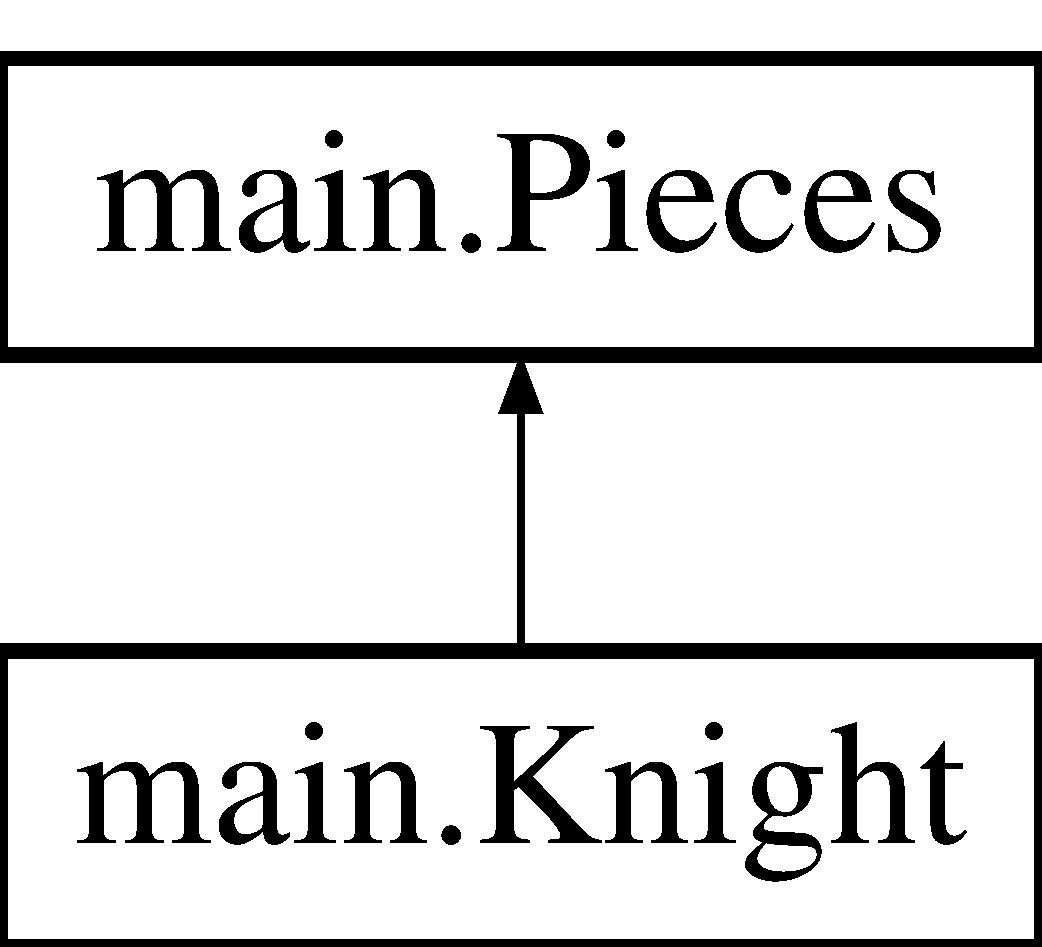
\includegraphics[height=2.000000cm]{classmain_1_1_knight}
\end{center}
\end{figure}
\subsection*{Public Member Functions}
\begin{DoxyCompactItemize}
\item 
\mbox{\hyperlink{classmain_1_1_knight_a57e9a5ff0ded3f5636fccf2325616837}{Knight}} (int x, int y, int player)
\item 
boolean \mbox{\hyperlink{classmain_1_1_knight_a65b314ba3dee673545222a60938d41ef}{is\+Valid\+Move}} (int newX, int newY)
\item 
boolean \mbox{\hyperlink{classmain_1_1_knight_a883345babf8f5cf09611ac25857939c6}{valid\+Move}} (int newX, int newY, \mbox{\hyperlink{classmain_1_1_board}{Board}} board)
\item 
boolean \mbox{\hyperlink{classmain_1_1_knight_a350832c72d961a9ddf0c4e4c1dcb4fae}{could\+Be\+Stopped}} (int newX, int newY, \mbox{\hyperlink{classmain_1_1_board}{Board}} board)
\item 
boolean \mbox{\hyperlink{classmain_1_1_knight_a1f2fc54af96bddbd4e06f1860f8c4a1e}{is\+Movable}} (\mbox{\hyperlink{classmain_1_1_board}{Board}} board)
\end{DoxyCompactItemize}
\subsection*{Additional Inherited Members}


\subsection{Detailed Description}
\begin{DoxyAuthor}{Author}
kaichenle 
\end{DoxyAuthor}


\subsection{Constructor \& Destructor Documentation}
\mbox{\Hypertarget{classmain_1_1_knight_a57e9a5ff0ded3f5636fccf2325616837}\label{classmain_1_1_knight_a57e9a5ff0ded3f5636fccf2325616837}} 
\index{main\+::\+Knight@{main\+::\+Knight}!Knight@{Knight}}
\index{Knight@{Knight}!main\+::\+Knight@{main\+::\+Knight}}
\subsubsection{\texorpdfstring{Knight()}{Knight()}}
{\footnotesize\ttfamily main.\+Knight.\+Knight (\begin{DoxyParamCaption}\item[{int}]{x,  }\item[{int}]{y,  }\item[{int}]{player }\end{DoxyParamCaption})\hspace{0.3cm}{\ttfamily [inline]}}

constructor 
\begin{DoxyParams}{Parameters}
{\em x} & x\+Coord \\
\hline
{\em y} & y\+Coord \\
\hline
{\em player} & player 1 or 2 \\
\hline
\end{DoxyParams}


\subsection{Member Function Documentation}
\mbox{\Hypertarget{classmain_1_1_knight_a350832c72d961a9ddf0c4e4c1dcb4fae}\label{classmain_1_1_knight_a350832c72d961a9ddf0c4e4c1dcb4fae}} 
\index{main\+::\+Knight@{main\+::\+Knight}!could\+Be\+Stopped@{could\+Be\+Stopped}}
\index{could\+Be\+Stopped@{could\+Be\+Stopped}!main\+::\+Knight@{main\+::\+Knight}}
\subsubsection{\texorpdfstring{could\+Be\+Stopped()}{couldBeStopped()}}
{\footnotesize\ttfamily boolean main.\+Knight.\+could\+Be\+Stopped (\begin{DoxyParamCaption}\item[{int}]{newX,  }\item[{int}]{newY,  }\item[{\mbox{\hyperlink{classmain_1_1_board}{Board}}}]{board }\end{DoxyParamCaption})\hspace{0.3cm}{\ttfamily [inline]}}

if any pieces could stop input bishop or queen(diaganol) piece from x,y to newX newY 
\begin{DoxyParams}{Parameters}
{\em newX} & end x\+Coord \\
\hline
{\em newY} & end y\+Coord \\
\hline
{\em board} & the game will play on \\
\hline
\end{DoxyParams}
\begin{DoxyReturn}{Returns}
true if there is a piece exists otherwise false 
\end{DoxyReturn}
\mbox{\Hypertarget{classmain_1_1_knight_a1f2fc54af96bddbd4e06f1860f8c4a1e}\label{classmain_1_1_knight_a1f2fc54af96bddbd4e06f1860f8c4a1e}} 
\index{main\+::\+Knight@{main\+::\+Knight}!is\+Movable@{is\+Movable}}
\index{is\+Movable@{is\+Movable}!main\+::\+Knight@{main\+::\+Knight}}
\subsubsection{\texorpdfstring{is\+Movable()}{isMovable()}}
{\footnotesize\ttfamily boolean main.\+Knight.\+is\+Movable (\begin{DoxyParamCaption}\item[{\mbox{\hyperlink{classmain_1_1_board}{Board}}}]{board }\end{DoxyParamCaption})\hspace{0.3cm}{\ttfamily [inline]}}

helper functions check movability of knight 
\begin{DoxyParams}{Parameters}
{\em board} & the game will play on \\
\hline
\end{DoxyParams}
\begin{DoxyReturn}{Returns}
true if the input can move otherwise false 
\end{DoxyReturn}
\mbox{\Hypertarget{classmain_1_1_knight_a65b314ba3dee673545222a60938d41ef}\label{classmain_1_1_knight_a65b314ba3dee673545222a60938d41ef}} 
\index{main\+::\+Knight@{main\+::\+Knight}!is\+Valid\+Move@{is\+Valid\+Move}}
\index{is\+Valid\+Move@{is\+Valid\+Move}!main\+::\+Knight@{main\+::\+Knight}}
\subsubsection{\texorpdfstring{is\+Valid\+Move()}{isValidMove()}}
{\footnotesize\ttfamily boolean main.\+Knight.\+is\+Valid\+Move (\begin{DoxyParamCaption}\item[{int}]{newX,  }\item[{int}]{newY }\end{DoxyParamCaption})\hspace{0.3cm}{\ttfamily [inline]}}

see if the chess move against convention without consider other chesses \mbox{\Hypertarget{classmain_1_1_knight_a883345babf8f5cf09611ac25857939c6}\label{classmain_1_1_knight_a883345babf8f5cf09611ac25857939c6}} 
\index{main\+::\+Knight@{main\+::\+Knight}!valid\+Move@{valid\+Move}}
\index{valid\+Move@{valid\+Move}!main\+::\+Knight@{main\+::\+Knight}}
\subsubsection{\texorpdfstring{valid\+Move()}{validMove()}}
{\footnotesize\ttfamily boolean main.\+Knight.\+valid\+Move (\begin{DoxyParamCaption}\item[{int}]{newX,  }\item[{int}]{newY,  }\item[{\mbox{\hyperlink{classmain_1_1_board}{Board}}}]{board }\end{DoxyParamCaption})\hspace{0.3cm}{\ttfamily [inline]}}

Helper functions check if it is a valid path to move knight. It will be called inside move\+Chess with is\+Valid\+Move in each pieces subclass. This will check if there are pieces on the board that will influence the fact if it is valid to move chess 
\begin{DoxyParams}{Parameters}
{\em newX} & end y\+Coord \\
\hline
{\em newY} & end y\+Coord \\
\hline
{\em board} & the chess will play on \\
\hline
\end{DoxyParams}
\begin{DoxyReturn}{Returns}
true if valid otherwise false 
\end{DoxyReturn}


The documentation for this class was generated from the following file\+:\begin{DoxyCompactItemize}
\item 
main/Knight.\+java\end{DoxyCompactItemize}

\hypertarget{classtests_1_1_knight_tests}{}\section{tests.\+Knight\+Tests Class Reference}
\label{classtests_1_1_knight_tests}\index{tests.\+Knight\+Tests@{tests.\+Knight\+Tests}}
\subsection*{Public Member Functions}
\begin{DoxyCompactItemize}
\item 
void \mbox{\hyperlink{classtests_1_1_knight_tests_ac21f03b73fc71f1a1042978344690cb7}{should\+Move\+Knight}} ()
\end{DoxyCompactItemize}


\subsection{Detailed Description}
\begin{DoxyAuthor}{Author}
kaichenle 
\end{DoxyAuthor}


\subsection{Member Function Documentation}
\mbox{\Hypertarget{classtests_1_1_knight_tests_ac21f03b73fc71f1a1042978344690cb7}\label{classtests_1_1_knight_tests_ac21f03b73fc71f1a1042978344690cb7}} 
\index{tests\+::\+Knight\+Tests@{tests\+::\+Knight\+Tests}!should\+Move\+Knight@{should\+Move\+Knight}}
\index{should\+Move\+Knight@{should\+Move\+Knight}!tests\+::\+Knight\+Tests@{tests\+::\+Knight\+Tests}}
\subsubsection{\texorpdfstring{should\+Move\+Knight()}{shouldMoveKnight()}}
{\footnotesize\ttfamily void tests.\+Knight\+Tests.\+should\+Move\+Knight (\begin{DoxyParamCaption}{ }\end{DoxyParamCaption})\hspace{0.3cm}{\ttfamily [inline]}}

test on move\+Chess 

The documentation for this class was generated from the following file\+:\begin{DoxyCompactItemize}
\item 
tests/Knight\+Tests.\+java\end{DoxyCompactItemize}

\hypertarget{class_g_u_i_1_1_main}{}\section{G\+U\+I.\+Main Class Reference}
\label{class_g_u_i_1_1_main}\index{G\+U\+I.\+Main@{G\+U\+I.\+Main}}
\subsection*{Static Public Member Functions}
\begin{DoxyCompactItemize}
\item 
\mbox{\Hypertarget{class_g_u_i_1_1_main_a57906af5ce96d43ee938b377e6b6cff1}\label{class_g_u_i_1_1_main_a57906af5ce96d43ee938b377e6b6cff1}} 
static void {\bfseries main} (String\mbox{[}$\,$\mbox{]} args)
\end{DoxyCompactItemize}
\subsection*{Public Attributes}
\begin{DoxyCompactItemize}
\item 
\mbox{\Hypertarget{class_g_u_i_1_1_main_a317b54ae558fd9bccc1d1d7cafb2fd55}\label{class_g_u_i_1_1_main_a317b54ae558fd9bccc1d1d7cafb2fd55}} 
J\+Frame {\bfseries window}
\item 
\mbox{\Hypertarget{class_g_u_i_1_1_main_ac87c768f2874f53b544f7ae8add61d85}\label{class_g_u_i_1_1_main_ac87c768f2874f53b544f7ae8add61d85}} 
\mbox{\hyperlink{classcontroller_1_1_controller}{Controller}} {\bfseries controller}
\item 
\mbox{\Hypertarget{class_g_u_i_1_1_main_ad5e6fdd408007530240feceb89a68808}\label{class_g_u_i_1_1_main_ad5e6fdd408007530240feceb89a68808}} 
\mbox{\hyperlink{class_g_u_i_1_1_g_u_i_menu}{G\+U\+I\+Menu}} {\bfseries gui\+Menu}
\item 
\mbox{\Hypertarget{class_g_u_i_1_1_main_a21878e002bc0a9971c4118ad9c9fcf52}\label{class_g_u_i_1_1_main_a21878e002bc0a9971c4118ad9c9fcf52}} 
J\+Split\+Pane {\bfseries split}
\end{DoxyCompactItemize}


The documentation for this class was generated from the following file\+:\begin{DoxyCompactItemize}
\item 
G\+U\+I/Main.\+java\end{DoxyCompactItemize}

\hypertarget{classmain_1_1_ox}{}\section{main.\+Ox Class Reference}
\label{classmain_1_1_ox}\index{main.\+Ox@{main.\+Ox}}
Inheritance diagram for main.\+Ox\+:\begin{figure}[H]
\begin{center}
\leavevmode
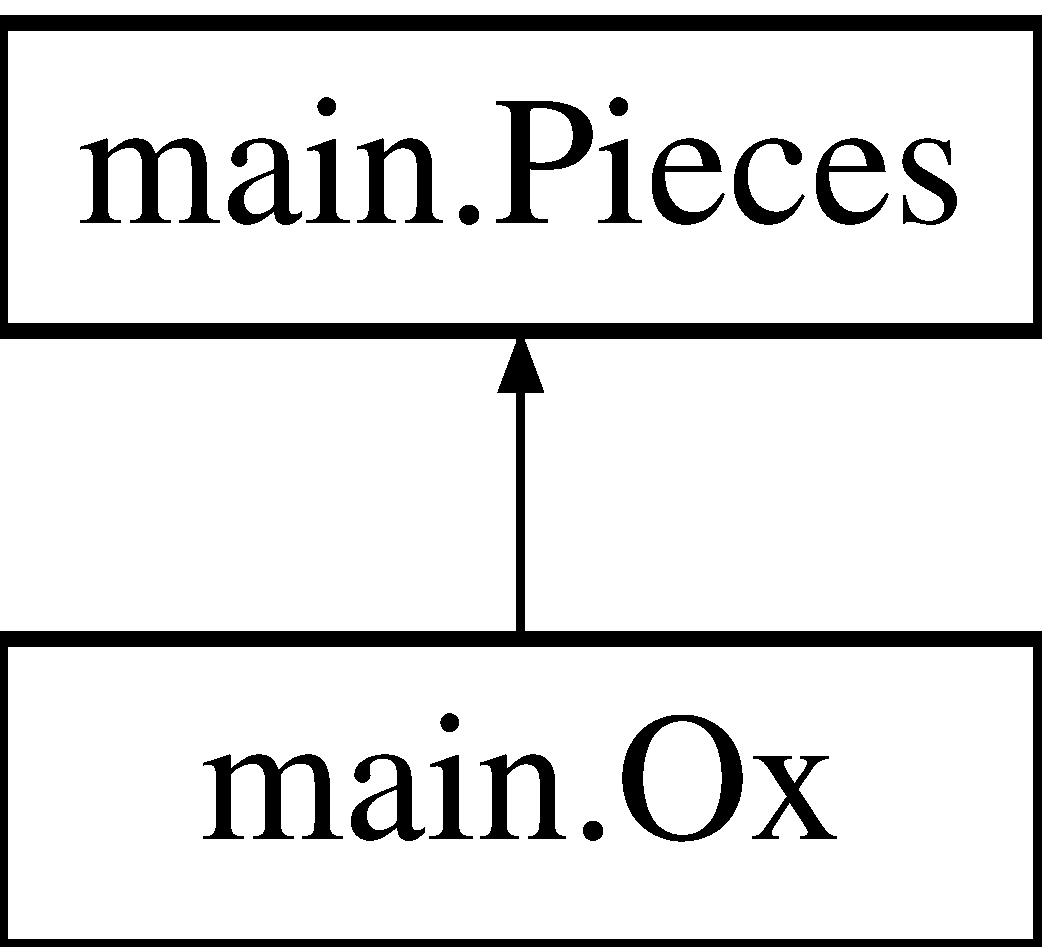
\includegraphics[height=2.000000cm]{classmain_1_1_ox}
\end{center}
\end{figure}
\subsection*{Public Member Functions}
\begin{DoxyCompactItemize}
\item 
\mbox{\hyperlink{classmain_1_1_ox_a1c423374c91b4af6701379f626507147}{Ox}} (int x, int y, int player)
\item 
boolean \mbox{\hyperlink{classmain_1_1_ox_aedafaea098b12d2a492cd2699510c62e}{is\+Valid\+Move}} (int newX, int newY)
\item 
boolean \mbox{\hyperlink{classmain_1_1_ox_a3963f0e93e390fe6a509a6a4da42f975}{valid\+Move}} (int newX, int newY, \mbox{\hyperlink{classmain_1_1_board}{Board}} board)
\item 
boolean \mbox{\hyperlink{classmain_1_1_ox_a73722f234f1025002c7d3a6c3613d126}{could\+Be\+Stopped}} (int newX, int newY, \mbox{\hyperlink{classmain_1_1_board}{Board}} board)
\item 
boolean \mbox{\hyperlink{classmain_1_1_ox_a29651061f20b6ca13c8a351e6121159f}{is\+Movable}} (\mbox{\hyperlink{classmain_1_1_board}{Board}} board)
\end{DoxyCompactItemize}
\subsection*{Additional Inherited Members}


\subsection{Detailed Description}
\begin{DoxyAuthor}{Author}
kaichenle 
\end{DoxyAuthor}


\subsection{Constructor \& Destructor Documentation}
\mbox{\Hypertarget{classmain_1_1_ox_a1c423374c91b4af6701379f626507147}\label{classmain_1_1_ox_a1c423374c91b4af6701379f626507147}} 
\index{main\+::\+Ox@{main\+::\+Ox}!Ox@{Ox}}
\index{Ox@{Ox}!main\+::\+Ox@{main\+::\+Ox}}
\subsubsection{\texorpdfstring{Ox()}{Ox()}}
{\footnotesize\ttfamily main.\+Ox.\+Ox (\begin{DoxyParamCaption}\item[{int}]{x,  }\item[{int}]{y,  }\item[{int}]{player }\end{DoxyParamCaption})\hspace{0.3cm}{\ttfamily [inline]}}

constructor 
\begin{DoxyParams}{Parameters}
{\em x} & x\+Coord \\
\hline
{\em y} & y\+Coord \\
\hline
{\em player} & player 1 or 2 \\
\hline
\end{DoxyParams}


\subsection{Member Function Documentation}
\mbox{\Hypertarget{classmain_1_1_ox_a73722f234f1025002c7d3a6c3613d126}\label{classmain_1_1_ox_a73722f234f1025002c7d3a6c3613d126}} 
\index{main\+::\+Ox@{main\+::\+Ox}!could\+Be\+Stopped@{could\+Be\+Stopped}}
\index{could\+Be\+Stopped@{could\+Be\+Stopped}!main\+::\+Ox@{main\+::\+Ox}}
\subsubsection{\texorpdfstring{could\+Be\+Stopped()}{couldBeStopped()}}
{\footnotesize\ttfamily boolean main.\+Ox.\+could\+Be\+Stopped (\begin{DoxyParamCaption}\item[{int}]{newX,  }\item[{int}]{newY,  }\item[{\mbox{\hyperlink{classmain_1_1_board}{Board}}}]{board }\end{DoxyParamCaption})\hspace{0.3cm}{\ttfamily [inline]}}

if any pieces could stop input \mbox{\hyperlink{classmain_1_1_ox}{Ox}} piece from x,y to newX newY 
\begin{DoxyParams}{Parameters}
{\em newX} & end x\+Coord \\
\hline
{\em newY} & end y\+Coord \\
\hline
{\em board} & that the chess play on \\
\hline
\end{DoxyParams}
\begin{DoxyReturn}{Returns}
true if there is a piece exists that can stop the chess otherwise false 
\end{DoxyReturn}
\mbox{\Hypertarget{classmain_1_1_ox_a29651061f20b6ca13c8a351e6121159f}\label{classmain_1_1_ox_a29651061f20b6ca13c8a351e6121159f}} 
\index{main\+::\+Ox@{main\+::\+Ox}!is\+Movable@{is\+Movable}}
\index{is\+Movable@{is\+Movable}!main\+::\+Ox@{main\+::\+Ox}}
\subsubsection{\texorpdfstring{is\+Movable()}{isMovable()}}
{\footnotesize\ttfamily boolean main.\+Ox.\+is\+Movable (\begin{DoxyParamCaption}\item[{\mbox{\hyperlink{classmain_1_1_board}{Board}}}]{board }\end{DoxyParamCaption})\hspace{0.3cm}{\ttfamily [inline]}}

helper functions check movability of \mbox{\hyperlink{classmain_1_1_ox}{Ox}} 
\begin{DoxyParams}{Parameters}
{\em board} & the game will be on \\
\hline
\end{DoxyParams}
\begin{DoxyReturn}{Returns}
true if the input can move otherwise false 
\end{DoxyReturn}
\mbox{\Hypertarget{classmain_1_1_ox_aedafaea098b12d2a492cd2699510c62e}\label{classmain_1_1_ox_aedafaea098b12d2a492cd2699510c62e}} 
\index{main\+::\+Ox@{main\+::\+Ox}!is\+Valid\+Move@{is\+Valid\+Move}}
\index{is\+Valid\+Move@{is\+Valid\+Move}!main\+::\+Ox@{main\+::\+Ox}}
\subsubsection{\texorpdfstring{is\+Valid\+Move()}{isValidMove()}}
{\footnotesize\ttfamily boolean main.\+Ox.\+is\+Valid\+Move (\begin{DoxyParamCaption}\item[{int}]{newX,  }\item[{int}]{newY }\end{DoxyParamCaption})\hspace{0.3cm}{\ttfamily [inline]}}

see if the chess move against convention without consider other chesses \mbox{\Hypertarget{classmain_1_1_ox_a3963f0e93e390fe6a509a6a4da42f975}\label{classmain_1_1_ox_a3963f0e93e390fe6a509a6a4da42f975}} 
\index{main\+::\+Ox@{main\+::\+Ox}!valid\+Move@{valid\+Move}}
\index{valid\+Move@{valid\+Move}!main\+::\+Ox@{main\+::\+Ox}}
\subsubsection{\texorpdfstring{valid\+Move()}{validMove()}}
{\footnotesize\ttfamily boolean main.\+Ox.\+valid\+Move (\begin{DoxyParamCaption}\item[{int}]{newX,  }\item[{int}]{newY,  }\item[{\mbox{\hyperlink{classmain_1_1_board}{Board}}}]{board }\end{DoxyParamCaption})\hspace{0.3cm}{\ttfamily [inline]}}

Helper functions check if it is a valid path to move \mbox{\hyperlink{classmain_1_1_ox}{Ox}}. It will be called inside move\+Chess with is\+Valid\+Move in each pieces subclass. This will check if there are pieces on the board that will influence the fact if it is valid to move chess 
\begin{DoxyParams}{Parameters}
{\em newX} & end y\+Coord \\
\hline
{\em newY} & end y\+Coord \\
\hline
{\em board} & the chess play on \\
\hline
\end{DoxyParams}
\begin{DoxyReturn}{Returns}
true if valid otherwise false 
\end{DoxyReturn}


The documentation for this class was generated from the following file\+:\begin{DoxyCompactItemize}
\item 
main/Ox.\+java\end{DoxyCompactItemize}

\hypertarget{classtests_1_1_ox_tests}{}\section{tests.\+Ox\+Tests Class Reference}
\label{classtests_1_1_ox_tests}\index{tests.\+Ox\+Tests@{tests.\+Ox\+Tests}}
\subsection*{Public Member Functions}
\begin{DoxyCompactItemize}
\item 
void \mbox{\hyperlink{classtests_1_1_ox_tests_a240476c2b7dda99ff721574bc2298fc9}{move\+Chess\+Ox}} ()
\item 
void \mbox{\hyperlink{classtests_1_1_ox_tests_a4567fa10ba9a7ecd39a334f80351155b}{is\+Movable\+Ox}} ()
\item 
void \mbox{\hyperlink{classtests_1_1_ox_tests_a67ebfc2f27b464501f96393654d2bbe8}{could\+Be\+Stopped\+Ox}} ()
\end{DoxyCompactItemize}


\subsection{Member Function Documentation}
\mbox{\Hypertarget{classtests_1_1_ox_tests_a67ebfc2f27b464501f96393654d2bbe8}\label{classtests_1_1_ox_tests_a67ebfc2f27b464501f96393654d2bbe8}} 
\index{tests\+::\+Ox\+Tests@{tests\+::\+Ox\+Tests}!could\+Be\+Stopped\+Ox@{could\+Be\+Stopped\+Ox}}
\index{could\+Be\+Stopped\+Ox@{could\+Be\+Stopped\+Ox}!tests\+::\+Ox\+Tests@{tests\+::\+Ox\+Tests}}
\subsubsection{\texorpdfstring{could\+Be\+Stopped\+Ox()}{couldBeStoppedOx()}}
{\footnotesize\ttfamily void tests.\+Ox\+Tests.\+could\+Be\+Stopped\+Ox (\begin{DoxyParamCaption}{ }\end{DoxyParamCaption})\hspace{0.3cm}{\ttfamily [inline]}}

test on could\+Be\+Stopped \mbox{\Hypertarget{classtests_1_1_ox_tests_a4567fa10ba9a7ecd39a334f80351155b}\label{classtests_1_1_ox_tests_a4567fa10ba9a7ecd39a334f80351155b}} 
\index{tests\+::\+Ox\+Tests@{tests\+::\+Ox\+Tests}!is\+Movable\+Ox@{is\+Movable\+Ox}}
\index{is\+Movable\+Ox@{is\+Movable\+Ox}!tests\+::\+Ox\+Tests@{tests\+::\+Ox\+Tests}}
\subsubsection{\texorpdfstring{is\+Movable\+Ox()}{isMovableOx()}}
{\footnotesize\ttfamily void tests.\+Ox\+Tests.\+is\+Movable\+Ox (\begin{DoxyParamCaption}{ }\end{DoxyParamCaption})\hspace{0.3cm}{\ttfamily [inline]}}

test on is\+Movable \mbox{\Hypertarget{classtests_1_1_ox_tests_a240476c2b7dda99ff721574bc2298fc9}\label{classtests_1_1_ox_tests_a240476c2b7dda99ff721574bc2298fc9}} 
\index{tests\+::\+Ox\+Tests@{tests\+::\+Ox\+Tests}!move\+Chess\+Ox@{move\+Chess\+Ox}}
\index{move\+Chess\+Ox@{move\+Chess\+Ox}!tests\+::\+Ox\+Tests@{tests\+::\+Ox\+Tests}}
\subsubsection{\texorpdfstring{move\+Chess\+Ox()}{moveChessOx()}}
{\footnotesize\ttfamily void tests.\+Ox\+Tests.\+move\+Chess\+Ox (\begin{DoxyParamCaption}{ }\end{DoxyParamCaption})\hspace{0.3cm}{\ttfamily [inline]}}

test on move\+Chess 

The documentation for this class was generated from the following file\+:\begin{DoxyCompactItemize}
\item 
tests/Ox\+Tests.\+java\end{DoxyCompactItemize}

\hypertarget{classmain_1_1_pawn}{}\section{main.\+Pawn Class Reference}
\label{classmain_1_1_pawn}\index{main.\+Pawn@{main.\+Pawn}}
Inheritance diagram for main.\+Pawn\+:\begin{figure}[H]
\begin{center}
\leavevmode
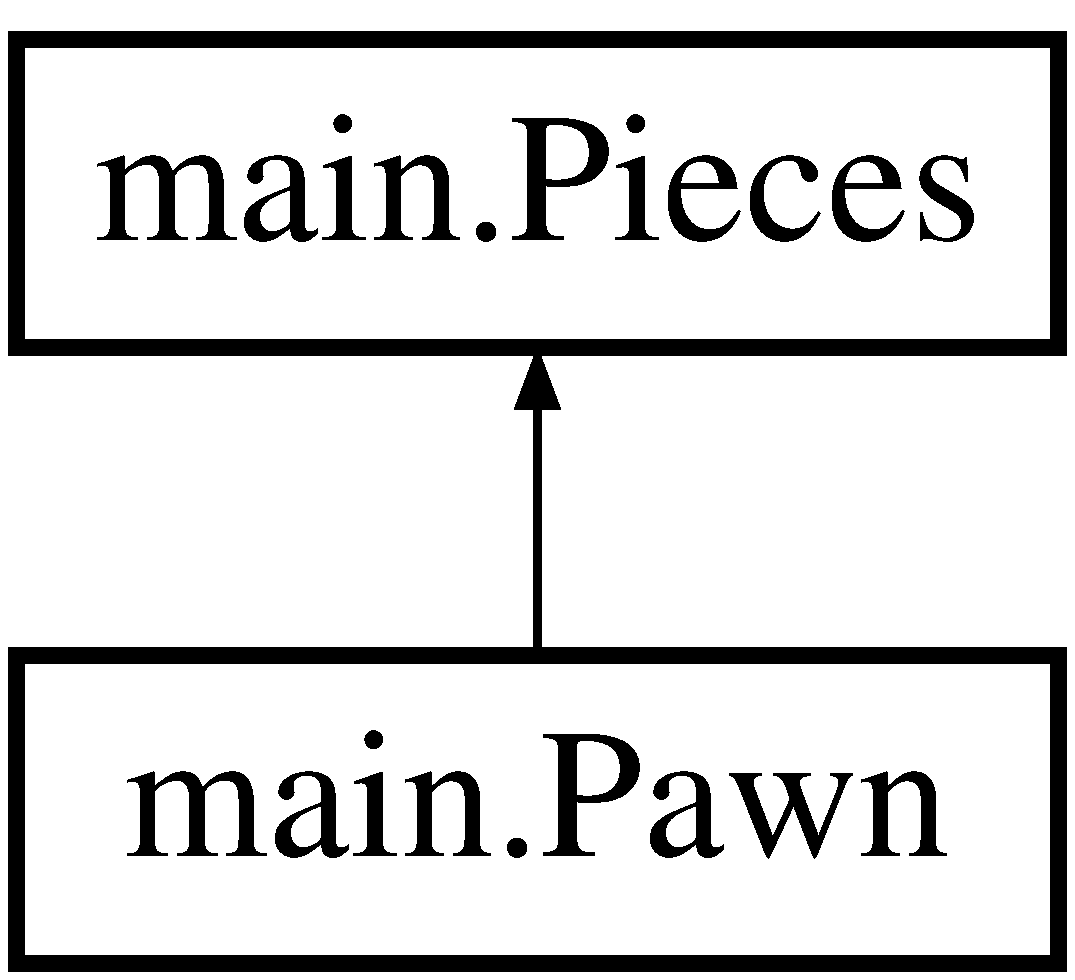
\includegraphics[height=2.000000cm]{classmain_1_1_pawn}
\end{center}
\end{figure}
\subsection*{Public Member Functions}
\begin{DoxyCompactItemize}
\item 
\mbox{\hyperlink{classmain_1_1_pawn_ad6b3f84806779b0a498cccc9118b1978}{Pawn}} (int x, int y, int player)
\item 
boolean \mbox{\hyperlink{classmain_1_1_pawn_ac7b5fb5e1e8d062f479483e4c506b158}{is\+Valid\+Move}} (int newX, int newY)
\item 
boolean \mbox{\hyperlink{classmain_1_1_pawn_abf4a219aa514708a23dcf6999bf1e1e7}{valid\+Move}} (int newX, int newY, \mbox{\hyperlink{classmain_1_1_board}{Board}} board)
\item 
boolean \mbox{\hyperlink{classmain_1_1_pawn_a117c6ed884c1233e27f2a5c5f1ea379c}{could\+Be\+Stopped}} (int newX, int newY, \mbox{\hyperlink{classmain_1_1_board}{Board}} board)
\item 
boolean \mbox{\hyperlink{classmain_1_1_pawn_a54608094adc31c72a7ab0ff192a54f4d}{is\+Movable}} (\mbox{\hyperlink{classmain_1_1_board}{Board}} board)
\end{DoxyCompactItemize}
\subsection*{Additional Inherited Members}


\subsection{Detailed Description}
\begin{DoxyAuthor}{Author}
kaichenle 
\end{DoxyAuthor}


\subsection{Constructor \& Destructor Documentation}
\mbox{\Hypertarget{classmain_1_1_pawn_ad6b3f84806779b0a498cccc9118b1978}\label{classmain_1_1_pawn_ad6b3f84806779b0a498cccc9118b1978}} 
\index{main\+::\+Pawn@{main\+::\+Pawn}!Pawn@{Pawn}}
\index{Pawn@{Pawn}!main\+::\+Pawn@{main\+::\+Pawn}}
\subsubsection{\texorpdfstring{Pawn()}{Pawn()}}
{\footnotesize\ttfamily main.\+Pawn.\+Pawn (\begin{DoxyParamCaption}\item[{int}]{x,  }\item[{int}]{y,  }\item[{int}]{player }\end{DoxyParamCaption})\hspace{0.3cm}{\ttfamily [inline]}}

constructor 
\begin{DoxyParams}{Parameters}
{\em x} & x\+Coord \\
\hline
{\em y} & y\+Coord \\
\hline
{\em player} & player 1 or 2 \\
\hline
\end{DoxyParams}


\subsection{Member Function Documentation}
\mbox{\Hypertarget{classmain_1_1_pawn_a117c6ed884c1233e27f2a5c5f1ea379c}\label{classmain_1_1_pawn_a117c6ed884c1233e27f2a5c5f1ea379c}} 
\index{main\+::\+Pawn@{main\+::\+Pawn}!could\+Be\+Stopped@{could\+Be\+Stopped}}
\index{could\+Be\+Stopped@{could\+Be\+Stopped}!main\+::\+Pawn@{main\+::\+Pawn}}
\subsubsection{\texorpdfstring{could\+Be\+Stopped()}{couldBeStopped()}}
{\footnotesize\ttfamily boolean main.\+Pawn.\+could\+Be\+Stopped (\begin{DoxyParamCaption}\item[{int}]{newX,  }\item[{int}]{newY,  }\item[{\mbox{\hyperlink{classmain_1_1_board}{Board}}}]{board }\end{DoxyParamCaption})\hspace{0.3cm}{\ttfamily [inline]}}

if any pieces could stop input bishop or queen(diaganol) piece from x,y to newX newY 
\begin{DoxyParams}{Parameters}
{\em newX} & end x\+Coord \\
\hline
{\em newY} & end y\+Coord \\
\hline
{\em board} & the game will play on \\
\hline
\end{DoxyParams}
\begin{DoxyReturn}{Returns}
true if there is a piece exists otherwise false 
\end{DoxyReturn}
\mbox{\Hypertarget{classmain_1_1_pawn_a54608094adc31c72a7ab0ff192a54f4d}\label{classmain_1_1_pawn_a54608094adc31c72a7ab0ff192a54f4d}} 
\index{main\+::\+Pawn@{main\+::\+Pawn}!is\+Movable@{is\+Movable}}
\index{is\+Movable@{is\+Movable}!main\+::\+Pawn@{main\+::\+Pawn}}
\subsubsection{\texorpdfstring{is\+Movable()}{isMovable()}}
{\footnotesize\ttfamily boolean main.\+Pawn.\+is\+Movable (\begin{DoxyParamCaption}\item[{\mbox{\hyperlink{classmain_1_1_board}{Board}}}]{board }\end{DoxyParamCaption})\hspace{0.3cm}{\ttfamily [inline]}}

helper functions check movability of pawn 
\begin{DoxyParams}{Parameters}
{\em board} & the game will be on \\
\hline
\end{DoxyParams}
\begin{DoxyReturn}{Returns}
true if the input can move otherwise false 
\end{DoxyReturn}
\mbox{\Hypertarget{classmain_1_1_pawn_ac7b5fb5e1e8d062f479483e4c506b158}\label{classmain_1_1_pawn_ac7b5fb5e1e8d062f479483e4c506b158}} 
\index{main\+::\+Pawn@{main\+::\+Pawn}!is\+Valid\+Move@{is\+Valid\+Move}}
\index{is\+Valid\+Move@{is\+Valid\+Move}!main\+::\+Pawn@{main\+::\+Pawn}}
\subsubsection{\texorpdfstring{is\+Valid\+Move()}{isValidMove()}}
{\footnotesize\ttfamily boolean main.\+Pawn.\+is\+Valid\+Move (\begin{DoxyParamCaption}\item[{int}]{newX,  }\item[{int}]{newY }\end{DoxyParamCaption})\hspace{0.3cm}{\ttfamily [inline]}}

see if the chess move against convention without consider other chesses \mbox{\Hypertarget{classmain_1_1_pawn_abf4a219aa514708a23dcf6999bf1e1e7}\label{classmain_1_1_pawn_abf4a219aa514708a23dcf6999bf1e1e7}} 
\index{main\+::\+Pawn@{main\+::\+Pawn}!valid\+Move@{valid\+Move}}
\index{valid\+Move@{valid\+Move}!main\+::\+Pawn@{main\+::\+Pawn}}
\subsubsection{\texorpdfstring{valid\+Move()}{validMove()}}
{\footnotesize\ttfamily boolean main.\+Pawn.\+valid\+Move (\begin{DoxyParamCaption}\item[{int}]{newX,  }\item[{int}]{newY,  }\item[{\mbox{\hyperlink{classmain_1_1_board}{Board}}}]{board }\end{DoxyParamCaption})\hspace{0.3cm}{\ttfamily [inline]}}

Helper functions check if it is a valid path to move \mbox{\hyperlink{classmain_1_1_pawn}{Pawn}}. It will be called inside move\+Chess with is\+Valid\+Move in each pieces subclass. This will check if there are pieces on the board that will influence the fact if it is valid to move chess 
\begin{DoxyParams}{Parameters}
{\em newX} & end y\+Coord \\
\hline
{\em newY} & end y\+Coord \\
\hline
{\em board} & the chess will play on \\
\hline
\end{DoxyParams}
\begin{DoxyReturn}{Returns}
true if valid otherwise false 
\end{DoxyReturn}


The documentation for this class was generated from the following file\+:\begin{DoxyCompactItemize}
\item 
main/Pawn.\+java\end{DoxyCompactItemize}

\hypertarget{classtests_1_1_pawn_tests}{}\section{tests.\+Pawn\+Tests Class Reference}
\label{classtests_1_1_pawn_tests}\index{tests.\+Pawn\+Tests@{tests.\+Pawn\+Tests}}
\subsection*{Public Member Functions}
\begin{DoxyCompactItemize}
\item 
void \mbox{\hyperlink{classtests_1_1_pawn_tests_aec235d730a400fc8ad186a7ee14680fd}{should\+Move\+Pawn}} ()
\end{DoxyCompactItemize}


\subsection{Detailed Description}
\begin{DoxyAuthor}{Author}
kaichenle 
\end{DoxyAuthor}


\subsection{Member Function Documentation}
\mbox{\Hypertarget{classtests_1_1_pawn_tests_aec235d730a400fc8ad186a7ee14680fd}\label{classtests_1_1_pawn_tests_aec235d730a400fc8ad186a7ee14680fd}} 
\index{tests\+::\+Pawn\+Tests@{tests\+::\+Pawn\+Tests}!should\+Move\+Pawn@{should\+Move\+Pawn}}
\index{should\+Move\+Pawn@{should\+Move\+Pawn}!tests\+::\+Pawn\+Tests@{tests\+::\+Pawn\+Tests}}
\subsubsection{\texorpdfstring{should\+Move\+Pawn()}{shouldMovePawn()}}
{\footnotesize\ttfamily void tests.\+Pawn\+Tests.\+should\+Move\+Pawn (\begin{DoxyParamCaption}{ }\end{DoxyParamCaption})\hspace{0.3cm}{\ttfamily [inline]}}

test on move\+Chess 

The documentation for this class was generated from the following file\+:\begin{DoxyCompactItemize}
\item 
tests/Pawn\+Tests.\+java\end{DoxyCompactItemize}

\hypertarget{classmain_1_1_pieces}{}\section{main.\+Pieces Class Reference}
\label{classmain_1_1_pieces}\index{main.\+Pieces@{main.\+Pieces}}
Inheritance diagram for main.\+Pieces\+:\begin{figure}[H]
\begin{center}
\leavevmode
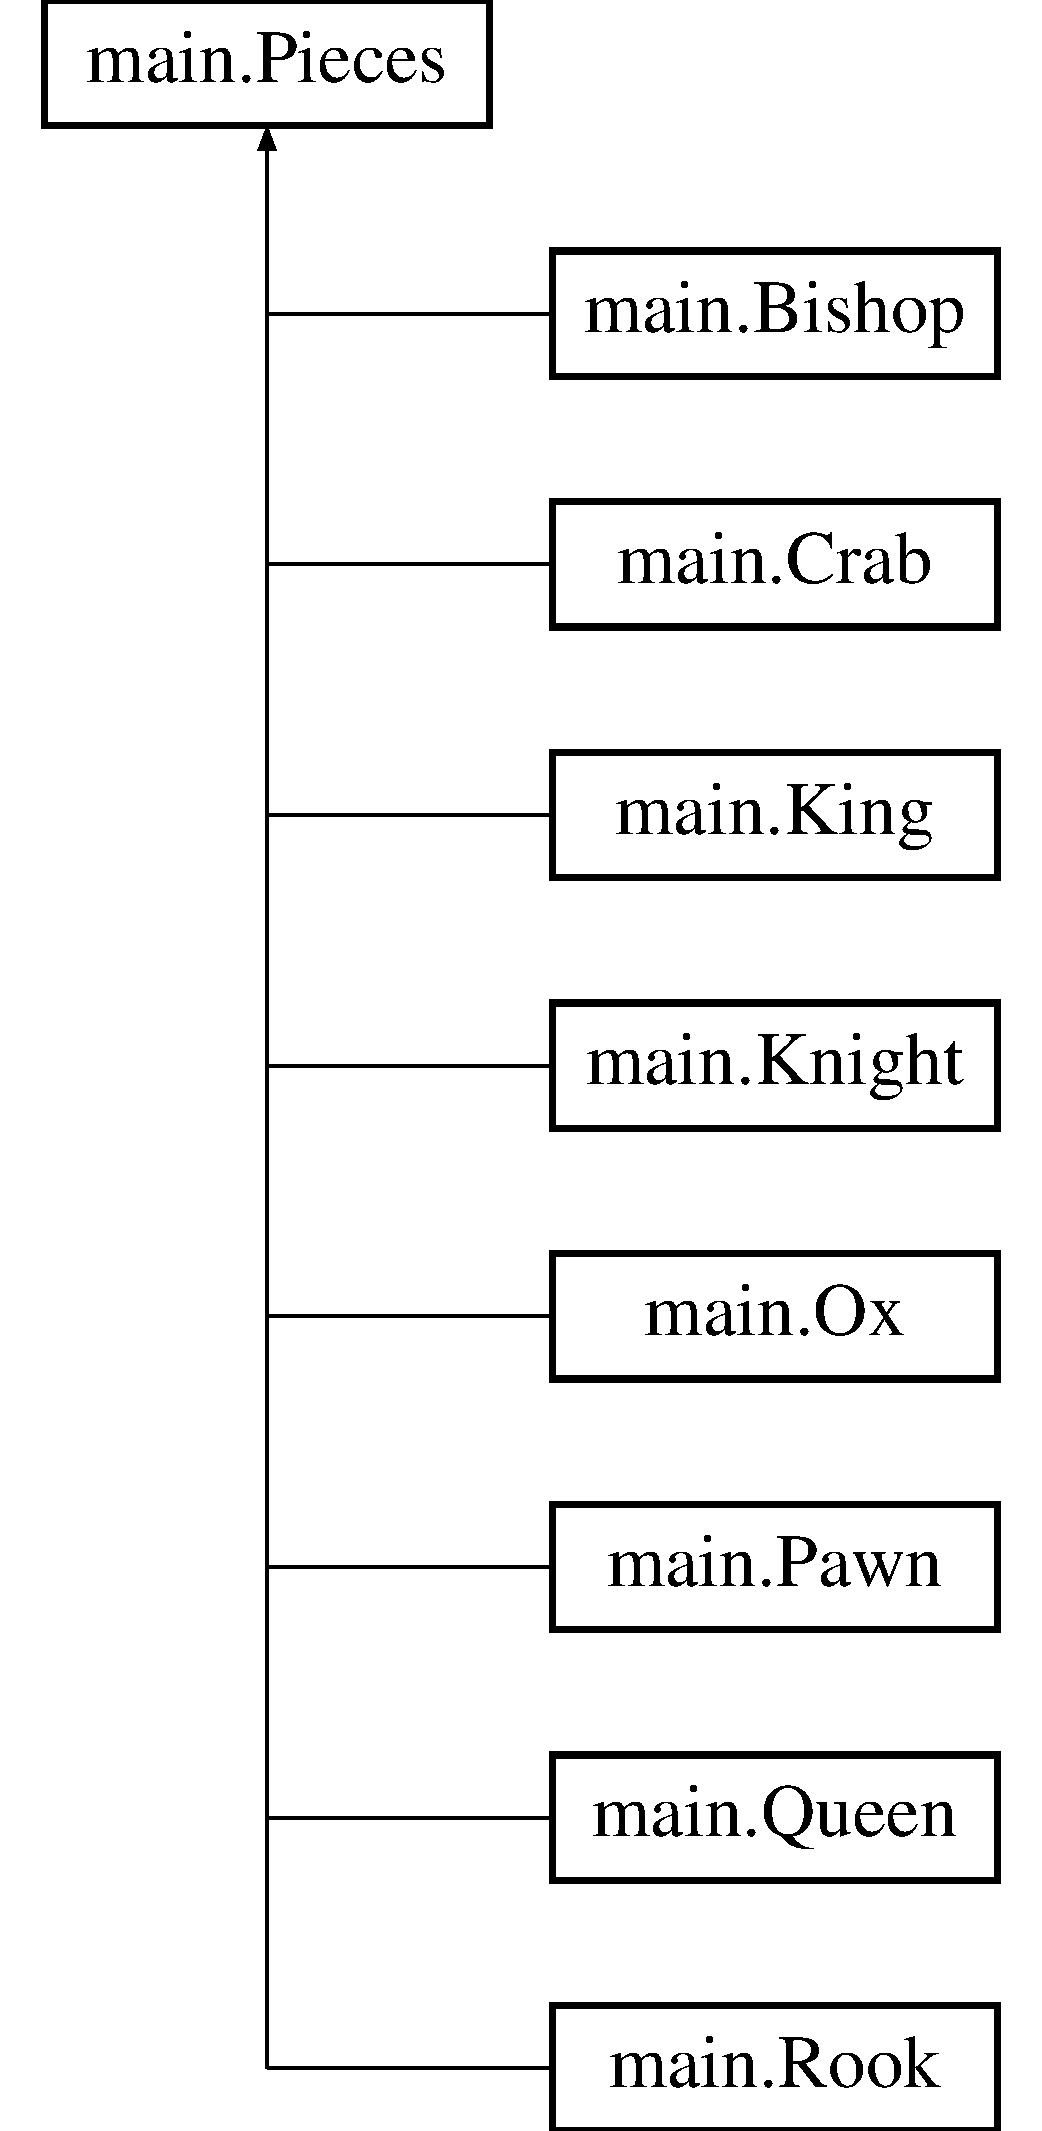
\includegraphics[height=9.000000cm]{classmain_1_1_pieces}
\end{center}
\end{figure}
\subsection*{Public Member Functions}
\begin{DoxyCompactItemize}
\item 
\mbox{\hyperlink{classmain_1_1_pieces_aa626e806bdd56045f481edb81dc217dd}{Pieces}} (int x, int y, int player)
\item 
boolean \mbox{\hyperlink{classmain_1_1_pieces_a02d805a58894aca8a12be4dce0ae4125}{out\+Of\+Boundry\+Or\+Not\+Move}} (int x, int y)
\item 
abstract boolean \mbox{\hyperlink{classmain_1_1_pieces_ab9e56890f37271b7eddadd7b634157b1}{is\+Valid\+Move}} (int newX, int newY)
\item 
\mbox{\Hypertarget{classmain_1_1_pieces_ab77cb1de1e9c3f171a69655c3bf7514c}\label{classmain_1_1_pieces_ab77cb1de1e9c3f171a69655c3bf7514c}} 
abstract boolean {\bfseries valid\+Move} (int newX, int newY, \mbox{\hyperlink{classmain_1_1_board}{Board}} board)
\item 
\mbox{\Hypertarget{classmain_1_1_pieces_a96608930fc453fe197d0f4cb006823ed}\label{classmain_1_1_pieces_a96608930fc453fe197d0f4cb006823ed}} 
abstract boolean {\bfseries could\+Be\+Stopped} (int newX, int newY, \mbox{\hyperlink{classmain_1_1_board}{Board}} board)
\item 
\mbox{\Hypertarget{classmain_1_1_pieces_a6b3abc04fc214b01781662e4533b2b6f}\label{classmain_1_1_pieces_a6b3abc04fc214b01781662e4533b2b6f}} 
abstract boolean {\bfseries is\+Movable} (\mbox{\hyperlink{classmain_1_1_board}{Board}} board)
\end{DoxyCompactItemize}
\subsection*{Public Attributes}
\begin{DoxyCompactItemize}
\item 
\mbox{\Hypertarget{classmain_1_1_pieces_ab7c9b25dca64d565c9660381f35a7d1b}\label{classmain_1_1_pieces_ab7c9b25dca64d565c9660381f35a7d1b}} 
int {\bfseries x} = -\/1
\item 
\mbox{\Hypertarget{classmain_1_1_pieces_a8da9a1ccb36051e345943c7f20d257f3}\label{classmain_1_1_pieces_a8da9a1ccb36051e345943c7f20d257f3}} 
int {\bfseries y} = -\/1
\item 
\mbox{\Hypertarget{classmain_1_1_pieces_a04cbc94744f8532a295e2bf0201e18fa}\label{classmain_1_1_pieces_a04cbc94744f8532a295e2bf0201e18fa}} 
int {\bfseries player} = -\/1
\item 
\mbox{\Hypertarget{classmain_1_1_pieces_a80df8799af3282b704681e9c1b3eb37f}\label{classmain_1_1_pieces_a80df8799af3282b704681e9c1b3eb37f}} 
String {\bfseries type} = \char`\"{}\char`\"{}
\end{DoxyCompactItemize}


\subsection{Detailed Description}
\mbox{\hyperlink{classmain_1_1_pieces}{Pieces}} is a parent class. \mbox{\hyperlink{classmain_1_1_king}{King}}, \mbox{\hyperlink{classmain_1_1_pawn}{Pawn}}, \mbox{\hyperlink{classmain_1_1_queen}{Queen}} etc. are different kind of chesses(subclass) \begin{DoxyAuthor}{Author}
kaichenle 
\end{DoxyAuthor}


\subsection{Constructor \& Destructor Documentation}
\mbox{\Hypertarget{classmain_1_1_pieces_aa626e806bdd56045f481edb81dc217dd}\label{classmain_1_1_pieces_aa626e806bdd56045f481edb81dc217dd}} 
\index{main\+::\+Pieces@{main\+::\+Pieces}!Pieces@{Pieces}}
\index{Pieces@{Pieces}!main\+::\+Pieces@{main\+::\+Pieces}}
\subsubsection{\texorpdfstring{Pieces()}{Pieces()}}
{\footnotesize\ttfamily main.\+Pieces.\+Pieces (\begin{DoxyParamCaption}\item[{int}]{x,  }\item[{int}]{y,  }\item[{int}]{player }\end{DoxyParamCaption})\hspace{0.3cm}{\ttfamily [inline]}}

Constructor of the super class 
\begin{DoxyParams}{Parameters}
{\em x} & \\
\hline
{\em y} & \\
\hline
{\em player} & \\
\hline
\end{DoxyParams}


\subsection{Member Function Documentation}
\mbox{\Hypertarget{classmain_1_1_pieces_ab9e56890f37271b7eddadd7b634157b1}\label{classmain_1_1_pieces_ab9e56890f37271b7eddadd7b634157b1}} 
\index{main\+::\+Pieces@{main\+::\+Pieces}!is\+Valid\+Move@{is\+Valid\+Move}}
\index{is\+Valid\+Move@{is\+Valid\+Move}!main\+::\+Pieces@{main\+::\+Pieces}}
\subsubsection{\texorpdfstring{is\+Valid\+Move()}{isValidMove()}}
{\footnotesize\ttfamily abstract boolean main.\+Pieces.\+is\+Valid\+Move (\begin{DoxyParamCaption}\item[{int}]{newX,  }\item[{int}]{newY }\end{DoxyParamCaption})\hspace{0.3cm}{\ttfamily [abstract]}}

abstract function implemented in each subclass that check if it is valid for the pieces to move (without consider the other pieces) 
\begin{DoxyParams}{Parameters}
{\em newX} & x Coord \\
\hline
{\em newY} & y Coord \\
\hline
\end{DoxyParams}
\begin{DoxyReturn}{Returns}
true when it is valid to move by convention 
\end{DoxyReturn}
\mbox{\Hypertarget{classmain_1_1_pieces_a02d805a58894aca8a12be4dce0ae4125}\label{classmain_1_1_pieces_a02d805a58894aca8a12be4dce0ae4125}} 
\index{main\+::\+Pieces@{main\+::\+Pieces}!out\+Of\+Boundry\+Or\+Not\+Move@{out\+Of\+Boundry\+Or\+Not\+Move}}
\index{out\+Of\+Boundry\+Or\+Not\+Move@{out\+Of\+Boundry\+Or\+Not\+Move}!main\+::\+Pieces@{main\+::\+Pieces}}
\subsubsection{\texorpdfstring{out\+Of\+Boundry\+Or\+Not\+Move()}{outOfBoundryOrNotMove()}}
{\footnotesize\ttfamily boolean main.\+Pieces.\+out\+Of\+Boundry\+Or\+Not\+Move (\begin{DoxyParamCaption}\item[{int}]{x,  }\item[{int}]{y }\end{DoxyParamCaption})\hspace{0.3cm}{\ttfamily [inline]}}

a helper function check if the chess try to move out of bound or not move 
\begin{DoxyParams}{Parameters}
{\em x} & \\
\hline
{\em y} & \\
\hline
\end{DoxyParams}
\begin{DoxyReturn}{Returns}
return true if it is not out of boundry and actually change x or y or both return false otherwise 
\end{DoxyReturn}


The documentation for this class was generated from the following file\+:\begin{DoxyCompactItemize}
\item 
main/Pieces.\+java\end{DoxyCompactItemize}

\hypertarget{classmain_1_1_queen}{}\section{main.\+Queen Class Reference}
\label{classmain_1_1_queen}\index{main.\+Queen@{main.\+Queen}}
Inheritance diagram for main.\+Queen\+:\begin{figure}[H]
\begin{center}
\leavevmode
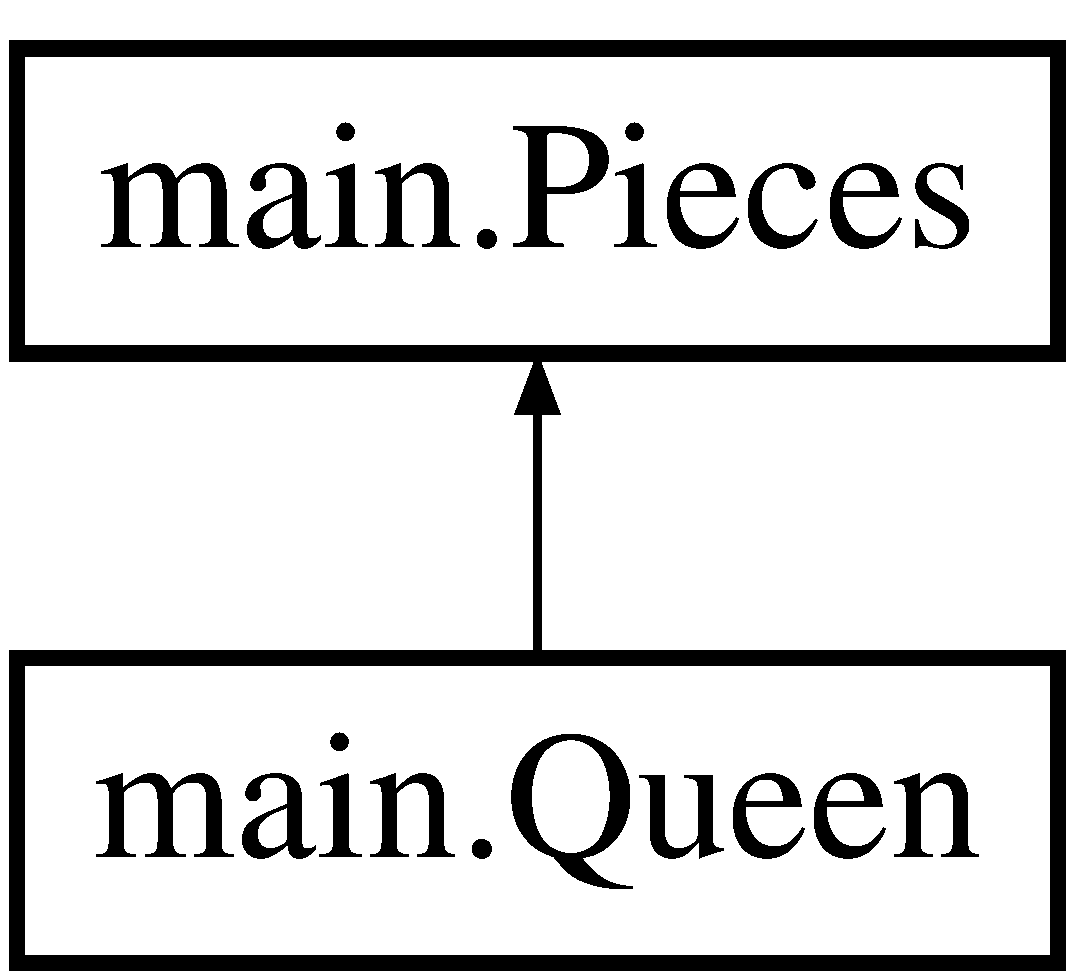
\includegraphics[height=2.000000cm]{classmain_1_1_queen}
\end{center}
\end{figure}
\subsection*{Public Member Functions}
\begin{DoxyCompactItemize}
\item 
\mbox{\hyperlink{classmain_1_1_queen_ac10f8437486c3ef5ed097034131aba57}{Queen}} (int x, int y, int player)
\item 
boolean \mbox{\hyperlink{classmain_1_1_queen_a0081a5d2f2b4c5e4424dc0db0cff7c4e}{is\+Valid\+Move}} (int newX, int newY)
\item 
boolean \mbox{\hyperlink{classmain_1_1_queen_a47c07514768b4d9cb4b1e60a5bd61fd7}{valid\+Move}} (int newX, int newY, \mbox{\hyperlink{classmain_1_1_board}{Board}} board)
\item 
boolean \mbox{\hyperlink{classmain_1_1_queen_ac4a78f8305a5ce34f14a77691905af79}{could\+Be\+Stopped}} (int newX, int newY, \mbox{\hyperlink{classmain_1_1_board}{Board}} board)
\item 
boolean \mbox{\hyperlink{classmain_1_1_queen_aefc0bc7f1a1603ce266d54cd9cc16676}{is\+Movable}} (\mbox{\hyperlink{classmain_1_1_board}{Board}} board)
\end{DoxyCompactItemize}
\subsection*{Additional Inherited Members}


\subsection{Detailed Description}
\begin{DoxyAuthor}{Author}
kaichenle 
\end{DoxyAuthor}


\subsection{Constructor \& Destructor Documentation}
\mbox{\Hypertarget{classmain_1_1_queen_ac10f8437486c3ef5ed097034131aba57}\label{classmain_1_1_queen_ac10f8437486c3ef5ed097034131aba57}} 
\index{main\+::\+Queen@{main\+::\+Queen}!Queen@{Queen}}
\index{Queen@{Queen}!main\+::\+Queen@{main\+::\+Queen}}
\subsubsection{\texorpdfstring{Queen()}{Queen()}}
{\footnotesize\ttfamily main.\+Queen.\+Queen (\begin{DoxyParamCaption}\item[{int}]{x,  }\item[{int}]{y,  }\item[{int}]{player }\end{DoxyParamCaption})\hspace{0.3cm}{\ttfamily [inline]}}

constructor 
\begin{DoxyParams}{Parameters}
{\em x} & x\+Coord \\
\hline
{\em y} & y\+Coord \\
\hline
{\em player} & player 1 or 2 \\
\hline
\end{DoxyParams}


\subsection{Member Function Documentation}
\mbox{\Hypertarget{classmain_1_1_queen_ac4a78f8305a5ce34f14a77691905af79}\label{classmain_1_1_queen_ac4a78f8305a5ce34f14a77691905af79}} 
\index{main\+::\+Queen@{main\+::\+Queen}!could\+Be\+Stopped@{could\+Be\+Stopped}}
\index{could\+Be\+Stopped@{could\+Be\+Stopped}!main\+::\+Queen@{main\+::\+Queen}}
\subsubsection{\texorpdfstring{could\+Be\+Stopped()}{couldBeStopped()}}
{\footnotesize\ttfamily boolean main.\+Queen.\+could\+Be\+Stopped (\begin{DoxyParamCaption}\item[{int}]{newX,  }\item[{int}]{newY,  }\item[{\mbox{\hyperlink{classmain_1_1_board}{Board}}}]{board }\end{DoxyParamCaption})\hspace{0.3cm}{\ttfamily [inline]}}

if any pieces could stop input bishop or queen(diaganol) piece from x,y to newX newY 
\begin{DoxyParams}{Parameters}
{\em newX} & end x\+Coord \\
\hline
{\em newY} & end y\+Coord \\
\hline
{\em board} & the game will play on \\
\hline
\end{DoxyParams}
\begin{DoxyReturn}{Returns}
true if there is a piece exists otherwise false 
\end{DoxyReturn}
\mbox{\Hypertarget{classmain_1_1_queen_aefc0bc7f1a1603ce266d54cd9cc16676}\label{classmain_1_1_queen_aefc0bc7f1a1603ce266d54cd9cc16676}} 
\index{main\+::\+Queen@{main\+::\+Queen}!is\+Movable@{is\+Movable}}
\index{is\+Movable@{is\+Movable}!main\+::\+Queen@{main\+::\+Queen}}
\subsubsection{\texorpdfstring{is\+Movable()}{isMovable()}}
{\footnotesize\ttfamily boolean main.\+Queen.\+is\+Movable (\begin{DoxyParamCaption}\item[{\mbox{\hyperlink{classmain_1_1_board}{Board}}}]{board }\end{DoxyParamCaption})\hspace{0.3cm}{\ttfamily [inline]}}

helper functions check movability of bishop or queen(diaganol) 
\begin{DoxyParams}{Parameters}
{\em board} & the game will be on \\
\hline
\end{DoxyParams}
\begin{DoxyReturn}{Returns}
true if the input can move otherwise false 
\end{DoxyReturn}
\mbox{\Hypertarget{classmain_1_1_queen_a0081a5d2f2b4c5e4424dc0db0cff7c4e}\label{classmain_1_1_queen_a0081a5d2f2b4c5e4424dc0db0cff7c4e}} 
\index{main\+::\+Queen@{main\+::\+Queen}!is\+Valid\+Move@{is\+Valid\+Move}}
\index{is\+Valid\+Move@{is\+Valid\+Move}!main\+::\+Queen@{main\+::\+Queen}}
\subsubsection{\texorpdfstring{is\+Valid\+Move()}{isValidMove()}}
{\footnotesize\ttfamily boolean main.\+Queen.\+is\+Valid\+Move (\begin{DoxyParamCaption}\item[{int}]{newX,  }\item[{int}]{newY }\end{DoxyParamCaption})\hspace{0.3cm}{\ttfamily [inline]}}

see if the chess move against convention without consider other chesses \mbox{\Hypertarget{classmain_1_1_queen_a47c07514768b4d9cb4b1e60a5bd61fd7}\label{classmain_1_1_queen_a47c07514768b4d9cb4b1e60a5bd61fd7}} 
\index{main\+::\+Queen@{main\+::\+Queen}!valid\+Move@{valid\+Move}}
\index{valid\+Move@{valid\+Move}!main\+::\+Queen@{main\+::\+Queen}}
\subsubsection{\texorpdfstring{valid\+Move()}{validMove()}}
{\footnotesize\ttfamily boolean main.\+Queen.\+valid\+Move (\begin{DoxyParamCaption}\item[{int}]{newX,  }\item[{int}]{newY,  }\item[{\mbox{\hyperlink{classmain_1_1_board}{Board}}}]{board }\end{DoxyParamCaption})\hspace{0.3cm}{\ttfamily [inline]}}

Helper functions check if it is a valid path to move \mbox{\hyperlink{classmain_1_1_queen}{Queen}}. It will be called inside move\+Chess with is\+Valid\+Move in each pieces subclass. This will check if there are pieces on the board that will influence the fact if it is valid to move chess 
\begin{DoxyParams}{Parameters}
{\em newX} & end y\+Coord \\
\hline
{\em newY} & end y\+Coord \\
\hline
{\em board} & the game will play on \\
\hline
\end{DoxyParams}
\begin{DoxyReturn}{Returns}
true if valid otherwise false 
\end{DoxyReturn}


The documentation for this class was generated from the following file\+:\begin{DoxyCompactItemize}
\item 
main/Queen.\+java\end{DoxyCompactItemize}

\hypertarget{classtests_1_1_queen_tests}{}\section{tests.\+Queen\+Tests Class Reference}
\label{classtests_1_1_queen_tests}\index{tests.\+Queen\+Tests@{tests.\+Queen\+Tests}}
\subsection*{Public Member Functions}
\begin{DoxyCompactItemize}
\item 
void \mbox{\hyperlink{classtests_1_1_queen_tests_a0b36ca704b99d0b5ff60e2a4556b0332}{should\+Move\+Queen}} ()
\end{DoxyCompactItemize}


\subsection{Detailed Description}
\begin{DoxyAuthor}{Author}
kaichenle 
\end{DoxyAuthor}


\subsection{Member Function Documentation}
\mbox{\Hypertarget{classtests_1_1_queen_tests_a0b36ca704b99d0b5ff60e2a4556b0332}\label{classtests_1_1_queen_tests_a0b36ca704b99d0b5ff60e2a4556b0332}} 
\index{tests\+::\+Queen\+Tests@{tests\+::\+Queen\+Tests}!should\+Move\+Queen@{should\+Move\+Queen}}
\index{should\+Move\+Queen@{should\+Move\+Queen}!tests\+::\+Queen\+Tests@{tests\+::\+Queen\+Tests}}
\subsubsection{\texorpdfstring{should\+Move\+Queen()}{shouldMoveQueen()}}
{\footnotesize\ttfamily void tests.\+Queen\+Tests.\+should\+Move\+Queen (\begin{DoxyParamCaption}{ }\end{DoxyParamCaption})\hspace{0.3cm}{\ttfamily [inline]}}

test on move\+Chess 

The documentation for this class was generated from the following file\+:\begin{DoxyCompactItemize}
\item 
tests/Queen\+Tests.\+java\end{DoxyCompactItemize}

\hypertarget{classmain_1_1_rook}{}\section{main.\+Rook Class Reference}
\label{classmain_1_1_rook}\index{main.\+Rook@{main.\+Rook}}
Inheritance diagram for main.\+Rook\+:\begin{figure}[H]
\begin{center}
\leavevmode
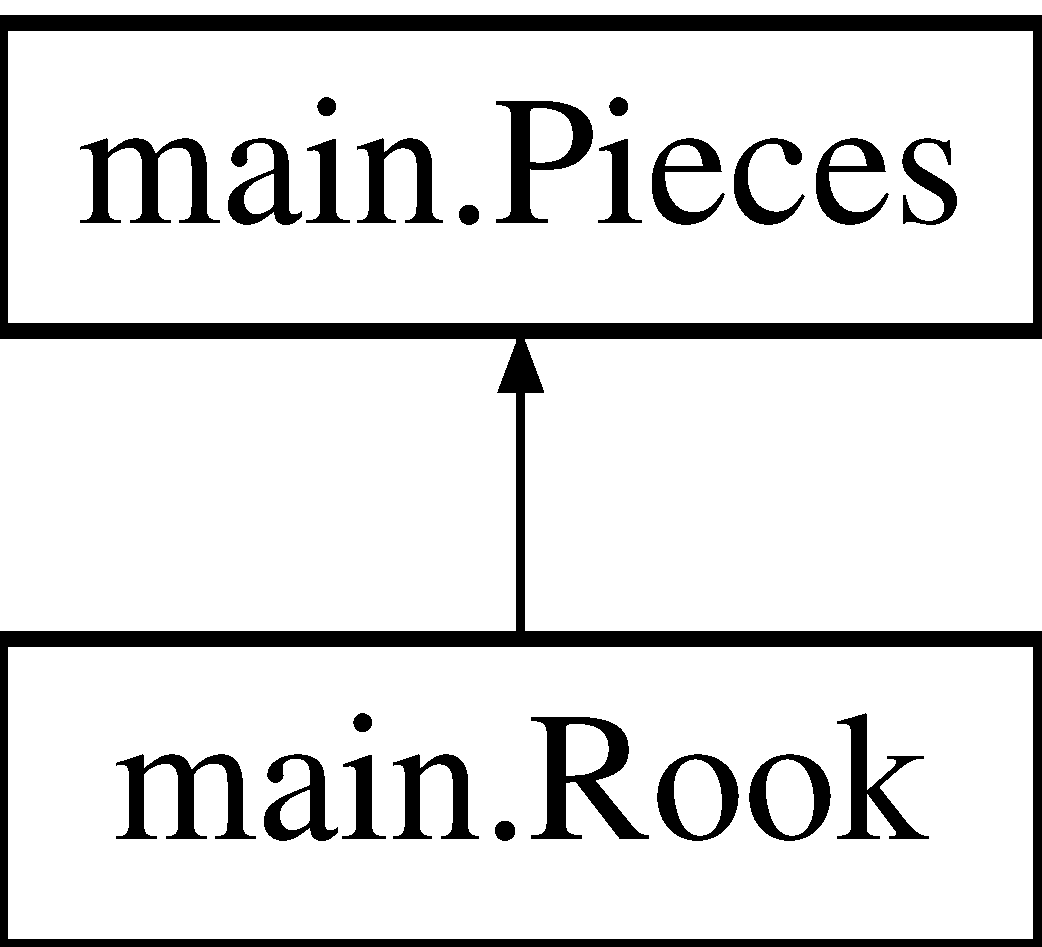
\includegraphics[height=2.000000cm]{classmain_1_1_rook}
\end{center}
\end{figure}
\subsection*{Public Member Functions}
\begin{DoxyCompactItemize}
\item 
\mbox{\hyperlink{classmain_1_1_rook_a6b0bbb8687463b828687c62b858cc479}{Rook}} (int x, int y, int player)
\item 
boolean \mbox{\hyperlink{classmain_1_1_rook_a83d5128f2957334e011560ae9d2f5f92}{is\+Valid\+Move}} (int newX, int newY)
\item 
boolean \mbox{\hyperlink{classmain_1_1_rook_a2b4fa722d895acc10aeae86c50d1a911}{valid\+Move}} (int newX, int newY, \mbox{\hyperlink{classmain_1_1_board}{Board}} board)
\item 
boolean \mbox{\hyperlink{classmain_1_1_rook_ad78bc0a0dc96db23b2476b897722371c}{could\+Be\+Stopped}} (int newX, int newY, \mbox{\hyperlink{classmain_1_1_board}{Board}} board)
\item 
boolean \mbox{\hyperlink{classmain_1_1_rook_ac94718e4402dc3f01761ec2503fb1c13}{is\+Movable}} (\mbox{\hyperlink{classmain_1_1_board}{Board}} board)
\end{DoxyCompactItemize}
\subsection*{Additional Inherited Members}


\subsection{Detailed Description}
\begin{DoxyAuthor}{Author}
kaichenle 
\end{DoxyAuthor}


\subsection{Constructor \& Destructor Documentation}
\mbox{\Hypertarget{classmain_1_1_rook_a6b0bbb8687463b828687c62b858cc479}\label{classmain_1_1_rook_a6b0bbb8687463b828687c62b858cc479}} 
\index{main\+::\+Rook@{main\+::\+Rook}!Rook@{Rook}}
\index{Rook@{Rook}!main\+::\+Rook@{main\+::\+Rook}}
\subsubsection{\texorpdfstring{Rook()}{Rook()}}
{\footnotesize\ttfamily main.\+Rook.\+Rook (\begin{DoxyParamCaption}\item[{int}]{x,  }\item[{int}]{y,  }\item[{int}]{player }\end{DoxyParamCaption})\hspace{0.3cm}{\ttfamily [inline]}}

constructor 
\begin{DoxyParams}{Parameters}
{\em x} & x\+Coord \\
\hline
{\em y} & y\+Coord \\
\hline
{\em player} & player 1 or 2 \\
\hline
\end{DoxyParams}


\subsection{Member Function Documentation}
\mbox{\Hypertarget{classmain_1_1_rook_ad78bc0a0dc96db23b2476b897722371c}\label{classmain_1_1_rook_ad78bc0a0dc96db23b2476b897722371c}} 
\index{main\+::\+Rook@{main\+::\+Rook}!could\+Be\+Stopped@{could\+Be\+Stopped}}
\index{could\+Be\+Stopped@{could\+Be\+Stopped}!main\+::\+Rook@{main\+::\+Rook}}
\subsubsection{\texorpdfstring{could\+Be\+Stopped()}{couldBeStopped()}}
{\footnotesize\ttfamily boolean main.\+Rook.\+could\+Be\+Stopped (\begin{DoxyParamCaption}\item[{int}]{newX,  }\item[{int}]{newY,  }\item[{\mbox{\hyperlink{classmain_1_1_board}{Board}}}]{board }\end{DoxyParamCaption})\hspace{0.3cm}{\ttfamily [inline]}}

if any pieces could stop input rook or queen(horizontal or vertical) piece from x,y to newX newY 
\begin{DoxyParams}{Parameters}
{\em newX} & end x\+Coord \\
\hline
{\em newY} & end y\+Coord \\
\hline
{\em board} & that the chess play on \\
\hline
\end{DoxyParams}
\begin{DoxyReturn}{Returns}
true if there is a piece exists that can stop the chess otherwise false 
\end{DoxyReturn}
\mbox{\Hypertarget{classmain_1_1_rook_ac94718e4402dc3f01761ec2503fb1c13}\label{classmain_1_1_rook_ac94718e4402dc3f01761ec2503fb1c13}} 
\index{main\+::\+Rook@{main\+::\+Rook}!is\+Movable@{is\+Movable}}
\index{is\+Movable@{is\+Movable}!main\+::\+Rook@{main\+::\+Rook}}
\subsubsection{\texorpdfstring{is\+Movable()}{isMovable()}}
{\footnotesize\ttfamily boolean main.\+Rook.\+is\+Movable (\begin{DoxyParamCaption}\item[{\mbox{\hyperlink{classmain_1_1_board}{Board}}}]{board }\end{DoxyParamCaption})\hspace{0.3cm}{\ttfamily [inline]}}

helper functions check movability of rook or queen(horizontal or vertical) 
\begin{DoxyParams}{Parameters}
{\em board} & the game will be on \\
\hline
\end{DoxyParams}
\begin{DoxyReturn}{Returns}
true if the input can move otherwise false 
\end{DoxyReturn}
\mbox{\Hypertarget{classmain_1_1_rook_a83d5128f2957334e011560ae9d2f5f92}\label{classmain_1_1_rook_a83d5128f2957334e011560ae9d2f5f92}} 
\index{main\+::\+Rook@{main\+::\+Rook}!is\+Valid\+Move@{is\+Valid\+Move}}
\index{is\+Valid\+Move@{is\+Valid\+Move}!main\+::\+Rook@{main\+::\+Rook}}
\subsubsection{\texorpdfstring{is\+Valid\+Move()}{isValidMove()}}
{\footnotesize\ttfamily boolean main.\+Rook.\+is\+Valid\+Move (\begin{DoxyParamCaption}\item[{int}]{newX,  }\item[{int}]{newY }\end{DoxyParamCaption})\hspace{0.3cm}{\ttfamily [inline]}}

see if the chess move against convention without consider other chesses \mbox{\Hypertarget{classmain_1_1_rook_a2b4fa722d895acc10aeae86c50d1a911}\label{classmain_1_1_rook_a2b4fa722d895acc10aeae86c50d1a911}} 
\index{main\+::\+Rook@{main\+::\+Rook}!valid\+Move@{valid\+Move}}
\index{valid\+Move@{valid\+Move}!main\+::\+Rook@{main\+::\+Rook}}
\subsubsection{\texorpdfstring{valid\+Move()}{validMove()}}
{\footnotesize\ttfamily boolean main.\+Rook.\+valid\+Move (\begin{DoxyParamCaption}\item[{int}]{newX,  }\item[{int}]{newY,  }\item[{\mbox{\hyperlink{classmain_1_1_board}{Board}}}]{board }\end{DoxyParamCaption})\hspace{0.3cm}{\ttfamily [inline]}}

Helper functions check if it is a valid path to move \mbox{\hyperlink{classmain_1_1_rook}{Rook}}. It will be called inside move\+Chess with is\+Valid\+Move in each pieces subclass. This will check if there are pieces on the board that will influence the fact if it is valid to move chess 
\begin{DoxyParams}{Parameters}
{\em newX} & end y\+Coord \\
\hline
{\em newY} & end y\+Coord \\
\hline
{\em board} & the chess play on \\
\hline
\end{DoxyParams}
\begin{DoxyReturn}{Returns}
true if valid otherwise false 
\end{DoxyReturn}


The documentation for this class was generated from the following file\+:\begin{DoxyCompactItemize}
\item 
main/Rook.\+java\end{DoxyCompactItemize}

\hypertarget{classtests_1_1_rook_tests}{}\section{tests.\+Rook\+Tests Class Reference}
\label{classtests_1_1_rook_tests}\index{tests.\+Rook\+Tests@{tests.\+Rook\+Tests}}
\subsection*{Public Member Functions}
\begin{DoxyCompactItemize}
\item 
void \mbox{\hyperlink{classtests_1_1_rook_tests_a0c22f41e6a959108015b6d6a17adebef}{should\+Move\+Rook}} ()
\end{DoxyCompactItemize}


\subsection{Detailed Description}
\begin{DoxyAuthor}{Author}
kaichenle 
\end{DoxyAuthor}


\subsection{Member Function Documentation}
\mbox{\Hypertarget{classtests_1_1_rook_tests_a0c22f41e6a959108015b6d6a17adebef}\label{classtests_1_1_rook_tests_a0c22f41e6a959108015b6d6a17adebef}} 
\index{tests\+::\+Rook\+Tests@{tests\+::\+Rook\+Tests}!should\+Move\+Rook@{should\+Move\+Rook}}
\index{should\+Move\+Rook@{should\+Move\+Rook}!tests\+::\+Rook\+Tests@{tests\+::\+Rook\+Tests}}
\subsubsection{\texorpdfstring{should\+Move\+Rook()}{shouldMoveRook()}}
{\footnotesize\ttfamily void tests.\+Rook\+Tests.\+should\+Move\+Rook (\begin{DoxyParamCaption}{ }\end{DoxyParamCaption})\hspace{0.3cm}{\ttfamily [inline]}}

test on move\+Chess 

The documentation for this class was generated from the following file\+:\begin{DoxyCompactItemize}
\item 
tests/Rook\+Tests.\+java\end{DoxyCompactItemize}

\hypertarget{classtests_1_1_stalemate_tests}{}\section{tests.\+Stalemate\+Tests Class Reference}
\label{classtests_1_1_stalemate_tests}\index{tests.\+Stalemate\+Tests@{tests.\+Stalemate\+Tests}}
\subsection*{Public Member Functions}
\begin{DoxyCompactItemize}
\item 
void \mbox{\hyperlink{classtests_1_1_stalemate_tests_a20c3f727a381198c62311aab0e76f53d}{movable\+Bishop\+Or\+Queen\+Tests}} ()
\item 
void \mbox{\hyperlink{classtests_1_1_stalemate_tests_a986921c05431c7eaaed69a8b2f63aee1}{movable\+Rook\+Or\+Queen\+Tests}} ()
\item 
void \mbox{\hyperlink{classtests_1_1_stalemate_tests_a1c33d7510b52a84bdbe26b101b52972d}{movable\+Kinght\+Tests}} ()
\item 
void \mbox{\hyperlink{classtests_1_1_stalemate_tests_a0202b8146eec4cec68329eec56dc71e4}{movable\+Pawn\+Tests}} ()
\item 
void \mbox{\hyperlink{classtests_1_1_stalemate_tests_a81624d7ceeff6b67b2c35d0cef08f467}{basic\+Stalemate\+Test}} ()
\item 
void \mbox{\hyperlink{classtests_1_1_stalemate_tests_a4873edea4e4df4a2d093a0da968c2ce9}{wiki\+Stalemate\+Test}} ()
\end{DoxyCompactItemize}


\subsection{Detailed Description}
\begin{DoxyAuthor}{Author}
kaichenle 
\end{DoxyAuthor}


\subsection{Member Function Documentation}
\mbox{\Hypertarget{classtests_1_1_stalemate_tests_a81624d7ceeff6b67b2c35d0cef08f467}\label{classtests_1_1_stalemate_tests_a81624d7ceeff6b67b2c35d0cef08f467}} 
\index{tests\+::\+Stalemate\+Tests@{tests\+::\+Stalemate\+Tests}!basic\+Stalemate\+Test@{basic\+Stalemate\+Test}}
\index{basic\+Stalemate\+Test@{basic\+Stalemate\+Test}!tests\+::\+Stalemate\+Tests@{tests\+::\+Stalemate\+Tests}}
\subsubsection{\texorpdfstring{basic\+Stalemate\+Test()}{basicStalemateTest()}}
{\footnotesize\ttfamily void tests.\+Stalemate\+Tests.\+basic\+Stalemate\+Test (\begin{DoxyParamCaption}{ }\end{DoxyParamCaption})\hspace{0.3cm}{\ttfamily [inline]}}

basic test on is\+Stalemate \mbox{\Hypertarget{classtests_1_1_stalemate_tests_a20c3f727a381198c62311aab0e76f53d}\label{classtests_1_1_stalemate_tests_a20c3f727a381198c62311aab0e76f53d}} 
\index{tests\+::\+Stalemate\+Tests@{tests\+::\+Stalemate\+Tests}!movable\+Bishop\+Or\+Queen\+Tests@{movable\+Bishop\+Or\+Queen\+Tests}}
\index{movable\+Bishop\+Or\+Queen\+Tests@{movable\+Bishop\+Or\+Queen\+Tests}!tests\+::\+Stalemate\+Tests@{tests\+::\+Stalemate\+Tests}}
\subsubsection{\texorpdfstring{movable\+Bishop\+Or\+Queen\+Tests()}{movableBishopOrQueenTests()}}
{\footnotesize\ttfamily void tests.\+Stalemate\+Tests.\+movable\+Bishop\+Or\+Queen\+Tests (\begin{DoxyParamCaption}{ }\end{DoxyParamCaption})\hspace{0.3cm}{\ttfamily [inline]}}

test on movable\+Bishop\+Or\+Queen \mbox{\Hypertarget{classtests_1_1_stalemate_tests_a1c33d7510b52a84bdbe26b101b52972d}\label{classtests_1_1_stalemate_tests_a1c33d7510b52a84bdbe26b101b52972d}} 
\index{tests\+::\+Stalemate\+Tests@{tests\+::\+Stalemate\+Tests}!movable\+Kinght\+Tests@{movable\+Kinght\+Tests}}
\index{movable\+Kinght\+Tests@{movable\+Kinght\+Tests}!tests\+::\+Stalemate\+Tests@{tests\+::\+Stalemate\+Tests}}
\subsubsection{\texorpdfstring{movable\+Kinght\+Tests()}{movableKinghtTests()}}
{\footnotesize\ttfamily void tests.\+Stalemate\+Tests.\+movable\+Kinght\+Tests (\begin{DoxyParamCaption}{ }\end{DoxyParamCaption})\hspace{0.3cm}{\ttfamily [inline]}}

test on movable\+Knight \mbox{\Hypertarget{classtests_1_1_stalemate_tests_a0202b8146eec4cec68329eec56dc71e4}\label{classtests_1_1_stalemate_tests_a0202b8146eec4cec68329eec56dc71e4}} 
\index{tests\+::\+Stalemate\+Tests@{tests\+::\+Stalemate\+Tests}!movable\+Pawn\+Tests@{movable\+Pawn\+Tests}}
\index{movable\+Pawn\+Tests@{movable\+Pawn\+Tests}!tests\+::\+Stalemate\+Tests@{tests\+::\+Stalemate\+Tests}}
\subsubsection{\texorpdfstring{movable\+Pawn\+Tests()}{movablePawnTests()}}
{\footnotesize\ttfamily void tests.\+Stalemate\+Tests.\+movable\+Pawn\+Tests (\begin{DoxyParamCaption}{ }\end{DoxyParamCaption})\hspace{0.3cm}{\ttfamily [inline]}}

test on movable\+Pawn \mbox{\Hypertarget{classtests_1_1_stalemate_tests_a986921c05431c7eaaed69a8b2f63aee1}\label{classtests_1_1_stalemate_tests_a986921c05431c7eaaed69a8b2f63aee1}} 
\index{tests\+::\+Stalemate\+Tests@{tests\+::\+Stalemate\+Tests}!movable\+Rook\+Or\+Queen\+Tests@{movable\+Rook\+Or\+Queen\+Tests}}
\index{movable\+Rook\+Or\+Queen\+Tests@{movable\+Rook\+Or\+Queen\+Tests}!tests\+::\+Stalemate\+Tests@{tests\+::\+Stalemate\+Tests}}
\subsubsection{\texorpdfstring{movable\+Rook\+Or\+Queen\+Tests()}{movableRookOrQueenTests()}}
{\footnotesize\ttfamily void tests.\+Stalemate\+Tests.\+movable\+Rook\+Or\+Queen\+Tests (\begin{DoxyParamCaption}{ }\end{DoxyParamCaption})\hspace{0.3cm}{\ttfamily [inline]}}

test on movable\+Rook\+Or\+Queen \mbox{\Hypertarget{classtests_1_1_stalemate_tests_a4873edea4e4df4a2d093a0da968c2ce9}\label{classtests_1_1_stalemate_tests_a4873edea4e4df4a2d093a0da968c2ce9}} 
\index{tests\+::\+Stalemate\+Tests@{tests\+::\+Stalemate\+Tests}!wiki\+Stalemate\+Test@{wiki\+Stalemate\+Test}}
\index{wiki\+Stalemate\+Test@{wiki\+Stalemate\+Test}!tests\+::\+Stalemate\+Tests@{tests\+::\+Stalemate\+Tests}}
\subsubsection{\texorpdfstring{wiki\+Stalemate\+Test()}{wikiStalemateTest()}}
{\footnotesize\ttfamily void tests.\+Stalemate\+Tests.\+wiki\+Stalemate\+Test (\begin{DoxyParamCaption}{ }\end{DoxyParamCaption})\hspace{0.3cm}{\ttfamily [inline]}}

test on example from wiki 

The documentation for this class was generated from the following file\+:\begin{DoxyCompactItemize}
\item 
tests/Stalemate\+Tests.\+java\end{DoxyCompactItemize}

\hypertarget{class_g_u_i_1_1_g_u_i_board_1_1_table}{}\section{G\+U\+I.\+G\+U\+I\+Board.\+Table Class Reference}
\label{class_g_u_i_1_1_g_u_i_board_1_1_table}\index{G\+U\+I.\+G\+U\+I\+Board.\+Table@{G\+U\+I.\+G\+U\+I\+Board.\+Table}}
Inheritance diagram for G\+U\+I.\+G\+U\+I\+Board.\+Table\+:\begin{figure}[H]
\begin{center}
\leavevmode
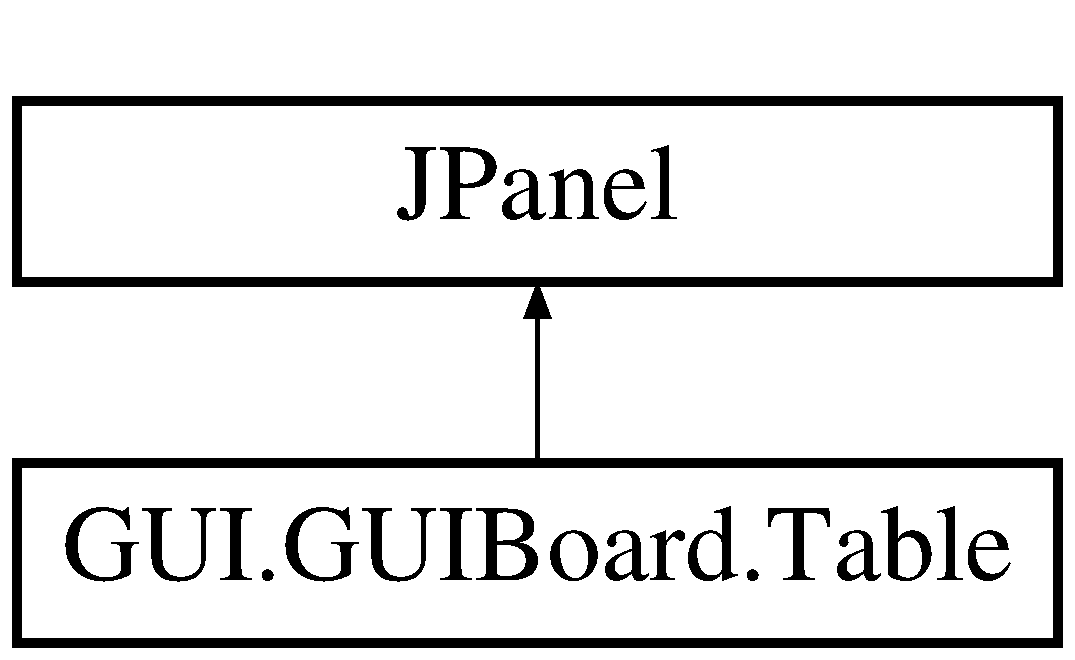
\includegraphics[height=2.000000cm]{class_g_u_i_1_1_g_u_i_board_1_1_table}
\end{center}
\end{figure}
\subsection*{Public Member Functions}
\begin{DoxyCompactItemize}
\item 
\mbox{\Hypertarget{class_g_u_i_1_1_g_u_i_board_1_1_table_a82aa9ac4273939eee2c6ca71c814c622}\label{class_g_u_i_1_1_g_u_i_board_1_1_table_a82aa9ac4273939eee2c6ca71c814c622}} 
{\bfseries Table} (\mbox{\hyperlink{class_g_u_i_1_1_main}{Main}} main)
\item 
void \mbox{\hyperlink{class_g_u_i_1_1_g_u_i_board_1_1_table_a311b401d6ee3d8e7a391a6b20e476de4}{move\+Icon}} (int player, J\+Button end\+Button)
\item 
void \mbox{\hyperlink{class_g_u_i_1_1_g_u_i_board_1_1_table_a4cfeeb28e2ada796495560fc712ed32f}{change\+Button\+Color\+Back}} (J\+Button button)
\item 
void \mbox{\hyperlink{class_g_u_i_1_1_g_u_i_board_1_1_table_abb7c7199330206d15dc1b072f93ecf6e}{undo}} ()
\end{DoxyCompactItemize}
\subsection*{Public Attributes}
\begin{DoxyCompactItemize}
\item 
\mbox{\Hypertarget{class_g_u_i_1_1_g_u_i_board_1_1_table_ab201418f9a4e484b19f11d0d8880c49a}\label{class_g_u_i_1_1_g_u_i_board_1_1_table_ab201418f9a4e484b19f11d0d8880c49a}} 
J\+Button {\bfseries chess\+Panel} \mbox{[}$\,$\mbox{]}\mbox{[}$\,$\mbox{]}
\item 
\mbox{\Hypertarget{class_g_u_i_1_1_g_u_i_board_1_1_table_a13dfe45b9428e15f35a1f0bd5054ace4}\label{class_g_u_i_1_1_g_u_i_board_1_1_table_a13dfe45b9428e15f35a1f0bd5054ace4}} 
Dimension {\bfseries O\+U\+T\+\_\+\+F\+R\+A\+M\+E\+\_\+\+D\+I\+M\+E\+N\+S\+I\+ON} = new Dimension(600, 600)
\end{DoxyCompactItemize}


\subsection{Member Function Documentation}
\mbox{\Hypertarget{class_g_u_i_1_1_g_u_i_board_1_1_table_a4cfeeb28e2ada796495560fc712ed32f}\label{class_g_u_i_1_1_g_u_i_board_1_1_table_a4cfeeb28e2ada796495560fc712ed32f}} 
\index{G\+U\+I\+::\+G\+U\+I\+Board\+::\+Table@{G\+U\+I\+::\+G\+U\+I\+Board\+::\+Table}!change\+Button\+Color\+Back@{change\+Button\+Color\+Back}}
\index{change\+Button\+Color\+Back@{change\+Button\+Color\+Back}!G\+U\+I\+::\+G\+U\+I\+Board\+::\+Table@{G\+U\+I\+::\+G\+U\+I\+Board\+::\+Table}}
\subsubsection{\texorpdfstring{change\+Button\+Color\+Back()}{changeButtonColorBack()}}
{\footnotesize\ttfamily void G\+U\+I.\+G\+U\+I\+Board.\+Table.\+change\+Button\+Color\+Back (\begin{DoxyParamCaption}\item[{J\+Button}]{button }\end{DoxyParamCaption})\hspace{0.3cm}{\ttfamily [inline]}}

change the selected button back to original color 
\begin{DoxyParams}{Parameters}
{\em button} & the button that need to set the color back \\
\hline
\end{DoxyParams}
\mbox{\Hypertarget{class_g_u_i_1_1_g_u_i_board_1_1_table_a311b401d6ee3d8e7a391a6b20e476de4}\label{class_g_u_i_1_1_g_u_i_board_1_1_table_a311b401d6ee3d8e7a391a6b20e476de4}} 
\index{G\+U\+I\+::\+G\+U\+I\+Board\+::\+Table@{G\+U\+I\+::\+G\+U\+I\+Board\+::\+Table}!move\+Icon@{move\+Icon}}
\index{move\+Icon@{move\+Icon}!G\+U\+I\+::\+G\+U\+I\+Board\+::\+Table@{G\+U\+I\+::\+G\+U\+I\+Board\+::\+Table}}
\subsubsection{\texorpdfstring{move\+Icon()}{moveIcon()}}
{\footnotesize\ttfamily void G\+U\+I.\+G\+U\+I\+Board.\+Table.\+move\+Icon (\begin{DoxyParamCaption}\item[{int}]{player,  }\item[{J\+Button}]{end\+Button }\end{DoxyParamCaption})\hspace{0.3cm}{\ttfamily [inline]}}

change the icon if it was a valid move 
\begin{DoxyParams}{Parameters}
{\em player} & player to check checkmate on \\
\hline
{\em end\+Button} & the grid need to update icon \\
\hline
\end{DoxyParams}
\mbox{\Hypertarget{class_g_u_i_1_1_g_u_i_board_1_1_table_abb7c7199330206d15dc1b072f93ecf6e}\label{class_g_u_i_1_1_g_u_i_board_1_1_table_abb7c7199330206d15dc1b072f93ecf6e}} 
\index{G\+U\+I\+::\+G\+U\+I\+Board\+::\+Table@{G\+U\+I\+::\+G\+U\+I\+Board\+::\+Table}!undo@{undo}}
\index{undo@{undo}!G\+U\+I\+::\+G\+U\+I\+Board\+::\+Table@{G\+U\+I\+::\+G\+U\+I\+Board\+::\+Table}}
\subsubsection{\texorpdfstring{undo()}{undo()}}
{\footnotesize\ttfamily void G\+U\+I.\+G\+U\+I\+Board.\+Table.\+undo (\begin{DoxyParamCaption}{ }\end{DoxyParamCaption})\hspace{0.3cm}{\ttfamily [inline]}}

change icon when undo is requested 

The documentation for this class was generated from the following file\+:\begin{DoxyCompactItemize}
\item 
G\+U\+I/G\+U\+I\+Board.\+java\end{DoxyCompactItemize}

\hypertarget{classtests_1_1_undo_tests}{}\section{tests.\+Undo\+Tests Class Reference}
\label{classtests_1_1_undo_tests}\index{tests.\+Undo\+Tests@{tests.\+Undo\+Tests}}
\subsection*{Public Member Functions}
\begin{DoxyCompactItemize}
\item 
\mbox{\Hypertarget{classtests_1_1_undo_tests_a63bfab73d9714ce1e1928cd2008fe9be}\label{classtests_1_1_undo_tests_a63bfab73d9714ce1e1928cd2008fe9be}} 
void {\bfseries undo\+Test} ()
\item 
\mbox{\Hypertarget{classtests_1_1_undo_tests_ae95dec01298d257be5ddd0f5e83b4d99}\label{classtests_1_1_undo_tests_ae95dec01298d257be5ddd0f5e83b4d99}} 
void {\bfseries get\+Turns\+Test} ()
\end{DoxyCompactItemize}


\subsection{Detailed Description}
\begin{DoxyAuthor}{Author}
kaichenle 
\end{DoxyAuthor}


The documentation for this class was generated from the following file\+:\begin{DoxyCompactItemize}
\item 
tests/Undo\+Tests.\+java\end{DoxyCompactItemize}

%--- End generated contents ---

% Index
\backmatter
\newpage
\phantomsection
\clearemptydoublepage
\addcontentsline{toc}{chapter}{Index}
\printindex

\end{document}
